\documentclass[a4paper,10pt]{book}
\usepackage[a4paper, total={6in, 8in}]{geometry}
\usepackage[utf8]{inputenc}
\usepackage{tikz}
\usetikzlibrary{arrows.meta}
\usepackage{mathrsfs}
\usepackage{amsmath,amsfonts,amssymb,bm}
\usepackage{hyperref}
\usepackage{pgfplots}
\usetikzlibrary{math} %needed tikz library
\usepackage{bm}
\usepackage{appendix}
\usepackage{algorithm}
%\usepackage{arevmath}     % For math symbols
\usepackage[noend]{algpseudocode}


\newcommand{\example}[1]{\vspace{0.2cm}\framebox[0.92\textwidth]{ \parbox[c]{0.9\textwidth}{{\bf Example: }  #1}}\vspace{0.2cm}}

\def\ud{\mathrm{d}}
\def\E{\mathrm{E}}
\def\pij{p_{ij}}
\def\part{\partial}
\def\<{\langle}
\def\>{\rangle}
\def\ux{\underline{x}}
%\newcommand{\bm}[1]{\boldmath{ #1}}
%opening


 {%
   \definecolor{BLACK}{gray}{0}
   \definecolor{WHITE}{gray}{1}
   \definecolor{RED}{rgb}{1,0,0}
   \definecolor{GREEN}{rgb}{0,1,0}
   \definecolor{BLUE}{rgb}{0,0,1}
   \definecolor{CYAN}{cmyk}{1,0,0,0}
   \definecolor{MAGENTA}{cmyk}{0,1,0,0}
   \definecolor{YELLOW}{cmyk}{0,0,1,0}
 }

%%%%%%%%%%%%%%%%%%%%%%%%%%%%%% User specified LaTeX commands.

%\usepackage{epsfig,amssymb, color}

\DeclareMathOperator*{\argmax}{arg\,max}
\DeclareMathOperator*{\argmin}{arg\,min}
\newcommand{\1}{\mathbb I}
\newcommand{\p}{\mathbbm P}
\newcommand{\sign}{\mathrm{sign}}
\newcommand{\bx}{\mathbf x}
\newcommand{\bt}{\mathbf t}
\newcommand{\dd}{\partial}
\newcommand{\sm}{\setminus}


\title{Lecture notes: Epidemics on Networks}
\author{Dr. Alejandro Lage Castellanos, and ChatGPT4}

\makeindex

\begin{document}
\maketitle
\tableofcontents
% 
% \begin{abstract}
% 
% \end{abstract}

%\index
 \chapter{Classical results in mathematical epidemiology}


Epidemics are typical examples of complex phenomena. A mathematical description of an epidemic needs to take into account its non deterministic nature, and, therefore, rely on probabilities. An epidemic process is, essentially, a stochastic process. 

In the dawn of mathematical epidemiology, researchers studied the dynamics in time of probabilities regarding the states of individuals. This is the case of  the study of life expectancy and smallpox by Daniel Bernoulli, and so is the famous contribution of Kermac y McEndrick with the SIR models. In both cases, the resulting dynamic equations correspond to the Master equation of the given stochastic processes.


\section{A supersonic intro to Master equation}

%\section{Stochastic processes and Master equation}

\subsection*{Introduction to Stochastic Processes and Markov Chains}

A \textbf{stochastic process} is a mathematical model that describes the evolution of a random system over time. It's a collection of random variables indexed by time, and can be used to model a wide range of phenomena, from the stock market to the weather.

A \textbf{Markov chain} is a specific type of stochastic process that has the \textbf{Markov property}: the future state of the system only depends on the current state, and not on any of the previous states. This makes Markov chains particularly useful for modeling systems where the future is dependent on the present, but not on the past.

Formally, a Markov chain is a sequence of random variables $X_0, X_1, X_2, \ldots$ that take values in a finite or countable set $S$, where the probability of moving from one state to another depends only on the current state. That is, for all $n \geq 0$ and all states $i, j \in S$,

\begin{equation*}
    \mathbb{P}(X_{t+1} = j \mid X_t = i, X_{t-1} = i_{t-1}, \ldots, X_0 = i_0) = \mathbb{P}(X_{t+1} = j \mid X_t = i).
\end{equation*}

Markov chains have many interesting properties and applications, including their use in modeling queueing systems, random walks, and machine learning algorithms.


\subsection*{Master equation}

The Master Equation is a fundamental tool in the study of stochastic processes, particularly in probability theory and statistical physics. It describes the time evolution of the probability distribution of a system in terms of transition rates between different states. In its simplest form, the Master Equation takes the form of a first-order differential equation:

\begin{equation}
    \frac{d}{dt} P_i(t) = \sum_j W_{ji} P_j(t) - \sum_j W_{ij} P_i(t),
\end{equation}
where $P_i(t)$ is the probability of the system being in state $i$ at time $t$, and $W_{ij}$ is the transition rate from state $j$ to state $i$. The first term on the right-hand side of the equation represents the rate of transitions from all other states $j$ to state $i$, weighted by the probability of being in state $j$. The second term represents the rate of transitions from state $i$ to all other states $j$, weighted by the probability of being in state $i$.

Master equation can be seen as a continuity equation, or a mass conservation equation. In fluid dynamics, for instance, the rate of change of mass in a control volume must be equal to the net rate of mass flow into or out of the control volume. Mathematically, the continuity equation can be written as:
$$\frac{\partial \rho}{\partial t} + \nabla \cdot (\rho \mathbf{v}) = \qquad \frac{d}{dt} \int_V   \rho \: \ud V +  \oint_S  \rho \mathbf{v} \cdot \ud \mathbf{S} = 0$$
where $\rho$ is the fluid density, $\mathbf{v}$ is the velocity vector, $\frac{\partial \rho}{\partial t}$ is the rate of change of density with respect to time, and $\nabla \cdot (\rho \mathbf{v})$ is the divergence of the mass flux density vector.

In other words, the continuity equation states that the change in the amount of fluid within a control volume is equal to the net flow of fluid across the boundaries of that control volume. This principle is based on the law of conservation of mass, which states that mass cannot be created or destroyed, only transferred or transformed.

\subsubsection*{\bf Drunken man}

A drunken man is moving around his own house, which is made of a Bedroom, a Bathroom, a Livingroom and a Kitchen, connected through doors as shown in the diagram:
\[
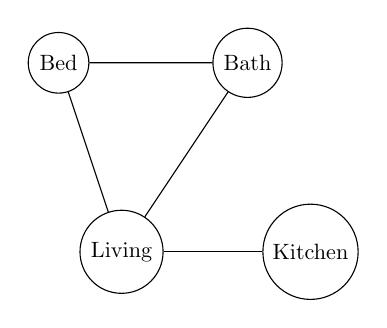
\begin{tikzpicture}[scale=0.8, transform shape]
    \node[shape=circle,draw=black] (1) at (0,3) {Bed};
    \node[shape=circle,draw=black] (2) at (3,3) {Bath};
    \node[shape=circle,draw=black] (3) at (1,0) {Living};
    \node[shape=circle,draw=black] (4) at (4,0) {Kitchen};
    \draw[-] (1) -- (2);
    \draw[-] (1) -- (3);
    \draw[-] (2) -- (3);
    \draw[-] (3) -- (4);
\end{tikzpicture} 
\]
Everytime he enters a room, he chooses one of the doors in that room at random, and moves throuhg it to the next room. The man starts in his bedroom.

\begin{enumerate}
 \item What is the shortest path from the bedroom to the kitchen?
 \item What is the largest path between bed and kitchen (without cycles)?
 \item If the man keeps walking for a very long time, what amount of time he spends in every room?las
 \item What is the expected time that takes the man to visit the kitchen for the first time?
\end{enumerate}

{\bf Solution in discrete time:}

Let $\vec p(t) = (p_1,p_2,p_3,p_3)$ be the vector state defining the probabilities, at time $t$ of finding the drunken man at (bed,bath,living,kitchen), respectively. This can be seen as the following set of stochastic decaying chemical reactions:
\begin{eqnarray*}
 \mbox{Bed}  &\mathrel{\mathop{\rightleftharpoons}\limits^{\delta/2}_{\delta/2}}& \mbox{Bath} \\
  \mbox{Bed}  &\mathrel{\mathop{\rightleftharpoons}\limits^{\delta/2}_{\delta/3}}& \mbox{Living} \\
  \mbox{Bath}  &\mathrel{\mathop{\rightleftharpoons}\limits^{\delta/2}_{\delta/3}}& \mbox{Living} \\
  \mbox{Living}  &\mathrel{\mathop{\rightleftharpoons}\limits^{\delta/3}_{\delta}}& \mbox{Kitchen} 
\end{eqnarray*}


Consider the transition matrix
\[
M = \begin{bmatrix}
1-\delta & \delta/2 & \delta/3 & 0\\
\delta/2 & 1-\delta & \delta/3 & 0\\
\delta/2 & \delta/2 & 1-\delta & \delta\\
0 & 0 & \delta/3 & 1-\delta
\end{bmatrix}\]
such that the evolution in discrete time of the Markov process is given by
\[ \vec p(k+1) = M \cdot \vec p(k) \]
So the full evolution from $t=0$ to $t$ is given by
\[ \vec p (k) = M^k \vec p(0)\]

Matrices as $M$, postive in their values, and such that every column add to 1, are known as stochastic matrices. It can be shown that the largest eigevanlue, in any stochastic matrix, is $\lambda = 1$, and its  eigenvector is a probability vector.

In the current case, it is easy to prove, by substitution, that $\vec p_\infty = (2,2,3,1)/8$ is such eigenvecto. This implies that
\[ \vec p_\infty = M\cdot \vec p_\infty\]
meaning that $\vec p_\infty$ is the stationary solution of the process.

A simple generalization proves that an umbiased random walk on a graph has a steaty state probability that only depends on the degree of each node, and its proportional to it.

{\bf Take home message:} every discrete time homogenous in time Markov process corresponds to a transition (stochastic) matrix, whose $\lambda=1$ eigenvector is the long time limit of the process.

{\bf Continuous time limit:}

We can consider the scaling of this process as we devide the time scale in T units, and send $\delta \to \delta / T$. This process is known as continuous time limit, when $T\to \infty$. In this case
\[  \vec p(k+1) - \vec p(k) = \left( M(\delta/T) - \mathbb{I}\right) \cdot \vec  p(k)\]
resulting in 
\[ \frac {\ud \vec p}{\ud t}  =  \left(M(\delta)-\mathbb I \right) \cdot \vec p\]
Which also shows that the stationary solution is given by 
\[ \frac {\ud \vec p}{\ud t}  = 0 \quad  \Rightarrow   \left(M(\delta)-\mathbb I \right) \cdot \vec p = 0\]
which is the defintion of the eigenvalue $\lambda = 1$ for matrix $M$.

Attention, this eigenvector might not be unique. If it is unique, it is the solution in the long time limit. If it is not unique, then the solution will depend on the initial conditions.


\section{Daniel Bernoulli and smallpox}

Daniel Bernoulli's study of the effect of smallpox in life expentancy and the possibility of innoculation as a vaccination strategy, a debated argument in the Royal Academy of Science in Paris, in the second half of the XVIII century.

Effect of innoculation in Smallpox, 
Royal Academy of Science, Paris, 1760, published in 1766

Scope: calculate the gain in life expectancy at birth if smallpox were to be eliminated as a cause of death. The model assumes a fixed amount of infections every year, so, it is not a model for the infection. Still, it deals with relevant questions in epidemiology.

The model of Bernoulli studied the age dynamics of the entire population in a country, as classified in three groups: susceptibles, immunes and dead\footnote{ As you can see, there is no characterization of those that are currently infected. The reason for this is that the study considered  large time scales, such that the actual infectious period was neglible in that scale, and people were considered to transition immediately between susceptible to immune.}. Susceptible was everyone that had not been in conctact with the disease. Immune was everyone that had passed the disease. Dead were those that died, either from the disease or from other causes. Smallpox could either cause death, or cause life-long immunity. So, it is considered one of the SIR family of models, but rather, in this case, SR model.

 


\[
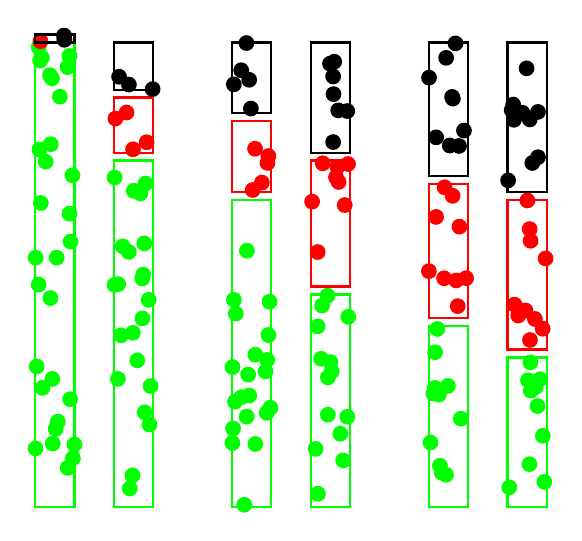
\begin{tikzpicture}
 \def\dx{0.5}
 \def\oldy{0}
 \def\x{0}
 \foreach \y / \col  [remember=\y as \oldy] in {6/green, 6/red, 6/black}
  {
    \draw[\col,thick] (\x,\oldy+0.1) rectangle (\x+\dx,\y);
    \tikzmath{\he = \y-\oldy-0.1;\points = int( 5*(\y-\oldy)); }
    \foreach \i in {1,...,\points}
    {       \fill[\col] (\x+\dx*random,\oldy+0.1 + \he *random) circle (0.1);
    }
  }
 \def\oldy{0}
 \def\x{1.0}
 \foreach \y / \col  [remember=\y as \oldy] in {4.5/green, 5.3/red, 6/black}
  {
    \draw[\col,thick] (\x,\oldy+0.1) rectangle (\x+\dx,\y);
    \tikzmath{\he = \y-\oldy-0.1;\points = int( 5*(\y-\oldy)); }
    \foreach \i in {1,...,\points}
    {       \fill[\col] (\x+\dx*random,\oldy+0.1 + \he *random) circle (0.1);
    }
  }

   \def\oldy{0}
 \def\x{2.5}
 \foreach \y / \col  [remember=\y as \oldy] in {4/green, 5/red, 6/black}
  {
    \draw[\col,thick] (\x,\oldy+0.1) rectangle (\x+\dx,\y);
    \tikzmath{\he = \y-\oldy-0.1; \points = int( 5*(\y-\oldy)); }
    \foreach \i in {1,...,\points}
    {       \fill[\col] (\x+\dx*random,\oldy+0.1 + \he *random) circle (0.1);
    }
  }
  
 \def\oldy{0}
 \def\x{3.5}
 \foreach \y / \col  [remember=\y as \oldy] in {2.8/green, 4.5/red, 6/black}
  {
    \draw[\col,thick] (\x,\oldy+0.1) rectangle (\x+\dx,\y);
    \tikzmath{\he = \y-\oldy-0.1; \points = int( 5*(\y-\oldy)); }
    \foreach \i in {1,...,\points}
    {       \fill[\col] (\x+\dx*random,\oldy+0.1 + \he *random) circle (0.1);
    }
  }  
  \def\oldy{0}
 \def\x{5}
 \foreach \y / \col  [remember=\y as \oldy] in {2.4/green, 4.2/red, 6/black}
  {
    \draw[\col,thick] (\x,\oldy+0.1) rectangle (\x+\dx,\y);
    \tikzmath{\he = \y-\oldy-0.1;\points = int( 5*(\y-\oldy)); }
    \foreach \i in {1,...,\points}
    {       \fill[\col] (\x+\dx*random,\oldy+0.1 + \he *random) circle (0.1);
    }
  }  
  \def\oldy{0}
 \def\x{6}
 \foreach \y / \col  [remember=\y as \oldy] in {2/green, 4/red, 6/black}
  {
    \draw[\col,thick] (\x,\oldy+0.1) rectangle (\x+\dx,\y);
    \tikzmath{\he = \y-\oldy-0.1;\points = int( 5*(\y-\oldy)); }
    \foreach \i in {1,...,\points}
    {       \fill[\col] (\x+\dx*random,\oldy+0.1 + \he *random) circle (0.1);
    }
  }  
% \def\r{7}
% \def\c{0}
% 
% \draw (\c,\c) circle (\r);
% 
% \foreach \x in {1,2,3,4,5,6}
% {
% \tikzmath{\r=\x/2;\c=\r/sqrt(2);}
% \draw (-\c, \c) circle (\r);
% \draw (\c, -\c) circle (\r); 
% }  
%   
%   \foreach \x / \col in {0/green, 1.2/red, 2.4/black, 3.6/blue, 4.8/orange}
%   {
%     \draw[\col,thick] (\x,0) rectangle (\x+0.8,2);
%     \foreach \i in {1,...,10}
%     {
%       \fill[\col] (\x+0.1*rand,0.1*rand+0.2*\i) circle (0.05);
%     }
%   }
%   \foreach \x in {0,1.2,2.4,3.6,4.8}
%   { 
%     \draw[green,thick] (\x,0) rectangle (\x+0.8,2);
%     \draw[red,thick] (\x,2.2) rectangle (\x+0.8,4.2);
%     \draw[black,thick] (\x,4.4) rectangle (\x+0.8,6.4);
%   }
\end{tikzpicture}
\]



Bernoulli imagined that people born in year $a=0$, could go through the states (un-infected, immune, dead) with certain probabilities \footnote{The transitions between this states were described as a Markov chain, although Markov contribution came centuries later.}
The dynamics relied on the following dynamic parameters:
\begin{itemize}
 \item $\mu(a)$ the rate of death of all causes except smallpox, for an individual of age $a$  
 \item $\beta$ is the {\bf force of infection}: the rate at which susceptible individual get infected
 \item $c = 1-s$ the fraction of individuals infected that dies of smallpox.
\end{itemize}

The Markov chain is described graphically as this:
\[
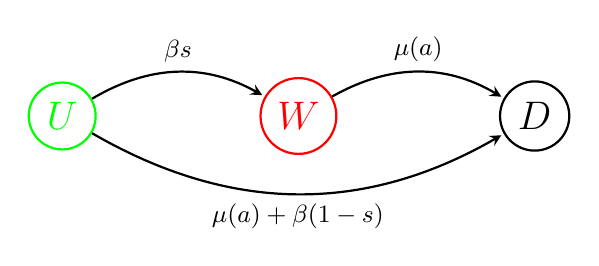
\begin{tikzpicture}[->,>=stealth,shorten >=1pt,auto,node distance=3cm, thick,main node/.style={circle,draw,font=\sffamily\Large\bfseries}]

  \node[main node, green] (U) {$U$};
  \node[main node, red] (W) [right of=U] {$W$};
  \node[main node] (D) [right of=W] {$D$};

  \path[every node/.style={font=\sffamily\small}]
    (U) edge [bend left] node [above] {$\beta s $} (W)
    (U) edge [bend right] node [below] {$\mu(a) + \beta (1-s) $} (D)
    (W) edge [bend left] node [above] {$\mu(a)$} (D);
\end{tikzpicture}
\]

The relevant quantities (dynamic variables) of the model depend on the age of the persons $a$. They are:
\begin{itemize}
 \item $u(a)$ the probability for an individual of being alive and susceptible (uninfected) at age $a$
 \item $w(a)$ the probability for an individual of being alive and immune at age $a$
 \item $d(a)$ is the probability of being dead at age $a$, but since probabilities add up to 1, and there are only three posible states, $d(a) = 1-u(a) -w(a)$.
 \end{itemize}

Considering the rates at which individuals can move from one state to the other, we can compute the contributions of each state in the Master equation. 
The dynamical system derived by Bernoulli is given by:
\begin{eqnarray*}
 \frac{\ud u}{\ud a} &=& -(\beta + \mu(a)) u(a) \\
 \frac{\ud w}{\ud a} &=& \beta (1-c) \mu(a) u(a) -\mu(a) w(a)
\end{eqnarray*}
The interest of Bernoulli was comparing the total amount of persons alive at a given age $u(a)+w(a)$ in the case where $c=0$ (people do not die of smallpox), and $c\neq 0$.

These equations  are recognized as one of the first modern mathematical approaches to mathematical epidemiology. Their solution and Bernoulli conclusions is out of the scope of the present course (if interested see \cite{dietz02}). However, its interpretation and derivation are useful to introduce some probabilistic methods and epidemic concepts. 

The Master Equation provides a powerful framework for analyzing a wide range of phenomena, including chemical reactions, population dynamics, and the behavior of complex systems. By solving the Master Equation, one can obtain the time-dependent probability distribution of the system, which can be used to calculate various statistical quantities of interest, such as the mean and variance of observables. The Master Equation can also be used to study the long-time behavior of the system, such as the emergence of steady-state solutions and the behavior of fluctuations around these solutions.

% Gossiping in science: Bernoulli in letter to Euler, discussing D’Alembert’s critics to his works: 
% \begin{quote}
% (...)je me trouve, trop souvent, injustement traitee dans ses ouvrages, j’ai pris la resolution depuis assez long-temps de ne rien lire qui sorte de sa plume (...) il semble que le succees de cette nouvelle analyse lui fit mal au coeur; il la critique de mille facons, toutes egalement ridicules et aprez l’avoir bien critiquee il se donne pour premier auteur d’une theeorie qu’il n’avoit pas seulement entendu nommer(...) Dolus an virtus quis in hoste requirat.
% \end{quote}
% The latin phrase, from Aeneid, translates to: What matters whether by valour or by stratagem we overcome the enemy?

\section{SIR compartmental models}
The SIR (Susceptible-Infectious-Recovered) model is a widely used mathematical framework for studying the spread of infectious diseases in populations. It  was first introduced by Kermack and McKendrick in a seminal paper published in 1927. They used a system of differential equations to describe the time evolution of the number of individuals in each compartment, and derived an expression for the critical threshold of the disease, above which an epidemic occurs. 
\[
\begin{tikzpicture}[
    declare function={a(\x)=0.75*\x-2;},
    declare function={b(\x)=\x;}
]
  \draw[thick] (0.5,0.4) rectangle (6.35,5.3); % draw the square
\begin{axis}[axis line style={opacity=0},
    domain=0:1,
%     axis lines=middle,
%     axis equal image,
     xtick=\empty, ytick=\empty
%     enlargelimits=true,
%     clip mode=individual, clip=false
]  
\addplot [red, only marks, mark=*, samples=50, mark size=2.5]    {rand};
\addplot [green, only marks, mark=*, samples=100, ma size=2.5]    {rand};
\addplot [black, only marks, mark=*, samples=50, mark size=2.5]    {rand};
%\addplot [thick] {a(x)};
%\addplot [thick] {b(x)};
  % draw labels
  \end{axis}
\end{tikzpicture} \]

A first idealization of what actually happens in an epidemic, is to think of society as a gas of individuals. Each individual can be in one of the following states:
\begin{itemize}
 \item {\bf Susceptible} individuals, who are at risk of becoming infected; 
 \item {\bf Infectious} individuals, who are capable of transmitting the disease to susceptible individuals;
 \item {\bf Recovered} individuals, who have either recovered from the disease and are immune, or have died from the disease, and are removed.
\end{itemize}

Under well mixed assumptions, this individuals-particles move around and interact with each other, occasionally. The process of contagion can be seen as a catalytic chemical reaction, in which the interaction of an Infectious individual with a Susceptible, can induce the latter to turn into infectious with a certain probability:
\begin{eqnarray*}
 S + I &\xrightarrow{\beta}& 2I \\
 I &\xrightarrow{\mu}& R \\
\end{eqnarray*}

Simulation of this process in a computer, relies on Monte Carlo methods, more precisely in action diffusion equations and Gillespie algorithm, that we will study later.
%Their work laid the foundation for the study of infectious disease dynamics, and has since been extended and modified in many ways to incorporate more complex disease transmission mechanisms and population structures.

A mean field probabilistic description can be made, by considering the population to be classified into three different compartments, according to their state:

\[
%     \begin{tikzpicture}
%         % Draw first urn
%         \draw (0,0) rectangle (1.5cm);
%                \foreach \i in {1,...,20}
%             \fill[black] (rand*1.5,rand*1.5) circle (0.1cm);
% 
%          \node at (0,-1.8) {Urn 1};
%         
%         % Draw second urn
%         \draw (5,0) circle (1.5cm);
%         \node at (5,-1.8) {Urn 2};
%         
% %         % Draw third urn
%         \draw (10,0) circle (1.5cm);
%         \node at (10,-1.8) {Urn 3};
   % \end{tikzpicture}
 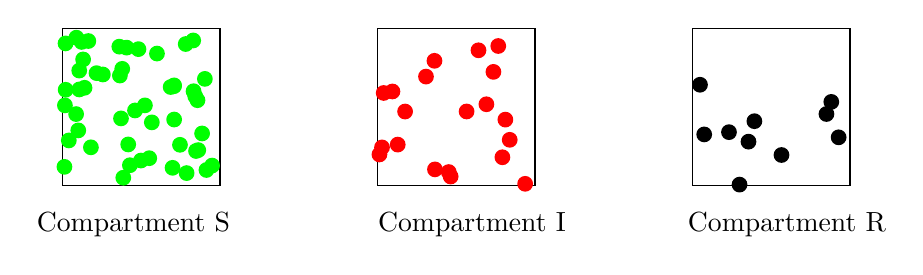
\begin{tikzpicture}
        % Draw first urn
        \draw (0,0) rectangle (2cm,2cm);
        \foreach \i in {1,...,50}
            \fill[green] (random*1.9,random*1.9) circle (0.1cm);
        \node at (0.9,-0.5) {Compartment S};
        
        % Draw second urn
        \draw (4,0) rectangle (6cm,2cm);
        \foreach \i in {1,...,20}
            \fill[red] (4+random*1.9,random*1.9) circle (0.1cm);
        \node at (5.2,-0.5) {Compartment I};
        
        % Draw third urn
        \draw (8,0) rectangle (10cm,2cm);
        \foreach \i in {1,...,10}
            \fill[black] (8+random*1.9,random*1.9) circle (0.1cm);
        \node at (9.2,-0.5) {Compartment R};
    \end{tikzpicture}
    \]
The evolution of the epidemic correspond to the process of changing individuals between compartments, with certain probabilities, as represented in the following diagram:
\[
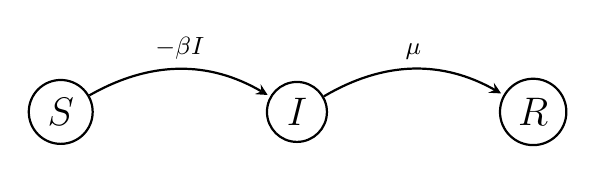
\begin{tikzpicture}[->,>=stealth,shorten >=1pt,auto,node distance=3cm, thick,main node/.style={circle,draw,font=\sffamily\Large\bfseries}]

  \node[main node] (S) {$S$};
  \node[main node] (I) [right of=S] {$I$};
  \node[main node] (R) [right of=I] {$R$};

  \path[every node/.style={font=\sffamily\small}]
    (S) edge [bend left] node [above] {$-\beta I$} (I)
    (I) edge [bend left] node [above] {$\mu$} (R);
\end{tikzpicture}
\]

A key difference with the work of Bernoulli is that the {\it force of infection:} $\beta I(t)$ (the rate at which susceptible individuals contract the disease) is not fixed in time, but proportional to the amount of people infected in the population. This is typical for human-human transmitted diseases in a well mixed population, where the probability of getting infected depends on the chances of meeting an infectious individual. This probability is proportional to the current amount of individuals in that state.

The dynamic variables for this model are:
\begin{itemize}
 \item $S(t)$, the fraction of the population susceptible to contracting the disease
 \item $I(t)$ the fraction that is currently infected and infectious
 \item $R(t) = 1- S(t)  - I(t)$ the fraction that is recovered or deceased.
\end{itemize}

We can write down the master equation of the stochastic process, which defines the evolution in time of $P_{S,I}(t)$, as
\[ \frac{\ud P_{S,I}(t)}{\ud t}  = \beta P_{S+1,I-1}(t) + \mu P_{S,I+1}(t) -\beta P_{S,I}(t) -\mu P_{S,I}(t)\]
By taking the average $S(t)= \frac 1 N \sum_{S,I} S P_{S,I}(t)$ and $I(t)= \frac 1 N \sum_{S,I} I P_{S,I}(t)$, we can obtain the deterministic version of this stochastic process, which characterize the evolution in time of the mean values:
\begin{eqnarray}
\frac{\ud S}{\ud t} &=& -\beta SI  \nonumber \\
\frac{\ud I}{\ud t} &=& \beta SI - \mu I  \label{eq:SIR} \\
\frac{\ud R}{\ud t} &=& \mu I \nonumber
\end{eqnarray}
where, the parameters
\begin{itemize}
 \item $\beta$ is the transmission rate or the rate at which susceptible individuals become infected.
\item $\mu$ is the recovery rate or the rate at which infected individuals recover and become immune.
\end{itemize}

The first equation describes the rate at which susceptible individuals become infected. It assumes that the rate of transmission is proportional to the product of the number of susceptible individuals and the number of infectious individuals, with the proportionality constant $\beta$.

The second equation describes the rate at which infected individuals recover. It assumes that the rate of recovery is proportional to the number of infectious individuals, with the proportionality constant $\mu$. The term $\beta SI$ represents the rate at which susceptible individuals become infected, and the term $\mu I$ represents the rate at which infected individuals recover.

The third equation describes the rate at which individuals recover from the disease and become immune. It assumes that the rate of recovery is proportional to the number of infectious individuals, with the proportionality constant $\mu$.

Sometimes, the equations are written in terms of populations instead of probabilities. You can obtain one from the other by multiplying (dividing) by the population size $N$:
\begin{eqnarray}
\frac{\ud S}{\ud t} &=& -\beta \frac I N S   \nonumber \\
\frac{\ud I}{\ud t} &=& \beta \frac S N I - \mu I  \label{eq:SIR} \\
\frac{\ud R}{\ud t} &=& \mu I \nonumber
\end{eqnarray}
In this case, $\frac  I N$ and $\frac S N$ can be interpreted as the density of infectious/susceptibles individuals, and $\beta$ is still the rate of transmssion contacts per unit time. The {\it force of infection} of a disease is the rate at which susceptible individuals become infected. Said differently, is the probability per unit time of a helathy individual of contracting the disease. In transmissible diseases will be $\beta \frac I N$ and it depends on the size of the infectious population.

These equations are a set of coupled first-order ordinary NON-LINEAR differential equations, which means that the values of $S$, $I$, and $R$ change over time according to the values of $\beta$, $\mu$, and the initial conditions. The nonlinearity, of course, causes some complications.

First epidemics models, however, were linear. For instance, if a model studies a disease that apperas in the population at a fixed rate, lets say, skin cancer (non transmissible), then a deterministic model looks like:
\begin{eqnarray}
 \frac{\ud S}{\ud t} &=& b S -\beta S -d S  \nonumber \\
\frac{\ud I}{\ud t} &=& \beta S - \mu I  -d_I I\label{eq:SIRlinear} \\
\frac{\ud R}{\ud t} &=& \mu I - d_R R \nonumber
\end{eqnarray}
Notice that this equations are linear, therefore an scaling by $N$ or any other factors is irrelevant.



\subsection{Deterministic epidemics from master equation}

Previous deterministic equations are similar in spirit to the master equation, but actually simpler and quite different in nature. While the stochasti process needs a full description of the probabilities of every possible state of the system, the SIR equations describe determinisic mean values of this process. Intuitively, following the law of large numbers, one expect that such large epidemics will be better described by the deterministic case.

Let us show how deterministic equations are obtained by averaging the master equation. Consider the SIR epidemic process. The full space of the stochastic process is given by the dots in the figure, laying in the area $S+I\leq N$.
\[
\begin{tikzpicture}[scale=0.5]
  \draw[->] (-1,0) -- (21,0) node[right] {$S$};
  \draw[->] (0,-1) -- (0,21) node[above] {$I$};
  \foreach \x in {0,2,...,20}
    {\tikzmath{\maxy = 20-\x;}
    \foreach \y in {0,2,...,\maxy}
      \filldraw[black] (\x,\y) circle (2pt);}
  \draw[->, ultra thick, red] (10,4) -- (8,6);
  \draw[->, ultra thick, green] (10,4) -- (10,2);
  \draw[->, thick,dashed, red] (12,2) -- (10.5,3.5);
  \draw[->, thick,dashed, green] (10,6) -- (10,4.5);
  \draw[dashed] (0,20) -- (20,0);
\end{tikzpicture} \]
The red arrow exemplifies the contagion process, and the green arrow the recovery process. So, from any given state $(S,I)$ there are two possible transitions
\begin{eqnarray*}
 (S , I) &\xrightarrow{W_{I}}& (S-1,I+1) \qquad (S,I) \xrightarrow{W_R} (S,I-1)  \\
\end{eqnarray*}
with transition rates given by
\[W_{I} = \beta \frac I N S  \qquad W_{R} = \mu I\]
The master equations reads
\[ \frac{\ud P_t(S,I)}{\ud t} = \beta  \frac {I-1} N (S+1) P_t(S+1,I-1) +  \mu (I+1) P_t(S,I+1) - \beta  \frac {I} N {S} P_t(S,I) -  \mu (I+1) P_t(S,I)\]
Multiplying by $S$ and tracing over $S$ and  $I$
\begin{eqnarray*}
 \frac{\ud \langle S \rangle}{\ud t} &=& \beta  \sum_{S,I} \frac {I-1} N S (S+1) P_t(S+1,I-1) +  \mu \sum_{S,I}  S (I+1) P_t(S,I+1) - \\
 && - \beta  \sum_{S,I} \frac {I} N {S^2} P_t(S,I) -  \mu\sum_{S,I}  S I P_t(S,I)
\end{eqnarray*}
It suffices to assume that $P(S,I)\equiv 0$ whenever either of the arguments is negative or $S+I>N$, to change variables and obtain:
\begin{eqnarray*}
 \frac{\ud \langle S \rangle}{\ud t} &=& \beta  \sum_{\tilde S,\tilde I} \frac {I} N (S-1) S P_t(S,I) +  \mu \sum_{S,\tilde I}  S I P_t(S,I) - \\
 && - \beta  \sum_{S,I} \frac {I} N {S^2} P_t(S,I) -  \mu\sum_{S,I}  S I P_t(S,I) \\
 &=& - \beta \frac 1 N \langle S I \rangle
\end{eqnarray*}

Repeating for the average of $I$, we get the equations
\begin{eqnarray*}
 \frac{\ud \langle S \rangle}{\ud t}  &=& - \beta \frac 1 N \langle S I \rangle \\
  \frac{\ud \langle I \rangle}{\ud t}  &=& + \beta \frac 1 N \langle S I \rangle - \mu \langle I\rangle
\end{eqnarray*}
which are similar but yet not the same as the SIR model equations. A further assumption $\langle S I \rangle \simeq \langle S \rangle  \langle I \rangle $ is required to reproduce SIR model. This assumption shall be good if the variables S and I are actually independent, which is not mathematically the case. But it shall be a good approximation is the distribution $P_t(S,I)$ is sharply picked arround its mean values. This is the case for large systems, where we expect a sort of law of large numbers to concentrate the stochastic process on its typical values.


\subsection{Short time limit}

In the early stages of an epidemic, when the number of infected individuals is small compared to the total population size, the SIR model can be approximated by a linear differential equation. %This linearized SIR model predicts that the number of infected individuals grows exponentially at a rate proportional to the number of susceptible individuals, until a significant proportion of the population becomes infected and the epidemic enters a saturation phase.
Suppose that the initial number of infected individuals is small compared to the total population size, i.e., $I(0) \sim 1/N$, where $N$ is the total population size. Then, the number of susceptible individuals can be approximated as $S(t) \simeq 1$, and the number of recovered individuals can be approximated as $R(t) \sim 1/N$.

Under these assumptions, the dynamics of the infected compartment can be approximated by the following linear differential equation:
\begin{equation}
    \frac{dI}{dt} = \beta S(t) I(t) - \mu I(t),
\end{equation}
where $\beta$ is the transmission rate, $\mu$ is the recovery rate, and $I(t)$ is the fraction of infected individuals at time $t$. During the initial epidemic phase, when few cases still exists compared to the population size, we can approximate $S(t) = S(0) = 1$, and write the linear equation:
\begin{equation}
    \frac{dI}{dt} = \lambda I(t), \qquad \mbox{where }   \lambda = \beta - \mu.
\end{equation}
The solution to this linear differential equation is an exponential function of the form:
\begin{equation}
    I(t) = I(0) \exp(\lambda t).
\end{equation}
The exponential solution of the SIR model in the low prevalence linear phase shows that the number of infected individuals changes exponentially, growing when $\beta>\mu$, and decreasing when $\beta<\mu$.  This exponential growth phase is characteristic of the beginning of an epidemic, when the number of infected individuals is small compared to the total population size and the epidemic has not yet reached a significant proportion of the population. 

The basic reproduction number $R_0$, is the expected number of new infections created by every single infected individual, in the early exponential phase of an epidemic. Since $\mu$ is the recovery rate, $\tau = 1/\mu$ is the expected duration of the infection on an individual. Since $\beta$ is the rate of new cases, $R_0 = \beta \tau = \beta/\mu$ is the average number of new cases created by an infected individual during the period in which it is actively infectious. Notice that the criteria $\lambda \lessgtr 0$ is equivalent to $R_0 \lessgtr 1$.

%The duration and magnitude of the exponential growth phase depend on the initial conditions and the parameters of the model, such as the transmission rate and recovery rate.

\subsection{Infinite time limit}

Properties of SIR equations. Since the total amount of studied subjects remain invariant, only their categories changes, $S(t)+I(t)+R(t) =1$. This can also be proven by adding (\ref{eq:SIR}). Furthermore, since \[ S'(t)+I'(t) = -\mu I(t)\] is a decreasing non negative function, it converges to a limit $S_\infty + I_\infty$ in $t\to\infty$. Moreover, it is easy to see that $I_\infty$ can only be zero, so $S+I \to S_\infty$.

Integration of the previous equation results in
\[ 1 - S_\infty  = \mu \int_0^\infty I(t)\ud t
\]
The first number $S_0+I_0 = 1$ comes from assuming that all the population is originally in the states S or I.

Dividing the equation for $S'(t)$ by $S(t)$, we get
\[ \frac{ \ud \log S(t)}{\ud t}  =  -\beta I(t) \quad \mbox{that integrating }\quad  \log(S_\infty / S_0) = -\beta \int_0^\infty I(t)\ud t\] This results in a relation for the final amount of susceptible individuals
\[\log(S_0 / S_\infty)  = \frac \beta \mu (1-S_\infty) = R_0 (1-S_\infty) \]
that is called the {\it final size relation} for the epidemic. If the variables are kept extensive $\tilde S(t) = N S(t), \tilde I(t) \ldots $, the final relation reads
\begin{equation}
 \log(\tilde S_0 / \tilde S_\infty)  =  R_0 (1-\frac {\tilde S_\infty} N) \label{eq:Sinf} 
\end{equation}
which is a useful relation between the basic reproduction number and the final size of the epidemic. 

The total number of infected people in the population is given by $N-\tilde S_\infty$, and the fraction $1-S_\infty$ or $1-\frac {\tilde S_\infty }N$ is called the {\it attack rate}, although it is not a rate, but a fraction.

Another conclusion from (\ref{eq:Sinf}) is that $S_\infty>0$, and so, in every epidemic there is always a fraction of the population that will not be infected.

While the recovery rate $\mu$ is generally simple to estimate from studies on infected individuals. However the contact rate $\tilde \beta = \beta/N$ is much harder. Direct calculation of $\beta$, or of $R_0 =\beta/\mu$ can be difficult, while a post facto analysis of the epidemic through serological studies, can provide estimation for $S_\infty$, and through (\ref{eq:Sinf}), to $R_0$ and $\beta$.

\[
   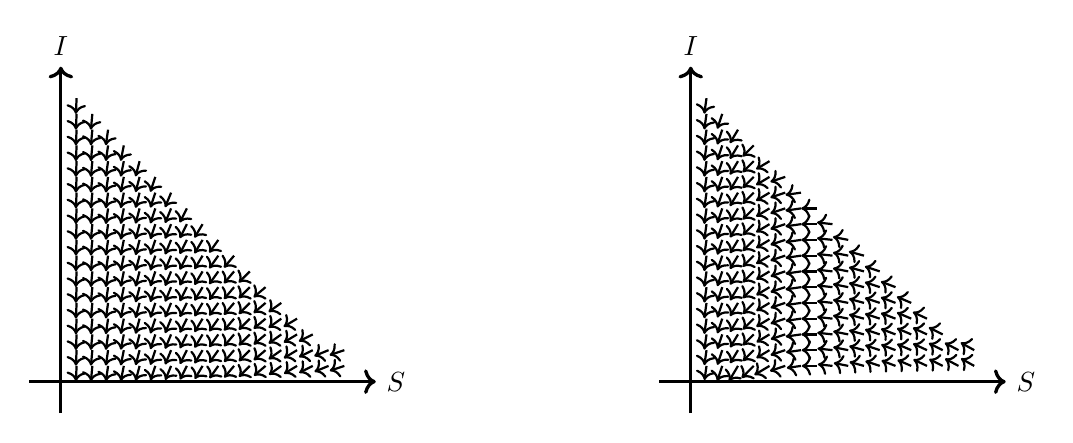
\begin{tikzpicture}[
    scale=4,
    axis/.style={very thick, ->},
    important line/.style={thick},
    dashed line/.style={dashed, thin},
    pile/.style={thick, ->, shorten <=2pt, shorten
    >=2pt},
    every node/.style={color=black}
    ]
        % Draw grid
%        \draw[step=0.2,gray,thin] (0,0) rectangle (1,1);
%        \draw[thick,->] (0,0) -- (3.1,0) node[anchor=north west] {X};
%        \draw[thick,->] (0,0) -- (0,3.1) node[anchor=south east] {Y};
          \draw[axis] (-0.1,0)  -- (1.0,0) node(xline)[right] {$S$};
        \draw[axis] (0,-0.1) -- (0,1.0) node(yline)[above] {$I$};
        %\draw[thick] (0,0) rectangle (1,1);        % Draw vectors
        \foreach \x in {0.05,0.1,...,0.95}
            {\tikzmath{\e = 1.0-\x;}
            \foreach \y in {0.05,0.1,...,\e}
            {
                  \tikzmath{\dx = -0.5* \x * \y;
                            \dy =  -1* \dx -0.6* \y;
                             \norm = {sqrt(100*\dx*\dx + 100*\dy*\dy)};
                             \dxn = 10*0.05*\dx/(0.01+\norm);
                             \dyn = 10*0.05*\dy/(0.01+\norm);
                            }
                  \draw[->,thick] (\x,\y) -- ( \x+\dxn, \y+\dyn );}}
          \draw[axis] (1.9,0)  -- (3.0,0) node(xline)[right] {$S$};
        \draw[axis] (2.0,-0.1) -- (2.0,1.0) node(yline)[above] {$I$};
        %\draw[thick] (0,0) rectangle (1,1);        % Draw vectors
        \foreach \x in {0.05,0.1,...,0.95}
            {\tikzmath{\e = 1.0-\x;}
            \foreach \y in {0.05,0.1,...,\e}
            {
                  \tikzmath{\dx = -0.5* \x * \y;
                            \dy =  -1* \dx -0.2* \y;
                             \norm = {sqrt(100*\dx*\dx + 100*\dy*\dy)};
                             \dxn = 10*0.05*\dx/(0.01+\norm);
                             \dyn = 10*0.05*\dy/(0.01+\norm);
                            }
                  \draw[->,thick] (2+\x,\y) -- ( 2+\x+\dxn, \y+\dyn );}}
                  
\end{tikzpicture}
\]

A similar procedure as the one we carried, but taken up to time $t$ instead of $\infty$, results in a parametric relation between $S(t)$ and $I(t)$:
\begin{equation} 
I(t) +S(t) - \frac \mu\beta \log S(t) = 1- \frac \mu\beta \log S_0 \label{eq:SIintime}
\end{equation}

This trajectories correspond to the flux lines in the diagram of $I$ vs $S$, using the vector defined by the right hand side of (\ref{eq:SIR}), normalized.

The maximum number of infectives at any time is the number of infectives when the derivative of $I$ is zero, that is, when $S = \mu /\beta$ . This maximum is obtained by replacing this value into (\ref{eq:SIintime}) as
\[ I_{max} =  I_0 +S_0 - \frac \mu\beta \log S_0  - \frac \mu\beta +\frac \mu\beta \log \frac{\mu}{\beta} 
\]

\subsection{Epidemics terminology}

A clear definition of terms is essential for the correct handling of epidemics. At the onset of any epidemic and in particular for emerging diseases, a clear statement of what is going to be consider a ``case'', a ``death caused by the disease'', a primary or secondary case, among others, is essential for a meaningful collection of statistical data, which is a key aspect of epidemiology.

Following WHO summary of terms for COVID (COVID-19, GLOSSARY: OUTBREAKS AND EPIDEMICS, A resource for journalists and communicators), here comes a selected list of useful terms related to epidemics:
\begin{itemize}
\item Emerging disease: An unknown or newly appeared disease, usually of the infectious or communicable type.
\item Reemerging disease: Resurgence or increase in the incidence of infectious or
communicable diseases that were considered to be already under control.
\item Seasonality of disease: Regular pattern of variation in the occurrence of some diseases
(for example, the flu) during different seasons of the year.
\item Incidence: The number of new cases of a disease in a population in a given period.
Incidence measures the speed at which new cases occur during a given period in a specific
population—for example, the number of new cases of HIV infection in gay men in a country in 2019.
 \item Prevalence: The total number of people who have a disease (new and existing cases)
in a population or in a given place at a given time. Prevalence is an indicator of the
magnitude of a disease—for example, the total number of people with tuberculosis in
a country in 2019. Incidence and prevalence are essentially different ways of measuring
the frequency of disease. The relationship between them varies from disease to disease.
\item Attack rate: Number of people who contract a disease out of the entire group of people exposed to the disease. Expressed as a percentage.
\item Agent: A microorganism, chemical substance, or form of radiation whose
presence, excessive presence, or relative absence is essential for the occurrence of
a disease Agents may be biological (living organisms, such as viruses and bacteria) and
non-biological (chemicals, such as pesticides, and physical phenomena, such as radiation).
\item Case-fatality rate: The percentage of people affected by a disease or a particular event who die in a given period. Frequently used to describe the severity of an epidemic.
\item Contact: A person who has been in contact with an infected person (case) such that he/she is considered to have had significant exposure and is therefore at risk of infection.
\item Contagious or infectious: Terms that are often used interchangeably but that have subtle differences in meaning. “Contagious” is related to direct or indirect spread from person to person. The flu, for example, is very contagious, but Ebola is not. “Infectious” means that contact with a small amount of virus can cause disease. Ebola, for example, is very infectious.
\item Host: A person or other living animal, including birds and arthropods, that affords
subsistence or lodgment to an infectious agent under natural conditions.
\item Exposure: Contact with an infectious agent or a risk factor that can cause a disease.
Exposure has two dimensions: degree or level, and duration.
\item Incidence rate: Rate of new cases in a population. The numerator is the number of
new events that they occur in a given period. The denominator is the population at risk of
experiencing the event of interest during this period.
\item Infectious period: Period of time during which a person can transmit a disease. This period may precede the onset of symptoms and may last longer than the symptoms.
\item Latent period: Time that elapses from exposure to an agent until the date that
a person can transmit a disease (this is the period that immediately precedes the
infectious period).
\item Mortality rate: Percentage of people in a population who die out of the total
population. May be expressed per 100, 1,000, or another number.
\item Virulence: The ability of an infectious agent to produce severe and fatal cases. The measure of virulence is the ratio of the number of severe and fatal cases to total overt cases.
\item Basic reproduction number (R0): The spread of a disease in a population (especially in epidemics) depends on the basic reproduction number (or R0) and the generation time (usually established on the basis of the serial interval). The R0 is the number of people to whom an
infected person can transmit the disease or the number of secondary cases that each
primary case generates on average (during the contagious period).
\item Generation time: the time between the  onset of infection in the primary case and the
onset of infection in a secondary case (i.e., a case infected by the primary case)
\item Serial interval: In practical terms, this is the time between the onset of the disease
in the primary case and the onset of the disease in the secondary case: the longer the serial interval, the more time there is to act on the problem, implement prevention and control measures, and, therefore, the better the chances of containing the epidemic.
The shorter the generation time, the more difficult it is to control the outbreak.
\item Isolation means separating sick or infected people from others to prevent infection from
spreading.
\item Quarantine means restricting the movement of healthy people who may have
been exposed to a virus but are not sick.
\item Herd immunity: Indirect protection against disease that results from a sufficient number
of individuals in a community having immunity to that disease. With enough immune individuals, the transmission of a disease can be reduced, thus limiting the potential for any one individual to be exposed to it. Generally, PAHO recommends vaccination coverage of $95\%$ or more to ensure herd immunity. Herd immunity does not apply to diseases such as tetanus that are
not spread via person-to-person contact.
\end{itemize}

\section{SIS model and epidemic thresholds}

SIR epidemics mimic diseases that generate immunity, that is, that you can not take twice. This is the case of many (most) diseases, but it is not the case of many others, as, typically, sexually transmitted diseases, as clamydia and gonorrhea. This diseases are actually best represented by SIS types of models. These are characterized by the transitions
\begin{eqnarray*}
 S + I &\xrightarrow{\beta}& 2I \\
 I &\xrightarrow{\mu}& S \\
\end{eqnarray*}
and the corresponding determinisic equations
\begin{eqnarray}
\frac{\ud S}{\ud t} &=& -\beta SI   + \mu I\nonumber \\
\frac{\ud I}{\ud t} &=& \beta SI - \mu I  \label{eq:SIS}
\end{eqnarray}
While the epidemic phase $I > 0$ in an SIR model last a finite period of time, recurrent diseases can sustain epidemics for infinite time, normally referred as endemic phase. While SIS model is also non linear, the steady state can be easily deduced by setting to zero the time derivatives:
\begin{eqnarray}
\frac{\ud S}{\ud t}\equiv 0 &=& -\beta SI   + \mu I\nonumber \\
\frac{\ud I}{\ud t}\equiv  0  &=& \beta SI - \mu I  \label{eq:SIS}
\end{eqnarray}
resulting in the equilibrium solution
\[ S_{eq} = \frac \mu  \beta \qquad  I_{eq} = 1-S_{eq} = \frac{\beta - \mu } \beta\]
Of course this values will be meaningful if they are in the $[0,1]$ range, meaning that only the case $\beta > \mu$ will generate an endemic phase.
The value $\beta / \mu = 1$, corresponding also with $R_0=1$, defines the threshold above/below which endemic states do/do not exist.

Sometimes, SIS is a too simplistic approach, since almost every disease generates some level of immunity, although it can be lost in time.

\section{And beyond}

Reasons why deterministic description of epidemics is a very narrow approach:
\begin{itemize}
 \item Well mixed systems are non realistic. Human behavior is a mixture of repetitive patterns (go to school, visit your parents, etc) and random interactions (in the public transport system), also influenced by distance constraints. The network of human contacts is best modelled by a dynamic network with rather stable clusterized subnetworks and random links whose probability decays with distance.
 \item Fluctuations: as the whole approach relies implicitly in the law of large numbers, fluctuations are completely ignored. Epidemic processes like SIS  have an absorbing state, i.e. $I=0$. Even epidemics above the epidemic threshold can be suppressed by fluctuations.
 \item Implies memorlyless processes. The assumption that recovery times follow an exponential distribution is motivated by its mathematical convenience rather than its epidemiological plausibility.
\end{itemize}



\section{Homework}

\begin{enumerate}

 \item  Find out the incidence in a year and the prevalence of HIV in Cuba, China, India, USA, Haiti, Nigeria, Spain.

\item Consider the linear model in (\ref{eq:SIRlinear}) as a model for skin cancer.
\begin{enumerate}
 \item What are reasonable values for the constants $b$ and $d$?
 \item Assume that half of people with skin cancer get cure, and half die of this condition. What can we say about $\mu$ and $d_I$?
 \item Force of infection (not actually infection, but developing the disease), lets say is $\beta = 10^{-4}$. And for those who die of this disease, the average time from contraction to death is 1 year. Compute how many individuals are currently living with skin cancer.
 \end{enumerate}

 \item Show that the number of infectious individuals always go to zero in the long time limit of the SIR model.

 \item Consider $\theta  = \beta / \mu$ and using
 \[ I = N -R-S_0 e^{-\theta R(t)}\]
 show that the maximum number of infectious people occurs exactly at $S(t)= 1/\theta$. Show also that in the long time limit not everybody was infected. {\bf Comment:} The first result can be derived in many different ways, some easier than the one proposed.

 \end{enumerate}

 \chapter{Introduction to networks}

\textbf{Definition:} A \textit{graph} $G$ is a pair $(V, E)$, where $V$ is a set of vertices (or nodes), and $E$ is a set of edges, where each edge is a pair of vertices $(u, v) \in V \times V$. 
\begin{itemize}
 \item The vertices are said to be adjacent if they are endpoints of an edge. 
 \item The set of all edges incident to a vertex $v$ is called the \textit{neighborhood} of $v$, denoted by $\partial v$.
\end{itemize}
 

The \textit{adjacency matrix} $A_G$ of a graph $G$ is:
\begin{itemize}
 \item a square matrix of size $n \times n$, where $n = |V|$,
 \item if $(u,v)\in E$, then $A_G(u,v) = 1 $ 
 \item else $A_G(u,v) = 0 $
\end{itemize}


Consider the graph $G = (V, E)$, where $V = \{1,2,3,4\}$ and \[E = \{(1,2),(1,3),(2,3),(3,4)\}\]. The graph $G$ and its adjacency matrix $A_G$ are shown below:

\[
G = 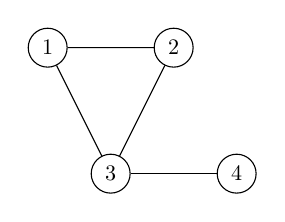
\begin{tikzpicture}[scale=0.8, transform shape]
    \node[shape=circle,draw=black] (1) at (0,2) {1};
    \node[shape=circle,draw=black] (2) at (2,2) {2};
    \node[shape=circle,draw=black] (3) at (1,0) {3};
    \node[shape=circle,draw=black] (4) at (3,0) {4};
    \draw[-] (1) -- (2);
    \draw[-] (1) -- (3);
    \draw[-] (2) -- (3);
    \draw[-] (3) -- (4);
\end{tikzpicture} \qquad A_G = \begin{bmatrix}
0 & 1 & 1 & 0 \\
1 & 0 & 1 & 0 \\
1 & 1 & 0 & 1 \\
0 & 0 & 1 & 0
\end{bmatrix}
\]


%In the adjacency matrix $A_G$, the entry $A_G(i,j)$ is 1 if there is an edge between vertices $i$ and $j$ in the graph $G$, and 0 otherwise. For example, $A_G(1,2) = 1$, since there is an edge between vertices 1 and 2 in the graph $G$.

\textbf{Degree of a Node:} The \textit{degree} of a node $v$ in a graph $G = (V,E)$ is the number of edges incident to $v$, i.e., the number of neighbors of $v$. The degree of $v$ is denoted by $deg(v)$. In a directed graph, the degree of a node is the sum of its in-degree (number of incoming edges) and out-degree (number of outgoing edges).

\textbf{Neighborhood of a Node:} The \textit{neighborhood} of a node $v$ in a graph $G = (V,E)$ is the set of all nodes that are adjacent to $v$, i.e., the set of all neighbors of $v$. The neighborhood of $v$ is denoted by $\partial_v$.

For example, in the previous graph, the degree of node 1 is 2, since it has 2 neighbors (nodes 2 and 3), i.e., $deg(1) = 2$. Similarly, the degree of node 2 is 2 and the degree of node 3 is 3. The degree of node 4 is 1, since it has only 1 neighbor (node 3).

The neighborhood of node 1 is $\partial_1 = \{2, 3\}$, since nodes 2 and 3 are adjacent to node 1. Similarly, the neighborhood of node 2 is $\partial_2 = \{1, 3\}$, the neighborhood of node 3 is $\partial_3 = \{1, 2, 4\}$, and the neighborhood of node 4 is $\partial_4 = \{3\}$.

The adjacency matrix can be used to compute various properties of the graph, such as the number of paths of a certain length between two vertices, the number of cycles of a certain length in the graph, and many others.


\textbf{Paths:} A \textit{path} in a graph $G=(V,E)$ is a sequence of distinct vertices $v_1, v_2, \ldots, v_k$ such that $(v_i, v_{i+1}) \in E$ for $i=1,2,\ldots,k-1$. The length of the path is $k-1$, and it is denoted by $|P|$. A path is said to be \textit{simple} if all its vertices are distinct.

\textbf{Cycles:} A \textit{cycle} in a graph $G=(V,E)$ is a simple path $v_1, v_2, \ldots, v_k$ such that $(v_k, v_1) \in E$. The length of the cycle is $k$, and it is denoted by $|C|$.

\textbf{Adjacency Matrix and Paths:} The adjacency matrix $A_G$ of a graph $G$ can be used to compute the number of paths between two nodes $u$ and $v$ in the graph. The entry $(A_G)^n(u,v)$ gives the number of paths of length $n$ between nodes $u$ and $v$. Specifically, the $(u,v)$ entry of $A_G^n$ gives the number of paths of length $n$ from node $u$ to node $v$.

To see why this is true, consider the $(u,v)$ entry of $A_G^2$. This entry is given by $(A_G^2)_{u,v} = \sum_{w \in V} A_G(u,w) A_G(w,v)$, which counts the number of paths of length 2 from $u$ to $v$ by summing over all possible intermediate nodes $w$. By induction, we can show that $(A_G)^n(u,v)$ counts the number of paths of length $n$ between nodes $u$ and $v$.

In the previous graph, to compute the number of paths of length 2 between nodes 1 and 4, we can compute $(A_G)^2(1,4)$, which is equal to $[(A_G)^2]_{1,4} = A_G(1,2)A_G(2,3) + A_G(1,3)A_G(3,4) = 1 \cdot 1 + 1 \cdot 1 = 2$. Therefore, there are two paths of length 2 between nodes 1 and 4 in the graph $G$.

The adjacency matrix of a graph $G$ can also be used to compute the number of cycles of a certain length $k$ in the graph. Specifically, the $(i,j)$ entry of the matrix $A_G^k$ gives the number of cycles of length $k$ that contain the edge $(i,j)$.

To see why this is true, consider the $(i,j)$ entry of $A_G^k$. This entry is given by $(A_G^k)_{i,j} = \sum_{w_1, w_2, \ldots, w_{k-1}} A_G(i,w_1) A_G(w_1,w_2) \cdots A_G(w_{k-1},j)$, which counts the number of paths of length $k$ from $i$ to $j$ by summing over all possible intermediate nodes $w_1, w_2, \ldots, w_{k-1}$. If the edge $(i,j)$ is part of a cycle of length $k$, then we have $w_1, w_2, \ldots, w_{k-1} \neq i,j$ and the last term $A_G(w_{k-1},j)$ in the sum will be equal to 1 (since $(w_{k-1}, j)$ is an edge in the cycle), while all other terms in the sum will be nonzero. Therefore, the $(i,j)$ entry of $A_G^k$ will count the number of cycles of length $k$ that contain the edge $(i,j)$.

For example, let's consider the following graph $G$:

\[
G = 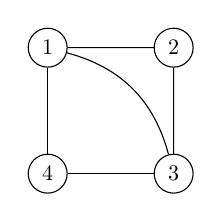
\begin{tikzpicture}[scale=0.8, transform shape]
    \node[shape=circle,draw=black] (1) at (0,2) {1};
    \node[shape=circle,draw=black] (2) at (2,2) {2};
    \node[shape=circle,draw=black] (3) at (2,0) {3};
    \node[shape=circle,draw=black] (4) at (0,0) {4};
    \draw[-] (1) -- (2);
    \draw[-] (2) -- (3);
    \draw[-] (3) -- (4);
    \draw[-] (4) -- (1);
    \draw[-] (1) to [bend left=30] (3);
\end{tikzpicture}
\]

The adjacency matrix of $G$ is:

\[
A_G = \begin{bmatrix}
0 & 1 & 0 & 1 \\
1 & 0 & 1 & 0 \\
0 & 1 & 0 & 1 \\
1 & 0 & 1 & 0
\end{bmatrix}
\]

To compute the number of cycles of length 3 in the graph $G$, we can compute the matrix $A_G^3$ and count the number of entries that are nonzero. Since we are interested in cycles of length 3, we only need to consider the entries of $A_G^3$ that correspond to edges in the graph $G$. For example, the entry $(1,2)$ of $A_G^3$ gives the number of cycles of length 3 that contain the edge $(1,2)$. We have:

\begin{align*}
(A_G^3)_{1,2} &= \sum_{w_1, w_2} A_G(1,w_1) A_G(w_1,w_2) A_G(w_2,2) \\
&= A_G(1,4) A_G(4,3) A_G(3,2) \\
&= 1 \cdot 1 \cdot 1 \\
&= 1
\end{align*}

Therefore, there is exactly one cycle of length 3 in the graph $G$ that contains the edge $(1,2)$. Similarly, we can compute the other entries of $A_G^3$ to count the number of cycles of length 3 that contain the other edges in the graph. In this case, we find that there are three cycles of length 3 in the graph $G$.

\section{Directed graphs}

No problem, here's a directed version of the graph you requested:

\[
G = 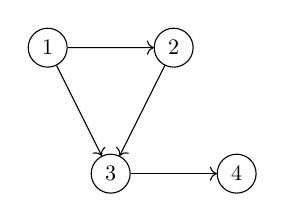
\begin{tikzpicture}[->, scale=0.8, transform shape]
\node[shape=circle,draw=black] (1) at (0,2) {1};
\node[shape=circle,draw=black] (2) at (2,2) {2};
\node[shape=circle,draw=black] (3) at (1,0) {3};
\node[shape=circle,draw=black] (4) at (3,0) {4};
\draw[->] (1) -- (2);
\draw[->] (1) -- (3);
\draw[->] (2) -- (3);
\draw[->] (3) -- (4);
\end{tikzpicture}
\]

The adjacency matrix of $G$ is:

\[
A_G = \begin{bmatrix}
0 & 1 & 1 & 0 \\
0 & 0 & 1 & 0 \\
0 & 0 & 0 & 1 \\
0 & 0 & 0 & 0
\end{bmatrix}
\]

To compute the in-degree and out-degree of each vertex in the graph $G$, we can sum the entries of the corresponding rows and columns in the adjacency matrix. We have:

\begin{itemize}
  \item Vertex 1: in-degree = 0, out-degree = 2
  \item Vertex 2: in-degree = 1, out-degree = 1
  \item Vertex 3: in-degree = 2, out-degree = 1
  \item Vertex 4: in-degree = 1, out-degree = 0
\end{itemize}

In this case, vertex 1 and vertex 4 are sources and sink, respectively.

\section{Wheigted graphs}

A weighted graph is a graph where each edge has a numerical value associated with it, called a weight. The weight often represents some sort of cost, distance, or importance associated with traversing the edge.

In mathematical terms, a weighted graph is represented by a graph $G = (V, E, w)$, where $V$ is the set of vertices (nodes), $E$ is the set of edges, and $w :  E \rightarrow \mathbb{R}$ is a function that assigns a weight to each edge.

\[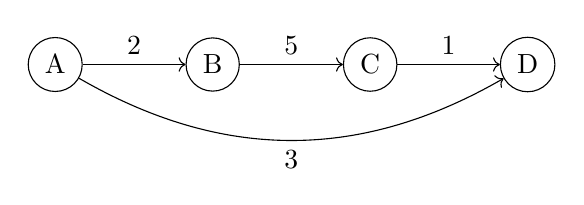
\begin{tikzpicture}
  \node[circle, draw] (A) at (0,0) {A};
  \node[circle, draw] (B) at (2,0) {B};
  \node[circle, draw] (C) at (4,0) {C};
  \node[circle, draw] (D) at (6,0) {D};
  \draw[->] (A) -- node[above] {2} (B);
  \draw[->] (B) -- node[above] {5} (C);
  \draw[->] (C) -- node[above] {1} (D);
  \draw[->] (A) to[bend right] node[below] {3} (D);
\end{tikzpicture}\]
In this example, we define a weighted graph with four nodes (A, B, C, and D) and four edges with weights (2, 5, 1, and 3). 
In this graph, the weights on the edges represent the cost or distance associated with traversing the edge. For example, to get from node A to node D, we could either take the edge with weight 2 and the edge with weight 1, or we could take the edge with weight 3. The choice of which path to take would depend on the specific application of the graph.

\section{Graphs properties}

1. {\bf Connected vs Disconnected Graphs}: A connected graph is a graph where there is a path between any two vertices in the graph. A disconnected graph is a graph that is not connected, meaning that there are at least two vertices that are not connected by a path. For example, the following graph is connected:

\[
G = 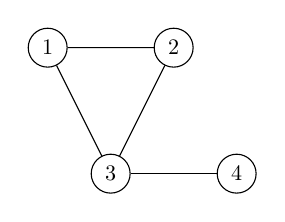
\begin{tikzpicture}[scale=0.8, transform shape]
\node[shape=circle,draw=black] (1) at (0,2) {1};
\node[shape=circle,draw=black] (2) at (2,2) {2};
\node[shape=circle,draw=black] (3) at (1,0) {3};
\node[shape=circle,draw=black] (4) at (3,0) {4};
\draw[-] (1) -- (2);
\draw[-] (1) -- (3);
\draw[-] (2) -- (3);
\draw[-] (3) -- (4);
\end{tikzpicture}
\]

while the following graph is disconnected:

\[
G = 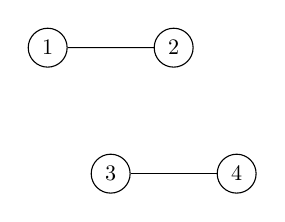
\begin{tikzpicture}[scale=0.8, transform shape]
\node[shape=circle,draw=black] (1) at (0,2) {1};
\node[shape=circle,draw=black] (2) at (2,2) {2};
\node[shape=circle,draw=black] (3) at (1,0) {3};
\node[shape=circle,draw=black] (4) at (3,0) {4};
\draw[-] (1) -- (2);
\draw[-] (3) -- (4);
\end{tikzpicture}
\]

2. {\bf Regular vs Non-Regular Graphs}: A regular graph is a graph where all vertices have the same degree, meaning that each vertex has the same number of neighbors. A non-regular graph is a graph where the degrees of the vertices are not all the same. For example, the following graph is regular:

\[
G = 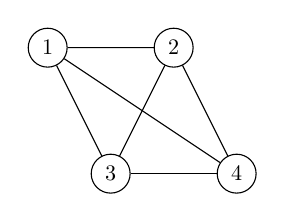
\begin{tikzpicture}[scale=0.8, transform shape]
\node[shape=circle,draw=black] (1) at (0,2) {1};
\node[shape=circle,draw=black] (2) at (2,2) {2};
\node[shape=circle,draw=black] (3) at (1,0) {3};
\node[shape=circle,draw=black] (4) at (3,0) {4};
\draw[-] (1) -- (2);
\draw[-] (1) -- (3);
\draw[-] (1) -- (4);
\draw[-] (2) -- (3);
\draw[-] (2) -- (4);
\draw[-] (3) -- (4);
\end{tikzpicture}
\]

while the following graph is non-regular:

\[
G = 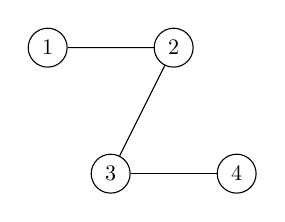
\begin{tikzpicture}[scale=0.8, transform shape]
\node[shape=circle,draw=black] (1) at (0,2) {1};
\node[shape=circle,draw=black] (2) at (2,2) {2};
\node[shape=circle,draw=black] (3) at (1,0) {3};
\node[shape=circle,draw=black] (4) at (3,0) {4};
\draw[-] (1) -- (2);
\draw[-] (2) -- (3);
\draw[-] (3) -- (4);
\end{tikzpicture}
\]

3. {\bf Planar vs Non-Planar Graphs:} A planar graph is a graph that can be drawn on a plane without any edges crossing. A non-planar graph is a graph that cannot be drawn on a plane without any edges crossing. For example, the following previous non regular graph is planar, while the following graph is non-planar:
\[
G = 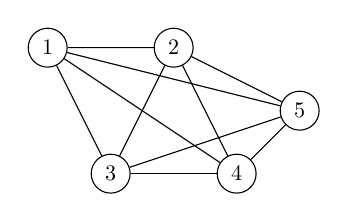
\begin{tikzpicture}[scale=0.8, transform shape]
\node[shape=circle,draw=black] (1) at (0,2) {1};
\node[shape=circle,draw=black] (2) at (2,2) {2};
\node[shape=circle,draw=black] (3) at (1,0) {3};
\node[shape=circle,draw=black] (4) at (3,0) {4};
\node[shape=circle,draw=black] (5) at (4,1) {5};
\draw[-] (1) -- (2);
\draw[-] (1) -- (3);
\draw[-] (2) -- (3);
\draw[-] (3) -- (4);
\draw[-] (4) -- (1);
\draw[-] (4) -- (5);
\draw[-] (4) -- (2);
\draw[-] (1) -- (5);
\draw[-] (2) -- (5);
\draw[-] (3) -- (5);
\end{tikzpicture}
\]
Less trivially, the previous example of a regular graph is also planar, although it doesn't seem so. Check that moving node 4 to the inside of the triangle created by the other three nodes, you can actually paint it without crossing lines.

4.{\bf Bipartite Graphs}: A bipartite graph is a graph where the vertices can be divided into two sets such that there is no edge between vertices in the same set. The previous example of a non-planar graph, is also a non-bipartite graph. On the contrary, the following graph is bipartite with sets $\{1,2\}$ and $\{3,4\}$:
\[
 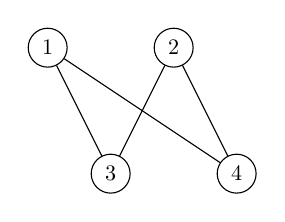
\begin{tikzpicture}[scale=0.8, transform shape]
\node[shape=circle,draw=black] (1) at (0,2) {1};
\node[shape=circle,draw=black] (2) at (2,2) {2};
\node[shape=circle,draw=black] (3) at (1,0) {3};
\node[shape=circle,draw=black] (4) at (3,0) {4};
\draw[-] (1) -- (3);
\draw[-] (1) -- (4);
\draw[-] (2) -- (3);
\draw[-] (2) -- (4);
\end{tikzpicture}
\]

5. {\bf Trees:} A tree is a connected graph with no cycles, meaning that there is exactly one path between any two vertices in the graph. For example, the following graph is a tree:
\[
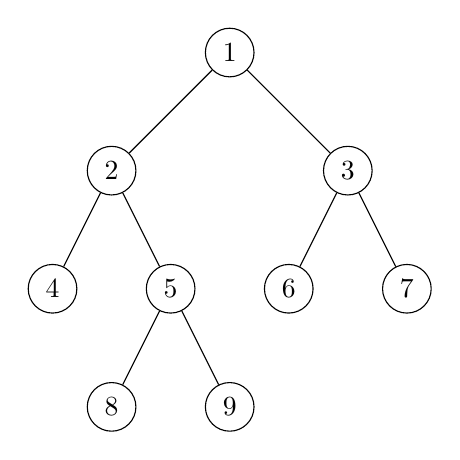
\begin{tikzpicture}[level distance=1.5cm,
  level 1/.style={sibling distance=3cm},
  level 2/.style={sibling distance=1.5cm}]
  \node[circle,draw](1){$1$}
    child{node[circle,draw](2){$2$}
      child{node[circle,draw](4){$4$}}
      child{node[circle,draw](5){$5$}
        child{node[circle,draw](8){$8$}}
        child{node[circle,draw](9){$9$}}
      }
    }
    child{node[circle,draw](3){$3$}
      child{node[circle,draw](6){$6$}}
      child{node[circle,draw](7){$7$}}
    };
\end{tikzpicture}\]

Trees are important in many applications, such as in computer science where they are used to represent hierarchical structures like file systems or organization charts.

\section{Graph metrics}

Centrality measures are used to quantify the importance of individual nodes in a network. There are several types of centrality measures, including degree centrality, betweenness centrality, and eigenvector centrality. Degree centrality is based on the number of edges incident to a node, while betweenness centrality measures the fraction of shortest paths in the network that pass through a node. Eigenvector centrality takes into account the centrality of a node's neighbors, and assigns higher centrality to nodes that are connected to other highly central nodes.

\subsection{Density of a graph and mean degree}
For a graph $G(V,E)$, density is defined as
\[ D = \frac {|E|}{|V|}\]
Graphs with $D \ll 1$ are named sparse.

The average degree of a graph is given by
\[ \langle k \rangle  = \sum_k k P(k) = \frac{2 |E|}{|V|} = 2 D\]

Second moment (variance):
\[ \sigma_k^2 = \langle k^2 \rangle -\langle k \rangle^2  = \sum_k (k -\langle k \rangle)^2 P(k)\]
A graph is called heterogeneous if 
\[\frac {\sigma_k} {\langle k \rangle} \gg 1\]


\subsection{Diameter, radius, eccentricity}

The eccentricity $\epsilon(v)$ of a vertex $v$ is the greatest distance between v and any other vertex; in symbols,
\[   {\displaystyle \epsilon (v)=\max_{u\in V}d(v,u).}
\]
It can be thought of as how far a node is from the node most distant from it in the graph.

The radius r of a graph is the minimum eccentricity of any vertex or, in symbols,
\begin{eqnarray*}
    r &=& \min_{ v \in V} \epsilon (v) = \min_{v \in V} \max_{ u \in V} d ( v , u ) 
\end{eqnarray*}
The diameter d of a graph is the maximum eccentricity of any vertex in the graph. That is, d is the greatest distance between any pair of vertices or, alternatively,
\[
    d = \max\limits_{\left(v \in V \right)}  \epsilon ( v ) = \max\limits_{\left(v \in V \right)}   \max\limits_{\left( u \in V \right)}    d ( v , u ) 
\]
To find the diameter of a graph, first find the shortest path between each pair of vertices. The greatest length of any of these paths is the diameter of the graph.

A central vertex in a graph of radius r is one whose eccentricity is r—that is, a vertex whose distance from its furthest vertex is equal to the radius, equivalently, a vertex v such that $\epsilon(v) = r$.

A peripheral vertex in a graph of diameter d is one whose eccentricity is d—that is, a vertex whose distance from its furthest vertex is equal to the diameter. Formally, v is peripheral if $\epsilon(v) = d$.

\subsection{Jordan centrality measure}

The center (or Jordan center) of a graph is the set of all vertices of minimum eccentricity, that is, the set of all vertices $u$ where the greatest distance $d(u,v)$ to other vertices $v$ is minimal. Equivalently, it is the set of vertices with eccentricity equal to the graph's radius:
\[ \{ v_1,\ldots,v_n \} | \forall_{i\in 1\ldots n} \epsilon (v_i) = r \]
Thus vertices in the center (central points) minimize the maximal distance from other points in the graph. 

\subsection{Degree centrality}
Degree centrality is a measure of the importance of a node in a network based on the number of edges incident to the node. Mathematically, the degree centrality $C_d$ of a node $i$ in a network $G$ is defined as:
\begin{equation}
    C_d(i) = \frac{k_i}{n-1},
\end{equation}
where $k_i$ is the number of edges incident to node $i$, and $n$ is the total number of nodes in the network. The degree centrality ranges from 0 to 1, with higher values indicating greater importance.

Degree centrality is a simple and intuitive measure of node importance, and is commonly used in social network analysis, biological networks, and other types of networks. However, it does not take into account the importance of the nodes to which a node is connected, and may not be the most appropriate measure for all types of networks.


\subsection{Betweenness}

Betweenness centrality is a measure of the importance of a node in a network based on the number of shortest paths that pass through the node. Mathematically, the betweenness centrality $C_b$ of a node $i$ in a network $G$ is defined as:

\begin{equation}
    C_b(i) = \sum_{s \neq i \neq t} \frac{\sigma_{st}(i)}{\sigma_{st}},
\end{equation}
where $\sigma_{st}$ is the total number of shortest paths between nodes $s$ and $t$, and $\sigma_{st}(i)$ is the number of shortest paths that pass through node $i$. The sum is taken over all pairs of nodes $s$ and $t$ that are not equal to node $i$. 

The betweenness centrality ranges from 0 to 1, with higher values indicating greater importance. Nodes with high betweenness centrality are important for maintaining communication and facilitating the flow of information in the network.

The calculation of betweenness centrality can be computationally intensive for large networks, but efficient algorithms have been developed to approximate the betweenness centrality of nodes in large networks.

\subsection{Modularity}

Modularity is a measure of the division of a network into dense clusters or communities. So the value of the modularity is not associated to a graph by it self, but to a graph and a partition of it's nodes into different communities. Communities are specified by numbers $s_i \i \{1\ldots,k\}$, such that  $s_i$ is the number of the community that node $i$ belongs to.


Mathematically, the modularity $Q$ of a network $G$ with a partition $s$ of nodes into $k$ communities is defined as:
\begin{equation}
    Q = \frac{1}{2m} \sum_{i,j} \left( A_{ij} - \frac{k_i k_j}{2m} \right) \delta(s_i, s_j),
\end{equation}
where $A_{ij}$ is the weight of the edge between nodes $i$ and $j$, $k_i$ and $k_j$ are the degrees of nodes $i$ and $j$, respectively, $m$ is the total weight of edges in the network, and $\delta(s_i, s_j)$ is the Kronecker delta function that equals 1 if nodes $i$ and $j$ belong to the same community, and 0 otherwise. 

The modularity ranges from -1 to 1, with higher values indicating a more modular network structure. A modularity of 0 indicates that the partition of nodes into communities is no better than chance. A modularity near 1 (homophily) indicate that nodes tend to connect to others of the same community, rather than a different one. Modularity near $-1$ indicates the opposite (paraphily).

The modularity can be used to evaluate the goodness of fit of different community detection algorithms and to compare the modular structure of different networks.

The calculation of modularity can be computationally intensive for large networks, but efficient algorithms have been developed to approximate the modularity of networks with millions of nodes and edges.

\subsection{Clustering}

The clustering coefficient is a measure of the degree to which nodes in a network tend to cluster together. It is defined as the fraction of the node's neighbors that are also neighbors of each other. Mathematically, the clustering coefficient $C_i$ of a node $i$ in a network $G$ is defined as:
\begin{equation}
    C_i = \frac{2e_i}{k_i (k_i - 1)},
\end{equation}
where $e_i$ is the number of edges between the neighbors of node $i$, and $k_i$ is the degree of node $i$, i.e., the number of edges incident to node $i$. The clustering coefficient ranges from 0 to 1, with higher values indicating that nodes in the network tend to form tightly interconnected clusters or communities. A low clustering coefficient indicates a more random and dispersed network structure.

The average clustering coefficient $C$ of a network $G$ is defined as the average of the clustering coefficients of all nodes in the network:
\begin{equation}
    C = \frac{1}{n} \sum_{i=1}^n C_i,
\end{equation}
where $n$ is the total number of nodes in the network.

The clustering coefficient is a useful tool for characterizing the local structure of a network, and can be used to identify nodes that are part of tightly interconnected clusters or communities. However, it does not provide information about the global structure of the network or the connections between clusters.

These concepts are important tools for analyzing the structure and function of complex networks, and have applications in a wide range of fields, including social network analysis, biological networks, and transportation networks.

\section{Assortativity}



\section{Laplacian of a graph}

The Laplacian of a graph is a matrix that encodes important information about the structure of the graph. The Laplacian is defined as the difference between the degree matrix and the adjacency matrix of the graph. The degree matrix is a diagonal matrix whose entries are the degrees of each vertex, while the adjacency matrix is a binary matrix that indicates which pairs of vertices are connected by an edge.

Given a graph $G$ with $n$ vertices, the Laplacian matrix $L$ is defined as:

$$L = D - A$$

where $D$ is the degree matrix and $A$ is the adjacency matrix of $G$. The Laplacian matrix is an $n \times n$ symmetric positive semidefinite matrix, and it has several important properties that make it useful in the study of graph theory and related fields.

Here's an example of how to compute the Laplacian matrix for a small graph with 4 vertices:

\[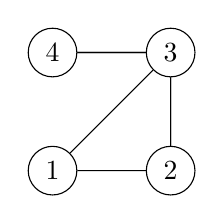
\begin{tikzpicture}[scale=1.5]
  \node[circle,draw] (1) at (0,0) {1};
  \node[circle,draw] (2) at (1,0) {2};
  \node[circle,draw] (3) at (1,1) {3};
  \node[circle,draw] (4) at (0,1) {4};
  \draw (1) -- (2) -- (3) -- (4);
  \draw (1) -- (3);
  \draw (2) -- (3);
  \draw (3) -- (4);
\end{tikzpicture} \]

The adjacency matrix $A$ and degree matrix $D$ for this graph is:
$$A = \begin{bmatrix}0 & 1 & 1 & 0 \\ 1 & 0 & 1 & 0 \\ 1 & 1 & 0 & 1 \\ 0 & 0 & 1 & 0\end{bmatrix} \qquad 
D = \begin{bmatrix}2 & 0 & 0 & 0 \\ 0 & 2 & 0 & 0 \\ 0 & 0 & 3 & 0 \\ 0 & 0 & 0 & 1\end{bmatrix}$$

The Laplacian matrix $L$ is:

$$L = D - A = \begin{bmatrix}2 & 0 & 0 & 0 \\ 0 & 2 & 0 & 0 \\ 0 & 0 & 3 & 0 \\ 0 & 0 & 0 & 1\end{bmatrix} - \begin{bmatrix}0 & 1 & 1 & 0 \\ 1 & 0 & 1 & 0 \\ 1 & 1 & 0 & 1 \\ 0 & 0 & 1 & 0\end{bmatrix} = \begin{bmatrix}2 & -1 & -1 & 0 \\ -1 & 2 & -1 & 0 \\ -1 & -1 & 3 & -1 \\ 0 & 0 & -1 & 1\end{bmatrix}$$

The Laplacian of the graph encodes important information about the connectivity and structure of the graph. For example, the number of connected components of the graph is equal to the number of eigenvectors of the Laplacian with eigenvalue 0. The Laplacian also plays an important role in spectral graph theory, where it is used to analyze the spectral properties of graphs and to design graph clustering algorithms.

\section{Networks for benchmarking}

1. Zachary's karate club network: This is a social network of a karate club that was studied by Zachary in 1977. The network consists of 34 nodes representing members of the club and 78 edges representing friendships between members. It is often used as a benchmark for community detection algorithms.

2. Erdős-Rényi random network: This is a random graph model proposed by Erdős and Rényi in 1959. In this model, a graph is generated by connecting nodes with a certain probability p. Erdős-Rényi random networks are often used as a benchmark for studying properties of random graphs.

3. Barabási-Albert preferential attachment network: This is a random graph model proposed by Barabási and Albert in 1999. In this model, a graph is generated by starting with a small number of nodes and adding new nodes one at a time, with each new node preferentially attaching to existing nodes with higher degree. Barabási-Albert networks are often used as a benchmark for studying properties of scale-free networks.

4. Les Miserables co-occurrence network: This is a network of co-occurrences of characters in the novel Les Miserables by Victor Hugo. The network consists of 77 nodes representing characters and 254 edges representing co-occurrences in the same chapter. It is often used as a benchmark for community detection algorithms.

5. Power grid network: This is a network of the power grid in the western United States. The network consists of 4,941 nodes representing power stations and 6,594 edges representing power lines. It is often used as a benchmark for studying properties of real-world networks.

6. The Southern Women graph is a social network graph that represents the social interactions between women in a Southern US social club in the 1930s. The graph is an undirected graph with 32 nodes (women) and 89 edges (social interactions).

Each node in the graph represents a woman, and an edge between two nodes indicates that the corresponding women interacted socially at the club. The weight of each edge represents the number of social events at which the two women interacted.

\subsection{Random graphs}

Random graphs are mathematical models that are used to study the properties of graphs that arise from random processes. In a random graph, edges are created between nodes according to some probabilistic model, rather than being determined by some underlying structure or pattern.


Example. There are two possible regular graphs with 4 nodes and degree 2: the cycle graph $C_4$
\begin{center}
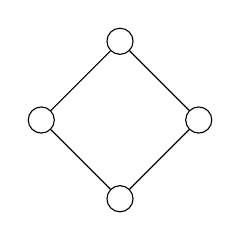
\begin{tikzpicture}
  \node[circle, draw] (A) at (0,0) {};
  \node[circle, draw] (B) at (1,1) {};
  \node[circle, draw] (C) at (2,0) {};
  \node[circle, draw] (D) at (1,-1) {};
  \draw (A) -- (B) -- (C) -- (D) -- (A);
\end{tikzpicture}
\end{center}
 and the disjoint union of two edges $K_2 \cup K_2$ :
\begin{center}
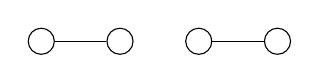
\begin{tikzpicture}
  \node[circle, draw] (A) at (0,0) {};
  \node[circle, draw] (B) at (1,0) {};
  \node[circle, draw] (C) at (2,0) {};
  \node[circle, draw] (D) at (3,0) {};
  \draw (A) -- (B);
  \draw (C) -- (D);
\end{tikzpicture}
\end{center}
These are the only two possible regular graphs with 4 nodes and degree 2, as any other arrangement would either have nodes of degree greater than 2 or have disconnected nodes. An algorithm that randomly produces one of these two graphs, produces random regular graphs.

There are many different models of random graphs, each with their own set of assumptions and properties. Some common models include:
\begin{itemize}
\item Erdős-Rényi model: A model where each edge is present with a fixed probability, independently of all other edges.
\item Watts-Strogatz model: A model where edges are rewired with a small probability, resulting in a graph with a high clustering coefficient but a short average path length.
\item Barabási-Albert model: A model where new nodes are added to the graph one at a time, and each new node is connected to existing nodes with a probability proportional to their degree.
\end{itemize}

\subsection{Random regular graphs}

Random regular graphs are graphs where each vertex has the same degree. The algorithm to generate a random regular graph with $n$ vertices and degree $k$ is as follows:

1. If $n$ is odd or $k$ is odd and $n$ is even, then no random regular graph exists. Otherwise, set $d = \frac{k}{2}$.
2. Create an empty graph $G$ with $n$ vertices.
3. For each vertex $v$, add an edge between $v$ and the $d$ vertices that appear next to it in a cyclic ordering of the vertices.
4. Shuffle the vertices randomly.
5. For each vertex $v$, rewire each of its $d$ edges to a randomly chosen vertex, subject to the constraints that the resulting graph remains $k$-regular and does not contain self-loops or multiple edges.

The resulting graph is a random $k$-regular graph on $n$ vertices.

\begin{algorithmic}[1]
\Require $n$: number of vertices, $k$: degree of each vertex
\State If $n$ is odd or $k$ is odd and $n$ is even, then no random regular graph exists.
\State Otherwise, set $d = \frac{k}{2}$.
\State Create an empty graph $G$ with $n$ vertices.
\For{$i = 1$ to $n$}
    \For{$j = 1$ to $d$}
        \State Add an edge between vertex $i$ and vertex $(i+j) \mod n$.
    \EndFor
\EndFor
\State Shuffle the vertices randomly.
\For{$i = 1$ to $n$}
    \For{$j = 1$ to $d$}
        \State Choose a random vertex $v$ that is not adjacent to vertex $i$.
        \State Remove the edge between vertex $i$ and some neighbor of $i$ that appears $j$ positions after $i$ in the cyclic ordering of vertices.
        \State Add an edge between vertex $i$ and vertex $v$.
    \EndFor
\EndFor
\State Output the resulting graph $G$.
\end{algorithmic}

\subsection{Erdos-Renyi model}
The Erdős-Rényi (ER) algorithm is a popular method for generating random graphs. Given a set of $n$ nodes and a probability $p$ of any two nodes being connected by an edge, the ER algorithm generates a random graph by considering each possible edge and including it with probability $p$.

The ER algorithm can be implemented as follows:
\begin{enumerate}
\item Start with an empty graph $G$ with $n$ nodes.
\item For each pair of nodes $i$ and $j$ (excluding self-loops), add an edge between them with probability $p$. This can be done by generating a random number $r$ between 0 and 1 for each pair of nodes, and adding an edge if $r \leq p$.
\item Output the resulting graph $G$.
\end{enumerate}

\begin{algorithmic}[1]
\Require $n$: number of nodes, $p$: probability of an edge between any pair of nodes
\State Create an empty graph $G$ with $n$ nodes.
\For{$i = 1$ to $n-1$}
    \For{$j = i+1$ to $n$}
        \State Generate a random number $r$ between 0 and 1.
        \If{$r \leq p$}
            \State Add an edge between nodes $i$ and $j$.
        \EndIf
    \EndFor
\EndFor
\State Output the resulting graph $G$.
\end{algorithmic}

The ER algorithm generates a random graph with an expected number of edges equal to $p \cdot \binom{n}{2}$, which is the number of possible edges in the graph multiplied by the probability of each edge being included. The resulting graph is typically sparse for small values of $p$ and becomes increasingly dense as $p$ approaches 1.

%The ER algorithm is a simple and effective way to generate random graphs with a given size and edge density, and it has been widely used in the study of graph theory and network science.

\subsection{Albert Barabasi graphs}

The Barabási-Albert (BA) algorithm is a popular method for generating scale-free graphs, which are graphs with a degree distribution that follows a power law. The BA algorithm generates a graph by starting with a small number of nodes and adding new nodes one at a time, each with a fixed number of edges attached to existing nodes.

The BA algorithm can be implemented as follows:

1. Start with a small graph $G$ with $m_0$ nodes, where $m_0$ is a parameter of the algorithm.
2. Add a new node $i$ to the graph, and connect it to $m$ existing nodes in the graph, where $m$ is a parameter of the algorithm.
3. The probability that node $i$ connects to node $j$ is proportional to the degree of node $j$ in the graph, i.e., nodes with higher degree are more likely to be connected to.
4. Repeat steps 2-3 until the desired number of nodes is reached.

\begin{algorithmic}[1]
\Require $m_0$: number of initial nodes, $m$: number of edges to attach to each new node, $n$: final number of nodes in the graph
\State Create an empty graph $G$ with $m_0$ nodes.
\State Create a list $L$ of nodes, where each node appears $m_0$ times in the list.
\For{$i = m_0$ to $n-1$}
    \State Create a new node $v_i$.
    \State Choose $m$ distinct nodes to connect $v_i$ to, sampled from $L$ with probability proportional to their degree.
    \State Add edges between $v_i$ and the chosen nodes.
    \State Add $m$ copies of $v_i$ to $L$.
\EndFor
\State Output the resulting graph $G$.
\end{algorithmic}

The resulting graph generated by the BA algorithm has a degree distribution that follows a power law, which means that a few nodes have a very high degree while most nodes have a low degree. This property is characteristic of many real-world networks, and it has important implications for the behavior of these networks.

The BA algorithm is a simple and elegant way to generate scale-free networks, and it has been widely used in the study of network science and related fields.

\section{Practical Python Class: networks}

\subsubsection*{Graph metrics in Les Miserables}



\section{Practical Homework}

\subsubsection*{Graph structure in written Chinese}

Take the list of Chinese words. Define a graph $G$ where each node is one Chinese character. Define a link between two nodes whenever there is at least one word with both characters.
\begin{enumerate}
 \item What is the degree distribution in $G$?
 \item Show examples of the characters with highest and smallest degree.
 \item Make a histogram of degree distribution? Is it heavytailed?
 \item Define the same graph, bot now directed, where direction is defined by the ordering of the characters in the words: $AB \Rightarrow (A\to B)$. Make the histogram of out-degree and in-degreen for the directed graph.
 \item Show examples of the charactes with highest out and in degrees.
 \item Make a hisogram of the out and in degrees.
 \item Define the unbalance, as the difference between out and in-degrees. Make a histogram of the unbalance.
 \item Show examples of characters with the high positive and negative unbalances. Is there a linguistic reason for this?
\end{enumerate}


\section{Percolation an epidemics}




 \chapter{Monte Carlo simulation of epidemics}

So, epidemics are stochastic proceses. Some analytical results exist, for the simpest of cases, as the SIR or SIS dynamics. In more complex cases, simulations are the only tool at hand to study their dynamics.

As we mentioned in last chapter, epidemics can be seen as a set of stochastic reactions, turning healthy people into infectious, and turning them into recovered, at certain rates. Next we discuss how to simulate such types of procceses in a computer.

%  Sources:
%  https://www.normalesup.org/~doulcier/teaching/adaptive_dynamics/dyad02.html
%  https://courses.maths.ox.ac.uk/pluginfile.php/20809/mod_resource/content/2/lec9.pdf
%  

\section{Rates and exponential distributions}

\subsubsection*{Exponential distribution}

As you shall remember (see appendix) from your probabilies class, the exponential distribution is the continuous time limit of a process in which you flip a coin as many times as needed until you find the first ``head'' coming out \footnote{In appendix of this chapter, you will find a brief reminder of what conditional probability means, and the deduction of the continuos exponential distribution as a limit of a Bernoulli process, if you are interested to check.}. It is clear from the nature of this process, that if a head has not shown up after we toss the coin 5 times, then the probability that it will appear in the next $x$ shots, is the same probability that it had in any $x$ shots, regardless of the fact that we already shot it 5 times. This results in a very important property of exponential distributions: they do not have memory.

The probability density of the exponential distribution is
\[ f(x) = {\lambda} e^{- \lambda x}
\]
The cumulative distribution function is therefore
\[ F(x) =  \int_{-\infty}^x  f(x) = 1-e^{- \lambda  x} \] (defined only for $x>0$, with $F(x)=0$ otherwise), and the mean value $\langle X \rangle = \frac 1 \lambda $.


{\bf memorylessness of exponential random variables}

Let's look at an interesting case. Let's prove that the exponential distribution has no memory. This means the following:
\[P(X> s+t | X>s) = P(X>t)
\]
This property is called memorylessness because the probability of $X>s+t$ given that $X>s$ is independent of the value of $s$. Using the definition of conditional probability,
\[P(X> s+t | X>s) = \frac {P(X> s+t, X>s)}{ P(X>s)}  
\]
But $P(X> s+t, X>s) = P(X> s+t ) $, since the set $\{x:x>s+t\} \subset \{x:x>s\}$. Note that here the notation $P(A,B)$ corresponds to the probability of both $A$ and $B$ occurring simultaneously, that is, $P(A\cap B)$. Therefore,
\[P(X> s+t | X>s) = \frac {P(X> s+t)} {P(X>s)}  
\]
The probabilities $P(X>a) = 1 - F(a)$, so $P(X>s+t)  =  e^{-\lambda (s+t)} $ and $P(X>s)  =  e^{- \lambda s}$, from which
\[P(X> s+t | X>s) = \frac {P(X> s+t)}{ P(X>s)}  = \frac {e^{- \lambda(s+t)}} {e^{-\lambda s}}  =  e^{-\lambda  t } = 1-F(t) = P(X>t)\]
thus concluding the proof.

This property of the exponential density has the following physical implication. The decay of a radioactive atom is a process that occurs with exponential probability. The lack of memory of this probability means that regardless of the past lifetime of an atom, its probability of decaying in the future is always a decreasing exponential.

{\bf Law of the minimum of independent exponential variables:}

Another fundamental result for the following discussion is the following propertie of exponential r.v.:
\begin{equation*}
\begin{cases}
X_i \sim \mathcal Exp(\lambda_i), \\
Y_i=\min_i X_i, \\ Z_i = 
\text{argmin}_i X_i 
\end{cases}
\Rightarrow
\begin{cases}
Y \sim \mathcal Exp(\sum_i \lambda_i) \\
\mathbb P(Z=i) = \frac{\lambda_i}{\sum_j \lambda_j}
\end{cases}
\end{equation*}

The proof of which is left to the interested student.


\section{Gillespie's Stochastic Simulation Algorithm}

The Gillespie algorithm is a stochastic simulation algorithm that is often used to simulate chemical reaction systems. It simulates the time evolution of a reaction system by randomly selecting which reaction will occur next and when it will occur.

Consider the following chemical reaction system:
\begin{align}
A + B &\xrightarrow{k_1} C + B\\
C &\xrightarrow{k_2} 2 D  \\
2 D + B&\xrightarrow{k_3} A 
\end{align}
where $A$, $B$, $C$, and $D$ are chemical species, and $k_1$, $k_2$, and $k_3$ are reaction rate constants.

The interpretation of this list of reactions is the following. We have a system with a certain ammount of elements $X=(n_A,n_B,n_C,n_D)$ at time $t$. At any moment in time, any of the three reactions can take place. Let us call $\Delta X_r$ the vector of the effect that reaction $r$ has on the system, in this case:
\[  \Delta X_1= \begin{pmatrix} 
              -1\\
              0 \\
              1\\
              0
             \end{pmatrix}
\qquad  \Delta X_2= \begin{pmatrix} 
              0\\
              0 \\
              -1\\
              2
             \end{pmatrix}
\qquad \Delta X_3= \begin{pmatrix} 
              1\\
              -1 \\
              0\\
              -2
             \end{pmatrix}
\qquad \]

So, the stochastic proccess is actually defined by a sequence of growing times $t_{k-1}< t_{k}$ at which reactions occur, and the index of the reaction occurring:
\[ \mathcal P = \{ (t_1, r_1), (t_2, r_2).. \}\]
such that the stochastic variable is given by 
\[ X(t) = X(t_{k-1}) + \Delta X_{r_k} \]
where $k$ is such that $t_{k-1} <t < t_{k}$. In other words, the $t_k$ are the moments in which reactions occur, and at those points, the state of the system changes from $X(t)$ to $X(t+\ud t) = X(t^+) = X(t) + \Delta X_{r_k}$.

So, simulating such stochastic process amounts to defining a way to generate the stochastic squence $\mathcal P$. Furthermore, this process is a Markov process, meaning that the values of $(t_k, r_k)$ depend only on the current state of the system $X(t_{k-1}^+)$.

\subsection{Gillespie's algorithm}

To simulate this system using Gillespie's algorithm, we first define the propensity functions for each of the three reactions:

\begin{align}
a_1 &= k_1 [A][B] \\
a_2 &= k_2 [C] \\
a_3 &= k_3 [D]^2 [B]
\end{align}
where $[A]$, $[B]$, $[C]$, $[D]$, and $[E]$ are the concentrations of the corresponding chemical species.

We then randomly select the time $\tau$ until the next event occurs and the reaction that will occur next. The probability that reaction $i$ will occur next is given by:
\begin{equation}
P_i = \frac{a_i}{\sum_j a_j}
\end{equation}
where the sum is taken over all reactions.

Once we have determined which reaction will occur next, we update the concentrations of the chemical species according to the stoichiometry of the reaction. This is summarized in the algorithm \ref{alg:gillespie}.
\begin{algorithm}{Gillespie SSA}
\begin{algorithmic}[1]
\State $t = 0$
\State $X(0) = X_0$ \Comment {Set initial state }
\While{$t < t_{end}$}
    \State Update($a_i$) \Comment{Calculate each reactions propensity}
    \State $a_0 = \sum_i a_i$ \Comment{Total propensity}
    \For{$i=1\ldots K$}\Comment{Compute probabilities for every reaction}
    \State $P_i = \frac{a_i}{a_0}$ 
    \EndFor
    \State $r_1 \sim U(0,1) $ \Comment{Generate random numbers, $r_1$ and $r_2$}
    \State $r_2 \sim U(0,1) $    
    \State $\tau = \frac{1}{a_0} \ln\frac{1}{r_1}$ \Comment{Time until the next reaction}
    \State $k = i | \sum_k^{i-1} P_k < r_2 <\sum_k^i P_{i}$ \Comment{Next reaction with probability $P_i$}
    \State $X(t+\tau) = X(t) + \Delta X_k$
    \State Set $t = t + \tau$
\EndWhile
\end{algorithmic}
\label{alg:gillespie}
\caption{}
\end{algorithm}

This example illustrates how Gillespie's algorithm can be used to simulate the time evolution of a simple chemical reaction system. By defining the propensity functions and randomly selecting the next event, we can simulate the stochastic behavior of the system and gain insight into its dynamics.


\section{Practical Python class}

In this practical class we will program the Gillespie algorithm for stochastic simulations in Python. I will share with you a Jupyter Notebook.

Once the algorithm is running, we will test it in three different models:
\begin{enumerate}
 \item Drunken man model
 \item SIR model
 \item SIS model
\end{enumerate}

In the first two cases, we will compare the results of the simulation with the known analytical solution.



\section{Practical Homework}

Consider the model SIRS, as follows:
\begin{eqnarray*}
 S + I &\xrightarrow{\beta}& 2I \\
 I &\xrightarrow{\mu}& R \\
 R &\xrightarrow{\eta}& S \\
\end{eqnarray*}

\begin{enumerate}
 \item Make a simulation of a system of $N=1000$ individuals with parmeters $\beta = 0.02$, and $\mu=\eta=0.01$. Use as initial condition $(n_S,n_I,n_R) = (N/3,N/3,N/3)$.
 \item By visual inspection in your previous simulation, define a value of $T$ where the system is at equilibrium (approximately not changing).
 \item Study the long time behavior of this system for a range of values of $\beta \in (0.001,0.002,0.003,\ldots$ $0.009,0.01,0.011,0.012$ $\ldots,0.02)$
 \item Write down the differential equations for this system.
 \item Study the steady state analytically, by setting all time derivatives to zero, and solving for the other equilibrium values of $S,I$ and $R$.
 \item Compare to the long time study as a function of $\beta$.
\end{enumerate}
 



\section*{Appendix: Conditional probability}
The continuous conditional distribution has the usual expressions $P(A|B) = P(A B)/P(B)$. In the case of continuous random variables, the probability of any event is given by integrating the probability density over the set of points that constitute the event $P(A) = \int_A \ud x f(x)$, so that
\[
P(A|B) = \frac{\int_{A B} \ud x f(x)}{\int_B\ud x f(x)}
\]
The independence of events A and B is equivalent to either of the equalities
\[ P(A B) =P(A) P(B) \qquad P(A|B ) = P(A) \]



\section*{Appendix: Exponential distribution}


As you shall remember from your probabilies class, the exponential distribution is the continuous time limit of a process in which you flip a coin as many times as needed until you find the first ``head'' coming out. What follows is a deduction of such property.

Let's consider the case of waiting time in a Bernoulli process with success probability $q$. Let $K\in \{1,2,3,\ldots\}$ be the corresponding discrete random variable for the number of experiments that must be performed until the first successful result occurs. The distribution of $K$ is given by:
\[ P(K=k) = (1-q)^{k-1} q
\]
To understand the following steps, let's think of $K$ as the number of time intervals we must wait until we observe success. Now, suppose we want to discretize time into smaller intervals, and let's focus on the variable $X = K/N$ where $N$ is the number of intervals in which one second is divided. Let's also consider, as is natural, that the divisions of the intervals do not affect the real probability of the phenomenon, so $q=q'/N$. In this way, the probability density of the variable $X$ is obtained as the limit $N\to \infty$ from the variable $K$, known as the continuous limit:
\begin{eqnarray*}
 P(X = k/N) &=& P(K=k) = (1-q)^{k-1} q \\
	    &=&  (1-\frac{q'}{N})^{N x-1} \frac{q'}{N} \\
f(x) &=& \lim_{N\to\infty} \frac{P(X = k/N)}{1/N}	=  q' e^{-x q'}
\end{eqnarray*}

The resulting distribution is called the exponential density, and is usually expressed in terms of the parameter $\lambda = 1/{q'}$
\[f(x) = \frac{e^{-x/\lambda}}{\lambda}
\]





 \chapter{Mean field solution of epidemics on Networks}


The well-mixed SIS model is represented by these ``reactions''
\begin{eqnarray*}
 S + I &\xrightarrow{\beta}& 2I \\
 I &\xrightarrow{\mu}& S  
\end{eqnarray*}
and the dynamics variables corresponded to the ammount of elements of each specie: $\bm{n} = (n_S,n_I)$. 
In such model there is no consideration for the spatial structure of the epidemic, a factor that is fundamental in reality. A way to introduce space into epidemics is to study contact networks, {\it i.e.} a graph $G(V,E)$ of individuals $i \in \{1,\ldots,N\}$, whose epidemic state is represented by $X_i(t) \in \{S,I,R\}$ or $X_i \in \{S,I\}$ in the SIS model, and whose possible interactions with other individuals is defined by the edges of the graph $(i,j)\in V$.

In what follows we focus on continuous time compartment epidemic models on networks. Now, instead of a global reaction with a global rate, we have a set of reactions for every given node of the graph:
\begin{eqnarray*}
  X_i &\xrightarrow{r_{S}(X_i,X_{\delta i})}& S \\
  X_i &\xrightarrow{r_{I}(X_i,X_{\delta i})}& I
\end{eqnarray*}
The standard susceptible-infectious-susceptible model (SIS) considers the nodes to be in either of two compartments (states):
\begin{itemize}
 \item $X_i = 0 \equiv S \Rightarrow \mbox{susceptible}$
 \item $X_i = 1 \equiv I \Rightarrow \mbox{infectious}$ 
\end{itemize}
and is the simplest standard for recurrent transmissible diseases. The epidemic is thus a continuous time stochastic process with only two admitted transitions occurring at
\begin{itemize}
 \item rate $\beta$, at which a link $(i,j)$ can transmit the state $1$ from node $i$ to $j$;
 \item rate $\mu$ at which state $1$ decays to state $0$ on any infectious node.
\end{itemize}
Explicitly the set of reactions on a single node are
\begin{eqnarray*}
X_i:\quad  S &\xrightarrow{  r(X_{\delta i})}& I \qquad \mbox{with rate } r(X_{\delta i}) = \beta \sum_{j\in \delta i } \delta_{X_j,I} \\
X_i:\quad  I &\xrightarrow{\phantom{xx}\mu\phantom{xx}}& S
\end{eqnarray*}
assuming the simplest case of homegeous links in the network (all with the same $\beta$). The fact that 
\begin{itemize}
 \item transition rates are independent of time
 \item and infection rates are additive
\end{itemize}
are simplifications valid in the exponential case, but could be not valid (and are not) in general. For instance, the time a person is infecious from a given desease, has more a bell shape than an exponential.

These extensive set of reactions, define a transition rate over the entire stochastic system 
$\bm{X} = (X_i,\ldots,X_N)$, susceptible of being treated with the same tools we studied before:
\begin{itemize}
 \item Numerically: Gillespie's Stochastic Simulation Algorithm (SSA) 
 \item Analytically: master equation
\end{itemize}

In this class we are going to study both approaches. An analytical treatment of the master equation will be in general impossible, and some approximations, under the general cathegory of mean field approximations, can be used instead.

\section{Master equation}

Any continuous time dynamic graphical model with binary variables $\sigma \in \{-1,1\}$ (in our case $X \in \{S,I\}$), can be formally described by a master equation.  The dynamics are fully defined by the rate $r_i(\bm{\sigma})$, which is the probability per unit of time that the variables change their states from $s_i \rightarrow -s_i$. The distribution $P(\bm{\sigma},t)$ is the probability that the system is in the state $\bm{\sigma}$ at time $t$, and the configuration space of this stochastic process is governed by the joint master equation:
\begin{equation}
\frac{\ud P ({\bm\sigma}) }{\ud t} = - \sum_{i=1}^N \Big[
r_i({\bm\sigma}) P ({\bm\sigma}) - r_i(F_i({\bm\sigma})) P (F_i(\bm{\sigma}) ) \Big],
\label{eq:originalME}
\end{equation}
where $F_i$ represents the inversion operator on variable $i$, i.e. $F_i (\bm{\sigma}) = {\sigma_1, \dots, -\sigma_{i}, \dots, \sigma_N}$ and we have omitted the time dependence of $P(\bm{\sigma}) = P(\bm{\sigma},t)$ for simplicity of notation. This is a balance equation. The first term inside the summation accounts for transitions from the state $\bm{\sigma}$ of each of the elements of the system, and the second term accounts for transitions from any configuration of the system to the state $\bm{\sigma}$.

This equation is exact, but it is impractical for treating medium-sized systems since it represents a set of $2^N$ (for an $N$-variable system) coupled differential equations. However, in a system of local interactions, where the connections are given by a graph and the transition rates $r_i(\bm{\sigma}, t)$ depend only on the spin configuration $i$ and its neighborhood $\partial_i$, the system can be described by differential equations of the individual probability $P (\sigma_i)$.



Taking into account the topology of the system, a master equation for the probability $P (\sigma_i)$ of each node in the system can be written as:  
\begin{eqnarray}
\frac{\ud P (\sigma_i) }{\ud t} = - \sum_{\sigma_{part i}} \Big[
r_i(\sigma_i, \sigma_{part i}) P(\sigma_i, \sigma_{part i})
-  r_i(-\sigma_i, \sigma_{part i}) 
P(-\sigma_i, \sigma_{part i}) \Big]
\label{eq:CMEPi_pij} 
\end{eqnarray}
where $\partial_i$ is the neighborhood of node $i$ and $P(\sigma_i, \sigma_{part i})$ is the joint probability of a configuration of node $i$ and its neighborhood. This new system of equations is still exact, and the probability $P(\bm{\sigma})$ can be calculated as the product of the individual probabilities $\big[ \prod_{i=0}^N P(\sigma_i)$ of all nodes in the system. But unlike equation (\ref{eq:originalME}), this set is not a closed set of differential equations, because the time evolution of the joint probabilities is not known.


\section{Mean field approximations to the SIS model} \label{sec:MF}

Mean field approximations for deriving continuous-time differential equations for epidemic processes on contact networks are fundamentally based on considering correlations between the expected values of random variables up to a certain level of factorization, usually the first two.



Attempts to reduce the complexity start from factorizing the single master equation into many equations for each node marginals $P_i(X_i,t)$. Given that the $X$'s are two-state variables, $P_i(X_i)$ consists of two values $P_i(X_i = 0)$ and $P_i(X_i = 1)$, where we have identified the susceptible state as $X=0$, and the infectious as $X=1$. Futhermore, since $P_i(X_i=0) = 1 - P(X_i=1)$, only one value is enough to represent $P(X_i)$. In the particular choice of $S\to 0$ and $X \to 1$, it is the case that $P_i(X_i=1) = \E [X_i] $, such that the master equation can be written as an evolution of the expected values of the infectious state: 
\begin{equation}
\frac{\ud \E\left[  X_{i}\left(  t\right)  \right]  }{\ud t}  =\E\left[  -\mu
X_{i}\left(  t\right)  +\beta (1-X_i(t))   
\sum_{j=1}^{N}a_{ij}X_{j}\left(  t\right)  \right]
\label{eq:meanXdt}
\end{equation}
where $a_{ij}$ are the elements of the adjacency matrix, meaning that $a_{ij} = 1$ if nodes $i$ and $j$ are neighbors ($(i,j)\in E$) and is zero otherwise.

However, the expectation value on the right hand side acts over products of variables $X_j(t) (1-X_i(t))$, which requires a differential equation for the evolution of the correlations. Not surprisingly, the two point correlations functions depend on three point correlations and so on and so forth. 


\subsection{Individual-based mean field (IBMF) approximation}


The simplest closure of equation eq.  (\ref{eq:meanXdt}) is the individual-based mean field (IBMF) in which independence is assumed $\E[X_i(t) X_j(t)] \approx \E[ X_i(t)] \: \E [ X_j(t)] \equiv \rho_i(t) \varrho_j(t)$ ($\varrho_{i}$ is the probability that node $i$ is infectious) and therefore eqs. (\ref{eq:meanXdt}) are now a closed set of non linear different ial equations:
\begin{equation}
\frac{d \rho_i(t)  }{dt}=-
 \mu \, \rho_i(t)  +\beta [1-\rho_i(t)] \sum_{j \in \partial i} 
\rho_j(t)
\label{eq:IBMFSISequations}
\end{equation}
where we used the notation $\partial i$ to represent the set of neighbors of node $i$.

\subsection{Pair-based mean field (PBMF)}

The second simplest way to close the equations is to consider a differential equation for the correlations between neighboring variables $X_i X_j$. We, therefore, need a master equation for the evolution of such products. Such equation is given by
\[ \frac{\ud \E X_i X_j}{\ud t} = \E \left[ -2\mu X_i X_j +\beta X_j (1-X_i )\sum_{k=1}^N a_{ik} X_k + \beta X_i (1-X_j )\sum_{k=1}^N a_{jk} X_k  \right]  
\]
A reordering of the terms results in 
\begin{eqnarray}
\frac{\ud \E\left[  X_{i}X_{j}\right]  }{dt}  
&  =& -2\mu \E[X_{i}X_{j}] + \beta\sum_{k=1}^{N} a_{ik}\E[X_{j}X_{k}] + \beta\sum_{k=1}^{N} a_{jk}\E[X_{i}X_{k}]  \nonumber \\
&& \phantom{-2\mu \E[X_{i}X_{j}]} -\beta\sum_{k=1}^{N}(a_{jk} +a_{ik}) \E[X_{i}X_{j}X_{k}]
\label{eq:EXiXidt} 
\end{eqnarray}
but a factorization is assumed for higher correlations. Different approaches have been used to approximate $\E[X_i X_j X_k]$ in terms of smaller correlations. In this paper we will compare with the approximations proposed in \cite{cator2012second} $\E[X_i X_j X_k] \approx \E[X_i X_j]\E[X_k] \equiv \phi_{ij}(t) \, \rho_i(t)$:
%\begin{eqnarray}
% \frac{\ud\rho_{i}(t)}{\ud t} &=& -\mu \rho_{i}(t) + \beta \sum_{j \in \partial i} \left[ %\rho_{j}(t) - \rho_{ij}(t) \right] \label{eq:rhoi_dt_PBMF} \\
% \frac{\ud \rho_{ij}(t)}{\ud t} &=& -2 \mu \rho_{ij}(t) + \beta \left[ \rho_{i}(t) + %%\rho_{j}(t) - 2 \rho_{ij}(t) \right] + \nonumber \\
% & & + \; \beta \sum_{k \in \partial i \setminus j} \left[ \rho_{jk}(t) - \rho_{ij}(t) \rho_{k}(t) \right] + \beta \sum_{k \in \partial j \setminus i} \left[ \rho_{ik}(t) - \rho_{ij}(t) \rho_{k}(t) \right] \label{eq:rhoij_dt_PBMF}
%\end{eqnarray}
\begin{eqnarray}
 \frac{\ud\rho_{i}(t)}{\ud t} &=& -\mu \rho_{i}(t) + \beta \sum_{j \in \partial i} \phi_{ij}(t)  \label{eq:rhoi_dt_PBMF} \\
\frac{\ud \phi_{ij}(t)}{\ud t} &=& -(2\mu+\beta) \phi_{ij}(t) + \mu \rho_i(t)-  \beta \phi_{ij}(t) \sum_{k \in \partial j \setminus i} \rho_{k}(t)  \nonumber \\ & & + 
\beta \left[ 1 - \rho_{i}(t) - \phi_{ij}(t) \right] \sum_{k \in \partial i \setminus j} \rho_{k}(t) \label{eq:joint_PBMF1}
\end{eqnarray}
and \cite{mata2013pair} $\E[X_i X_j X_k] \approx \frac{\E[X_i X_j]\E[X_j,X_k]}{E[X_j]} \equiv \frac{\phi_{ij}(t) \, \phi_{kj}(t)}{\rho_{j}(t)}$.
\begin{eqnarray}
 \frac{\ud\rho_{i}(t)}{\ud t} &=& -\mu \rho_{i}(t) + \beta \sum_{j \in \partial i} \phi_{ji}(t)  \nonumber \\
\frac{\ud \phi_{ij}(t)}{\ud t} &=& -(2\mu+\beta) \phi_{ij}(t) + \mu \rho_i(t)  -  \beta \phi_{ij}(t)/(1-\rho_{j}(t)) \sum_{k \in \partial j \setminus i} \phi_{kj}(t)  \nonumber \\ & & + 
\beta \left[ 1 - \rho_{j}(t) - \phi_{ij}(t) \right]/(1-\rho_{i}(t)) \sum_{k \in \partial i \setminus j} \phi_{ki}(t)
\label{eq:joint_PBMF2}
\end{eqnarray}

We will refer to the two different approximations shown in (\ref{eq:joint_PBMF1}) and (\ref{eq:joint_PBMF2}) as {\bf PBMF-1} and {\bf PBMF-2}, respectively. 

In both approaches, IBMF and PBMF, the expected values evolving in time are intended to be expectations over different stochastic stories of the whole epidemic process. Therefore they are to be compared with averages over many Monte Carlo simulations of such process.

% \section{Endemic (steady) state }
% We analytically compute the epidemic size in the endemic state for these approximations for random regular graphs. Since every node has the same degree $k$, the equations are similar for every node, and we can assume that in the steady state the topology is averaged out, and all the probabilities are the same, regardless the node indexes.
% 
% Working explicitly for the CME approximation, stationarity means we have to set $\frac{\ud p_i }{\ud t}$ and $\frac{\ud \pij }{\ud t}$ to $0$ in equations (\ref{eq:CMESISpi}) and (\ref{eq:CMESISpij}):
% \begin{eqnarray}
%   \mu p_i &=&  \beta (1-p_i)\sum_{k} p_{ki} \equiv \beta (1-p_i) k \pij \\
%    \mu \pij &=& (1-\pij) \beta \sum_{k \in part i \setminus j}  p_{ki} \equiv (1-\pij) \beta (k-1)
% \end{eqnarray}
% % 
% % As the graph is a random regular and each node has $k$ neighbors in the stationary state each $p_i$ and $\pij$ should has the same value so:
% % \begin{eqnarray}
% %   \mu p_i &=&  \beta (1-p_i) k \pij \\
% %   \mu \pij &=&  (1-\pij) \beta (k-1) \pij 
% % \end{eqnarray}
% where now the indices $i$ and $i,j$ are generic. Solving this system of equations we get for the two variables $p_i$ and $p_{ij}$:
% \begin{eqnarray}
%  p_i &=&\frac{\lambda(k-1)-1}{\lambda(k-1)-1+(k-1)/k} 
%   %\frac{1}{1+\frac{\mu}{k\beta(1-\frac{\mu}{(k-1)\beta})}} 
%   \qquad   \pij =  1- \frac{\mu}{(k-1)\beta}  
% \end{eqnarray}
% This can be already tested against simulations of random regular graphs. Furthermore we can obtain the spreading rate or effective infection rate $\lambda = \beta/\mu$ above which there is an endemic outbreak (sustained in time epidemic) by solving $p_i(k) = 0$, resulting in the epidemic threshold $\lambda_c = 1/(k-1)$. A similar procedure for all five approximations results in table \ref{tb:table_endemic_state}. 
% 
% The critical values $\lambda_c=1/k$ for IBMF are consistent with those in  \cite{pastor2015epidemic} and citations therein with similar approaches. PBMF-2 prediction $\lambda_c = 1/(k-1)$, however, is known to be a second order correction to the endemic threshold \cite{mata2013pair,cator2012second}, and it is numerically \cite{mata2013pair,ferreira2012numeric} seen to outdo the individual based value.
% 
% 
% 
% %(y+y*(y-1)*x-2/x-1)/((y-1)*(x*y+2))
% \begin{center}
% \begin{table}
% \def\arraystretch{2.5}
% \begin{tabular}{|c|c|c|}
%  \hline Approximation & Endemic state (equilibrium) & $\lambda_c$ \\
% \hline
% %& & \\
%  IBMF & \(p_i =  1 - \frac{1}{k\lambda} \) & $\lambda_c = \frac{1}{k}$\\
% %& & \\
% \hline
% %& & \\
%  PBMF-1 & $p_i = \frac{k+k(k-1)\lambda-2/\lambda -1}{(k-1)(\lambda k +2)}$ & $ \lambda_c = \frac{\sqrt{1+\frac{8k}{k-1}}-1}{2 k} $\\
% %& & \\
% \hline
% %& & \\
%  PBMF-2 & $p_i = \frac{\lambda(k-1)-1}{\lambda(k-1)-1+(k-1)/k}$ & $ \lambda_c = \frac{1}{k-1} $\\
% %& & \\
% % \hline
% % %& & \\
% %  rDMP & $\begin{array}{lcl}  
% %  p_i &=&  1- \frac{1}{(k-1)\lambda} \\
% %   \pij &=&   \frac{(k-1) \lambda-1}{k \lambda} 
% % \end{array}$
% %  &  $\lambda_c = \frac 1 {k-1}$\\
% % %& & \\
% % \hline
% % %& & \\
% %  CME & $\begin{array}{lcl}
% % p_i &=&\frac{\lambda(k-1)-1}{\lambda(k-1)-1+(k-1)/k}  \\
% %   \pij &=&  1- \frac{1}{(k-1)\lambda}  
% % \end{array}$
% %  & $\lambda_c = \frac 1 {k-1}$ \\ 
% %  %& & \\ 
%  \hline
% \end{tabular}
%  \caption{Steady state and epidemic threshold $\lambda_c$ under four approximations: IBMF, PBMF}%, rDMP and CME}
%  \label{tb:table_endemic_state}
%  \end{table}
% \end{center}
% 
% 
% In figure \ref{fig:Eq_vs_R0} we present the analytical predictions of each approximation for the epidemic size $p_i$ at the steady state as a function of $\lambda$. When compared to Monte Carlo results, mean field approximations (IBMF and PBMF-1) give an overestimation of the epidemic size at small $\lambda$, and rDMP an underestimation at large $\lambda$. Meanwhile, CME and PBMF-2 seems to be a better prediction mixing the large $\lambda$ behavior of IBMF and PBMF-1 with the small $\lambda$ behavior of rDMP.
% 
% The results presented in figure \ref{fig:Eq_vs_R0} are very similar to those shown in \cite{gleeson2013binary} where a tractable master equation is presented for the evolution in time of the epidemic size in a graph with the same degree. This description has more resemblance with a degree base aproximation and, as in our case, it catches with similar accuracy the value of the epidemic threshold for a random regular graph of conectivity 3.
% 
% \section{Average case : THIS IS NOT READY, DONT READ}
% \label{sec:average}
% The systems of equations defining IBMF, PBMF, rDMP and CME could be large and delicate to solve on a given graph, although a simple numerical integration normally works. However, in many cases we are interested in general predictions for certain families of graphs or topologies. In this section we derive an average version of the CME approximation to characterize SIS epidemics on uncorrelated random graphs. Our approach relates closely to that in \cite{goltsev2012localization, van2012epidemic}, based on IBMF approximation, where the prevalence at the stationary state is derived just above the epidemic threshold. %In our case based on averaging CME we are presenting a master equation to the prevalence.    
% 
% 
% \begin{figure}
%  \includegraphics[width=0.43\textwidth]{Steady.eps}
%   \includegraphics[width=0.43\textwidth]{epidemic_treshold.eps}\caption{ {\bf Left}: Comparison between Monte Carlo simulations and the predicted endemic equilibrium for each approximation as a function of $\lambda$ for random regular graphs. Each MC point is an average of the last value of of the probability of infected computed for $10^4$ simulations over the 1000 nodes in the system. {\bf Rigth}: Comparison between the epidemic threshold predicted by the methods as a function of graphs connectivity. \label{fig:Eq_vs_R0}}
% \end{figure}
% 
% The simplest description of a graph ensemble is given by the distribution of degrees of its nodes. In the case of uncorrelated graphs, that distribution is the full description of the ensemble. One of the firts theoretical approaches used for epidemic modeling on  networks was the degree based mean field approach (DBMF) \cite{pastor2001epidemic}. It provided a set of master equations for the probability of a node of degree $k$ to be infected at time $t$, assuming statistical equivalence of all nodes of degree $k$. As stated in \cite{pastor2015epidemic} DBMF can be obtained by performing a degree-wise average over the IBMF equations. 
% 
% A similar procedure can be performed in the context of CME. Since the CME equations depend on the information coming from the neighbors in the network, it is expected that nodes more connected will have a different behavior than those less connected. We therefore attempt to reduce the number of equations in our system by characterizing all nodes with the same degree by a couple of average parameters 
% \begin{equation}
%  p^{\gamma}= \frac 1 {N^{\gamma}} \sum_{i:d_i=\gamma+1} p_i \qquad p_{\rightarrow}^{\gamma} = \frac 1 {M^\gamma} \sum_{i:d_i=\gamma+1} \sum_{j \in \partial i} p_{ij}^{\gamma} 
%  \end{equation}
% In both cases the normalization factors count the number of terms in the sums: $N^\gamma$ is the number of nodes with degree  $k = \gamma+1$ while $M^\gamma$ is the number of graph's edges that contain one of these $N^\gamma$ nodes. 
% 
% Averaging the equations (\ref{eq:CMESISpi}) and (\ref{eq:CMESISpij}), and after some simplifications, we get the average CME:
% \begin{eqnarray}
% \dot{p}^{\gamma}&=& -\mu p^{\gamma} + \beta (\gamma+1) (1-p^{\gamma}) \sum_{\gamma^{\prime}} g(\gamma^{\prime}) p_{\rightarrow}^{\gamma^{\prime}}\label{eq:average_pigamma} \\
% \dot{p}_{\rightarrow}^{\gamma}&=& -\mu p_{\rightarrow}^{\gamma} + \beta \gamma (1-p_{\rightarrow}^{\gamma}) \sum_{\gamma^{\prime}} g (\gamma^{\prime}) p_{\rightarrow}^{\gamma^{\prime}} \label{eq:average_pijgamma}
% \end{eqnarray}
% where $g(\gamma)$ is a contact degree distribution. A node extracted randomly from the set of nodes $V$ has degree $k$ with distribution $k\sim P(k)$. However, in order to average the CME equations we rather need to know the excess-degree distribution $g(\gamma)$ of nodes that are sampled by randomly picking up an edge $(i,j)\in E$. Both distributions are related, assuming there is no further correlation in the graph, by:
%  \begin{equation}
%   g(\gamma)=\frac{(\gamma+1)P(\gamma+1)}{\sum_{\gamma}(\gamma+1)P(\gamma+1)} \quad \gamma\in[0,1\ldots].\label{eq:uncorrelated}
%  \end{equation}
% 
%   \begin{figure}
%  \includegraphics[width=0.7\textwidth]{ave_reg_1.eps}
%   \caption{Average probablility of being infected as function of time. The epidemic outbreak was in 10 nodes of each graph of 1000 nodes in in an ensemble of 10 random regular graphs of connectivity 3. Each point of MC is an average over $10^4$ simulations.\label{fig:average}}
% %\caption{Epidemic size as function of time. The epidemic outbreak was in 10 nodes of the graph of 100 nodes and connectivity 3 for each node, with $\beta=0.1$ and $\gamma=0.05$. \label{fig:average_10}}
% \end{figure}
% 
% Following \cite{pastor107066optimal, pastor2001epidemic} we can obtain the endemic threshold in terms of $\Theta = \sum_\gamma g(\gamma) p_{\rightarrow}^{\gamma}$. In the stationary state $\dot{p}^{\gamma} = 0$ and $\dot{p}_{\rightarrow}^{\gamma} = 0$ in (\ref{eq:average_pigamma}) and (\ref{eq:average_pijgamma}) leads to equations for $p^{\gamma}$ and  $p_{\rightarrow}^{\gamma}$ as a function of $\Theta$:
% \begin{equation}
% p^{\gamma}= \frac{\lambda (\gamma+1) \Theta}{1+\lambda (\gamma+1) \Theta } \qquad p_{\rightarrow}^{\gamma}= \frac{\lambda \gamma  \Theta}{1+\lambda \gamma \Theta } . \label{eq:pijtheta} 
% \end{equation}
% Plugging the last equation into the definition of $\Theta$, we obtain a self-consistency equation similar to the one in \cite{pastor107066optimal, pastor2001epidemic, pastor2001epidemic63}
% \begin{equation}
%  \Theta = f(\Theta) \equiv \sum_{\gamma} \frac{(\gamma+1)P(\gamma+1)}{\langle k \rangle } \frac{\lambda \gamma \Theta}{1+\lambda \gamma \Theta }  \label{eq:self-Theta}
% \end{equation}
% which always has a disease-free solution $\Theta = 0$. This solution becomes unstable (endemic case) when  $\partial_\Theta f(\Theta) |_0=1$, which defines the critical parameters resulting in
% \begin{equation}
% \lambda_c = \frac{\langle k\rangle}{\langle k^2\rangle- \langle k\rangle}    \label{eq:non-zero}
% \end{equation}
% where $\langle k \rangle $ is the average node degree. This result improves over the naive mean field prediction $\lambda)c = \langle k\rangle/\langle k^2\rangle$ \cite{pastor2015epidemic}. It trivially contains the result shown in table \ref{tb:table_endemic_state} for CME in random regular graphs and reduces to  it as $\langle k^2 \rangle = \langle k \rangle ^2$. For graphs with Poisson degree distribution (like Erdos-Renyi) $\langle k^2 \rangle = \langle k \rangle ^2 + \langle k \rangle$ the epidemic threshold becomes $ \lambda_c = \frac{1 }{\langle k\rangle}$.



\section{Practical Python Class: simulating epidemics on networks}


{\bf Preclass:} Install Epidemic on Networks (EoN) library on Python

\begin{enumerate}
 \item Simulate an SIR model on the Zachary club graph. Plot the results of $S(t)$, $I(t)$ and $R(t)$.
\item Make an animation of the process.
\end{enumerate}

\newpage
\subsubsection{Homework}
For this homework,  do not code the epidemic process nor the numerical integration of IBMF and PBMF, yourself. 
Please base your code on the EoN library in python.

{\bf Task 1: } Topologies and epidemic threshold for SIS.

As said in the conference, the SIS model corresponds to these reactions
\begin{eqnarray*}
 S + I &\xrightarrow{\beta}& 2I \\
 I &\xrightarrow{\mu}& S  
\end{eqnarray*}
We will study SIS on networks, for different values of the infectivity parameter $\beta$, and for fixed $\mu = 1.0$. It is known that for high values of $\beta$, the epidemic is sustained in time (call endemic), while for low values, the epidemic disapear. The critical value $\beta_c$ is the smallest value tha allows for a sustained epidemic, also known as endemic threshold.

\begin{enumerate}
 \item Study an SIS epidemic for different values of R0 in two topologies: Erdos-Renyi and scale free networks.
\begin{itemize}
 \item Create two large networks ($N=1000$) with the same average degree $\langle k \rangle = 6$, one with an Erdos-Renyi topology, and one with a scale free topology. For the latter, usa an arbitrary exponent $\gamma$ for the distribution, but 
 adjust the parameters to have the same expected degree $\langle k \rangle = 6$.
 \item Show a histogram of the degree distribution in both networks. Compute the expected values $\langle k \rangle$ and $\langle k^2 \rangle$ for both networks.
 \item Use the EoN package in python to simulate epidemics on each of these networks, with starting conditions $I(0)=200$ and $S(0)=800$, randomly selected among the nodes of the network.
 \item Use the EoN package in python to compute the IBMF and PBMF numerical integration of the SIS epidemic on these networks. 
 \item As an example, show the evolution in time of infected individuals for some $\beta$, in both networks, using all threea approaches, the simulation, the IBMF and PBMF approximations.

\item Program a function that, for a given value of $\beta$, computes the average number of infected individuals over many simulations (say 100 simulations). DO NOT USE IBMF/ PBMF, only simulations.

\item Plot the average number of infected individuals at the end of simulations, for different values of $\beta$, for both types of neworks.

\item According to computations discussed in the lecture, the critical value should be related to the degree distribution of the network as 
\[\lambda_c \equiv \frac{\beta_c }{ \mu} = \frac{\langle k \rangle}{\langle k^2 \rangle }.\]
Compare this prediction to the numerical results obtained.

\item Do both topologies have the same epidemic threshold. Why? 
\end{itemize}
\end{enumerate}

\newpage

\begin{enumerate}
 \item Write down the Individual Based Mean Field equations for the SIR model on a network.
 \item Consider SIS model on the Zachary Club graph, starting the epidemic from node 0.
 \begin{itemize}
  \item Compute the average over many simulations of an epidemic.
 \item Compare this average with the results of integrating IBMF and PBMF.
\item What is the average time of infection of node 19 in the simulations?
\item How does it compares with the moment in which probability of infection is 0.5, accroding to both approximations?
 \end{itemize}
\end{enumerate}
 




\subsubsection{Research homework}
Study an SIS epidemic model on the Les Miserables network.
\begin{enumerate}
 \item Run many simulations for different R0 values. Find approximately the epidemic threshold.
 \item Study the epidemic slightly above the epidemic threshold.
 \item Compute the fraction of time that each character is infected, in a long run.
 \item What is the correlation of this time with: clustering coefficient, eccentricity, betweenness of each node?
 \item What is the correlation of this time with the ammount of times that each character is mentioned in the novel?
\end{enumerate}


 
\chapter{Reconstruction of epidemics}

Inference is something you already do. You already know, you are an expert. Except that you only do it intuitively.

{\bf Example 1} If I ask you the age of a person you have zero information about, well you might say it shall be anything between 0 and 120 years old. If I tell you is a friend of mine, well, you probably think that is more probable that his/her age is closer to mine. If I show you a picture, and the person has some gray hair, you move your probability distribution to the higher end of the range, say $50-70$.

{\bf Example 2} If I ask you about the monthly income of a person, you migth say that is something between $0$ and $100$ millions USD a month. If I then tell you that this person graduated from engineering, well, most probably he earns more than $500$ USD a month. If I tell you that he lives in a third world country, chances are higher for a salary below $2000$ USD. If I tell you that lives in India, and that all his friends are rich, that probably raises your salary expectation for this person.

{\bf Example 3} If a little kid (still not talking) comes with fever and crying, there is a lot bunch of diseases that might be the cause. If the mother tells you that in his kindergarten
some kids have been suffering from stomach diseases, well, you can not be sure, but chances are higher for this to be the case.

In all these cases, there is a prior probability distribuion, the one you have in advance of any new information coming to you (that humans live between 0 and 120 years old, most of the time). In all of these cases, that probability distribution changes after you receive new information. You are doing inference.

Mathematically, inference is the procedure by which you update probabilities of certain stochastic variables when you get incomplete information about them. To treat this mathematically, all you need to do is Bayes theorem
\begin{equation}
 P(A|B)\quad = \quad \displaystyle \frac{P(B|A) \quad P(A)}{P(B)} \qquad
 \tikz[baseline=(posterior.base)]{\node[draw, rectangle] (posterior) {Posterior};} =  \frac{\tikz[baseline=(likelihood2.base)]{\node[draw, rectangle] (likelihood2) {Likelihood};} \cdot \tikz[baseline=(prior2.base)]{\node[draw, rectangle] (prior2) {Prior};}}{\tikz[baseline=(evidence.base)]{\node[draw, rectangle] (evidence) {Evidence};}}
\end{equation}
Terms in the Bayes formula have their own names. $P(A)$ is the {\it a priori} distribution, that is, what you know prior to any new information, while $P(A|B)$ --also a probability of event $A$-- is the posterior distribution, what you know {\it a posteriori } that event $B$ --named the evidence-- took place. The term $P(B|A)$ is called likelihood, and $P(B)$ is the probability of the evidence, or just evidence for short.


\section{Inference in graphical models}

The algorithm we care about today has been derived in many different context, many times. It goes by the name of Sum-Product algorithm, or by the name of Belief-Propagation. It is an algorithm for inference in graphical models.

A graphical model is a type of probabilistic model that represents the dependencies between variables using a graph structure. The variables are represented as nodes in the graph, and the relationships between them are represented as edges. For instance a probabilistic model among 6 variables $x_1\ldots,x_6$ given by the interaction functions $\psi_1,\psi_2,\psi_3,\psi_4$ as
\[ P(x_1\ldots,x_6) \propto  \psi_1(x_1, x_2) \psi_2(x_3, x_4) \psi_3(x_4, x_2) \psi_4(x_2, x_5,x_6) \psi_5(x_4)\]

\[
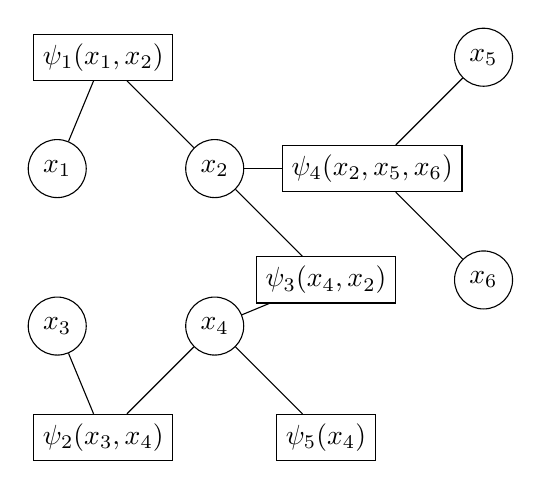
\begin{tikzpicture}[node distance=2cm]
  \node[draw, circle] (x1) {$x_1$};
  \node[draw, circle, right of=x1] (x2) {$x_2$};
  \node[draw, rectangle, right of=x2] (f4) {$\psi_4(x_2, x_5,x_6)$};
  \node[draw, circle, above right of=f4] (x5) {$x_5$};
  \node[draw, circle, below right of=f4] (x6) {$x_6$};
  \node[draw, circle, below of=x1] (x3) {$x_3$};
  \node[draw, circle, below of=x2] (x4) {$x_4$};
  \node[draw, rectangle, above left of=x2] (f1) {$\psi_1(x_1, x_2)$};
  \node[draw, rectangle, below left of=x4] (f2) {$\psi_2(x_3, x_4)$};
  \node[draw, rectangle, below right of=x4 ] (f5) {$\psi_5( x_4)$};
  \node[draw, rectangle, below right of=x2] (f3) {$\psi_3(x_4, x_2)$};
  \draw[-] (x1) -- (f1);
  \draw[-] (x2) -- (f1);
  \draw[-] (x3) -- (f2);
  \draw[-] (x4) -- (f2);
  \draw[-] (x4) -- (f3);
  \draw[-] (x2) -- (f3);
  \draw[-] (x2) -- (f4);
  \draw[-] (x4) -- (f5);
  \draw[-] (x5) -- (f4);
  \draw[-] (x6) -- (f4);
\end{tikzpicture}\]
In this example, we have six variable nodes, $x_1, x_2, x_3,x_4,x_5$ and $x_6$, and four five nodes, given by the functions $\psi_a$. The variable nodes represent the random variables in the model, and the factor nodes represent the factors that depend on these variables. The edges indicate the dependencies between the nodes. This is necessarily a bipartiate graph/.

\example{ {\bf Graph coloring}

Say that every variable takes on three different colors $x_i \in \{white,red,black\} \equiv \{0,1,2\}$. A valid coloring of a graph is such that interacting variables do not have the same color, as in this case
\[
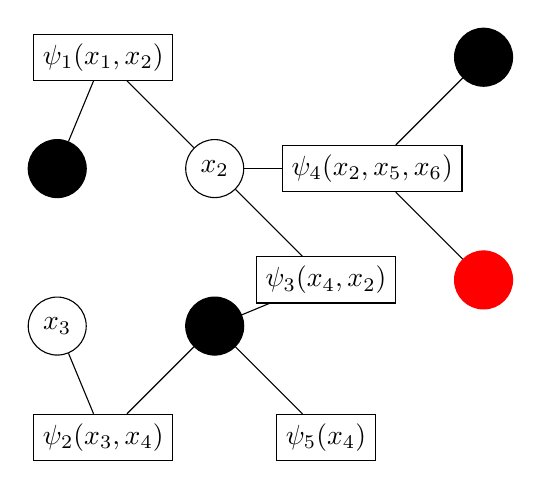
\begin{tikzpicture}[node distance=2cm]
  \node[draw, circle, fill, black] (x1) {$x_1$};
  \node[draw, circle, right of=x1] (x2) {$x_2$};
  \node[draw, rectangle, right of=x2 ] (f4) {$\psi_4(x_2, x_5,x_6)$};
  \node[draw, circle, above right of=f4, fill, black] (x5) {$x_5$};
  \node[draw, circle, below right of=f4, fill, red] (x6) {$x_6$};
  \node[draw, circle, below of=x1] (x3) {$x_3$};
  \node[draw, circle, below of=x2, fill, black] (x4) {$x_4$};
  \node[draw, rectangle, above left of=x2] (f1) {$\psi_1(x_1, x_2)$};
  \node[draw, rectangle, below left of=x4] (f2) {$\psi_2(x_3, x_4)$};
  \node[draw, rectangle, below right of=x4 ] (f5) {$\psi_5( x_4)$};
  \node[draw, rectangle, below right of=x2] (f3) {$\psi_3(x_4, x_2)$};
  \draw[-] (x1) -- (f1);
  \draw[-] (x2) -- (f1);
  \draw[-] (x3) -- (f2);
  \draw[-] (x4) -- (f2);
  \draw[-] (x4) -- (f3);
  \draw[-] (x2) -- (f3);
  \draw[-] (x2) -- (f4);
  \draw[-] (x4) -- (f5);
  \draw[-] (x5) -- (f4);
  \draw[-] (x6) -- (f4);
\end{tikzpicture}\]

How do you define a probabilistic measure that concentrates on top of valid colorings? Well, just define
\begin{eqnarray*}
\psi_{1,2,3}(x,y) &=& (1-\delta_{x,y}) \\
\psi_{4}(x,y,z) &=& (1-(1- (1-\delta_{x,y})(1-\delta_{y,z})(1-\delta_{x,z}))) \\
\psi_5(x) = 1
\end{eqnarray*}
and $P(x_1\ldots,x_6)$ will be zero in all non valid colorings, and will be $1/C$ in all $C$ valid colorings.

 Notice, {\it en passant}, that if you could compute $P(x_1,\ldots,x_6)$ you could inmediately know how many colorings there are, by just inverting any non zero value of $P(\ldots) =1 /C$.

}

The relevance of graphical model is that often they are easy to write down, meaning, it is easy to propose a meaningful set of local interactions that define your particular problem. However, the full probability disitribution is of little use, for the following reasons:
\begin{enumerate}
 \item Most of the time, you want general properities (macro states), not a microscopic description of the system
 \item Evaluation of $P(\ux)$ requieres a normalization constant, and that needs a trace over all configurations of the system, which typically is exponetially many
 \item Sometimes you care about specific variables $P_i(x_i) = \sum_{\ux \setminus x_i} P(\ux)$, that also requires an unfeasible sum.
\end{enumerate}
The first issue relates to the definition of observables in statistical mechanics, while the second relates to the partition function. The third issue is less typical of statistical mechanics, but yet, connected to the approximations we typically use to solve the first two.

%Note that the rectangular nodes represent the factor nodes, while the circular nodes represent the variable nodes.

\subsection{Supersonic intro to statistical mechanics}

In statistical mechanics, the partition function and the free energy are important quantities that describe the thermodynamic properties of a system. How does that has anything to do with inference? Well, maybe it will be clearer later, but for the time being let us say that thermodynamic porperties equals general macroscopic properties of a system, and statistical mechanics make the connection between those general properties and the details of the interactions in the system.

Consider, for instance, a graphical model as the previous one. Since the overall probability of the system is given by a product of functions, it is convenient (more on this later) to write each function as an exponential:
\[ \psi_a(\ux^a) = e^{ -\beta E_a(\ux^a) }\]
where $\ux^a  = \{x_{a_1},x_{a_2}\ldots \}$ is the set of variables that appear in the given function. In this expression $\beta$ is just a scale, and you can think of the energy $E_a(x_{\partial a})$ as a cost function. The bigger the energy of a given configuration, the less probable that configuration is.

This means that these types of models can be defined in terms of an additve energy function $E(\ux) = \sum_{a} E_a(\ux^a)$ as
\begin{equation}
 P_{B}(\ux) = \frac 1 Z e^{-\beta E(\ux)} \label{eq:boltzmann}
\end{equation}

The partition function $Z$ is a function of the scale parameter $\beta$ (equivalent to an inverse temperature), and is defined as the sum or integral over all possible states of the system, weighted by their Boltzmann factors:
\begin{equation}
    Z = \sum_{\text{states}} e^{-\beta E},
\end{equation}
For continuous systems, the sum is replaced by an integral over the phase space of the system.

% The free energy $F$ is related to the partition function by the equation
% \begin{equation}
%     F = -k_B T \ln Z,
% \end{equation}
% where $k_B$ is again the Boltzmann constant and $T$ is the temperature. The free energy is a thermodynamic potential that describes the work that can be obtained from the system, and is related to the Helmholtz free energy $A$ by
% \begin{equation}
%     F = A + PV,
% \end{equation}
% where $P$ is the pressure of the system and $V$ is its volume.

In general, the free energy can be split into two parts: the internal energy $U$, which is the average energy of the system, and the entropy $S$, which is a measure of the disorder or randomness of the system:
\begin{equation}
    F = U - \frac 1 \beta S.
\end{equation}
% The internal energy $U$ can be written as
% \begin{equation}
%     U = -\frac{\partial}{\partial \beta} \ln Z,
% \end{equation}
and the energy $U$ and entropy $S$ of a system are given as macroscopic averages
\begin{equation}
U = \sum_{\text{states}} P_B(\ux) E(\ux) \qquad    S = -\sum_{\{\ux\}} P_B(\ux) \ln P_B(\ux),
\end{equation}
where the sum runs over all configurations of the microscopic variables $\ux$, {\it i.e} all the states.

By direct substitution of eq. (\ref{eq:boltzmann}) int the definition of $F$, we can relate $F$ and $Z$ as
\[ F = - \frac 1 \beta \ln Z\]

% There is a variational way to define $F$ as well. Let us assume that $F$ can be computed with any probability distribution $q(\ux)$ not necessarily equal to $P_B(\ux)$:
% \begin{equation}
% G[q(\ux)] = U[q(\ux)] - \frac 1 \beta S[q(\ux)] \label{eq:gibbs}
% \end{equation}
% This functional is called Gibbs free energy. It is a classical result in stat-mech that the smallest value in absolute that $G[q]$ can get, is when $q\equiv P_B$, and therefore equal to $F$.


% In summary, the partition function and the free energy are key quantities in statistical mechanics that describe the thermodynamic properties of a system. The partition function is a sum or integral over all possible states of the system, and the free energy is related to the partition function by a logarithmic relationship. The free energy can be split into an internal energy and an entropy term, which describe the average energy and the disorder of the system, respectively.

\subsection{Free energy as Kullback-Leibler distance}

The Kullback-Leibler (KL) divergence, also known as the relative entropy, is a way to measure the difference between two probability distributions $p(x)$ and $q(x)$. The KL divergence is defined as:
\begin{equation}
    D_{\text{KL}}(q||p) = \int q(x) \ln \frac{q(x)}{p(x)} dx,
\end{equation}
where $q(x)$ and $p(x)$ are the two probability distributions over some variable $x$. The KL divergence measures the amount of information lost when approximating the true distribution $p(x)$ with the approximate distribution $q(x)$. It has the following properties:
\begin{enumerate}
 \item $D(q||p)$ is convex in $q(x)$;
 \item $D(q||p) \geq 0$;
 \item $D(q||p) > 0$ unless $q(x) \equiv p(x)$
\end{enumerate}
Since it is a convex non-negative quantity that is zero if and only if $q(x) = p(x)$ \footnote{ almost everywhere}, it is a good starting point to find approximations, in the sense that, the lower the KL distance, the better the approximation.

Through the glasses of statistical mechanics, the true distribution is the Botlzmann distribution (\ref{eq:boltzmann}). Simple calculations relate the KL divergence to a fundamental statistical mechanics function: the free energy. Just replace $p(\ux)$ by its Boltzmann definition
\begin{eqnarray}
    D_{\text{KL}}(q||P_{B}) &=& \sum_{\text{states}} q(x)\left( \beta E(\ux) +  \ln Z \right) \ln q(x) dx \\
    &=& \beta   \sum_{\text{states}} E(\ux) q(x) +  \sum_{\text{states}} q(x) \ln q(x)  + \ln Z \\
    &=& \beta \left( G[q(x)] + \frac 1 \beta \ln Z\right) \label{eq:DklG}
\end{eqnarray}
The functional
\begin{eqnarray*}
G[q(x)]  &=& \sum_{\text{states}} E(\ux) q(x) -  \frac {-1} \beta\sum_{\text{states}} q(x) \ln q(x)  \\
&=&  \langle E(\ux) \rangle -  \frac {1} \beta S[ q(x)]
\end{eqnarray*}
its a weighted balance between the average energy $\langle E \rangle$ and the entropy
\[S[q] \equiv - \sum_{\text{states}} q(x) \ln q(x) \]
of the distribution $q(\ux)$, called Gibbs free energy. Since when $q(\ux)\equiv P_B(\ux)$ the KL distance is zero, we get
\begin{equation}
G[P_B(\ux)] = - \frac 1 \beta \ln Z \equiv F
\end{equation}
where the latter $F$ is called free energy.

Going back to equation (\ref{eq:DklG}), it is evident that the minimun of the KL distance is found at the minimum of the Gibbs functional  $G[q(\ux)]$, since $Z$ is not a function of $q$.

{\bf Key message:  } When looking for probabilities distributions of a model:
\begin{itemize}                                     \item if you are a physicist, you minimize the Gibbs functional,
 \item if you are an information theoretician, you minimize KL divergence.
\end{itemize}

This relationship between the KL divergence and the free energy is useful in the context of computational physics and machine learning, where the KL divergence can be used as a measure of the quality of an approximate distribution compared to the true distribution. By minimizing the KL divergence, one can find the optimal approximate distribution that is closest to the true distribution, and therefore obtain a more accurate representation of the system.

\subsection{Mean field approximations}
For instance, let us say we are interested in the previous graphical model. We do not know/want to compute the exact distribution. We could search for an approximated factorized distribution
\[ q_{MF}(\ux) = \prod_{i=1}^6 p_i(x_i)\]
that resembles the most to the full unknown distribution
\[ p(\ux) = \frac 1 Z  \psi_1(x_1, x_2) \psi_2(x_3, x_4) \psi_3(x_4, x_2) \psi_4(x_2, x_5,x_6) = \frac 1 Z e^{-\beta \sum_{a=1}^6 \sum_{\ux_a} E_a(\ux_a)}\]
This results in the following Gibbs functional
\[G[q_{MF}(\ux)] = \sum_a \langle E_a(\ux_a)\rangle + \frac 1 \beta \sum_i \sum_{x_i} q_i(x_i) \ln q_i(x_i) \]
Extremization of such functional results in
\[q_i(x_i) = \frac 1 Z_i e^{-\beta \sum_{a\in \partial i} \sum_{x_j|j\neq i, j\in\partial a} E_a(\ux_a) \prod_j q_j(x_j)}\]

\subsection*{Why exponentials?}

When you first study molecular physics, or statistical mechanics, you get that weird feeling that Boltzmann distribution and Entropy are connected some how. But is not clear which comes first. Why the equilibrium distribution has to be an exponential of the energy? Is this causing the shape of the entropy function or viceversa?

I haven't set my mind on this completely, but the way I understand it is that the functional form of the entropy is the single form that has a set of properties expected from the entropy, as extensiveness, positive definite, and additive over factorized distributions. So, most probably, entropy come first, causing the Boltzmann distribution.

Besides this chicken/egg controversy, there is some hand waving argument for the need of a Boltzmann factor with an extensive energy in the exponent. Since extremes of the Gibbs functional define equilibrium, and since it is a balance between energy and entropy, well, for both magnitudes to be comparable the expected value of $E(\ux)$ has to be of the order of the expected value of $\ln q(\ux)$, meaning that $q(\ux) \sim e^{E(\ux)}$. Let me put an even more hand waving argument. Entropy is given by combinatorial terms, that grow very fast with the number of particles. Therefore, if disorder is going to have a non trivial interplay with temperature, you need to counter balance the disorder with something that grows as fast.

Only exponential of the energy makes sense. If it is not exponentiated, combinatorics always win!!


\subsection*{Mean field, details}
Actually, we neede to introduce a Lagrange multiplier to force normalizaiton of the distributions when we did the Mean Field approach. So, instead of extremizing the Gibbs free energy
\[G[q_{MF}(\ux)] = \sum_a \langle E_a(\ux_a)\rangle + \frac 1 \beta \sum_i \sum_{x_i} q_i(x_i) \ln q_i(x_i) \]
We actually need to extremize a Lagrange Function:
\[L[q_{MF},\lambda_1,\ldots,\lambda_N]  = G[q_{MF}(\ux)] -\sum_i^N \lambda_i \left(\sum_{x_i} q_i(x_1) - 1 \right)\]
Extremization of such functional results in
\[q_i(x_i) = e^{1-\lambda_i/\beta} e^{-\beta \sum_{a\in \partial i} \sum_{x_j|j\neq i, j\in\partial a} E_a(\ux_a) \prod_j q_j(x_j)}\]
The extremization over the Lagrange multipliers enforces the condition, so $\lambda_i$ will take the requiered value for $q_i(x_i)$ to be normalized.

\section{Beyond Mean Field: Belief Propagation}

Mean field is quite poor. Essentially it loses all correlations in the system. We can do better, specially in trees. Lets see how.

By the way in which our graphical models are constructed, each factor node corresponds to a proability distribution of a group of variables in the absence of others, so independently, we have:
\[\forall_a p_a(\ux_a) = \frac 1 z_a e^{-\beta E_a(\ux_a)}\]
Can we build our full probability out of these factor probabilities? Yes indeed!

\subsubsection*{Bayes rule}

As you shall remember from your probability course, the conditional probability is defined as
\[P(A|B) = \frac{P(A,B)}{P(B)}\]
and is understood as the probability of having $A$ given that $B$ occurred.

So, if you have two sets of variables, that have a non null intersection, you can always write
\[ p(\ux_{a\cup b}) = p(\ux_a | \ux_b) p(\ux_b)\]
for the joint probability. Furthermore, you can write
\[ p(\ux_{a\cup b}) =  \frac { p(\ux_a ) p(\ux_b)}{p(\ux_{a\cap b})}\]

So you can iteratively merge you rentire graph (as long as it is a tree) in order to write
\begin{equation}
 P(\ux) = \prod_{a} p_a(x_a) \prod_{a \cap b\neq \varnothing} \frac 1 {p(\ux_{a\cap b})}
\end{equation}
This is cool, since we have a new family of possible distributions to use as a test in Gibbs-KL minimization!!

Let us assume, for notation simplicity, that intersections between factors nodes happen always at a single varialbe, as is the case in the graphical model
\[
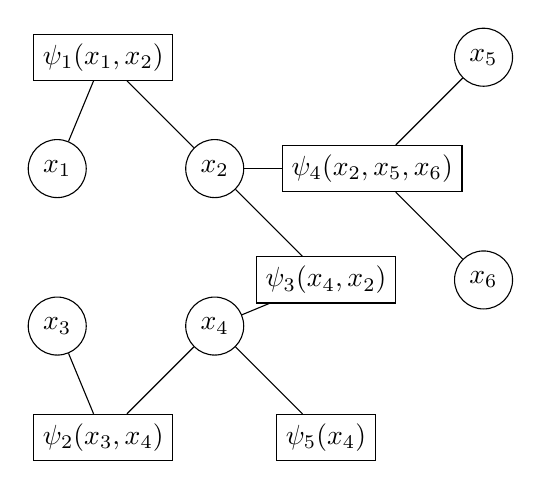
\begin{tikzpicture}[node distance=2cm]
  \node[draw, circle] (x1) {$x_1$};
  \node[draw, circle, right of=x1] (x2) {$x_2$};
  \node[draw, rectangle, right of=x2] (f4) {$\psi_4(x_2, x_5,x_6)$};
  \node[draw, circle, above right of=f4] (x5) {$x_5$};
  \node[draw, circle, below right of=f4] (x6) {$x_6$};
  \node[draw, circle, below of=x1] (x3) {$x_3$};
  \node[draw, circle, below of=x2] (x4) {$x_4$};
  \node[draw, rectangle, above left of=x2] (f1) {$\psi_1(x_1, x_2)$};
  \node[draw, rectangle, below left of=x4] (f2) {$\psi_2(x_3, x_4)$};
  \node[draw, rectangle, below right of=x4] (f5) {$\psi_5( x_4)$};
  \node[draw, rectangle, below right of=x2] (f3) {$\psi_3(x_4, x_2)$};
  \draw[-] (x1) -- (f1);
  \draw[-] (x2) -- (f1);
  \draw[-] (x3) -- (f2);
  \draw[-] (x4) -- (f2);
  \draw[-] (x4) -- (f3);
  \draw[-] (x2) -- (f3);
  \draw[-] (x2) -- (f4);
  \draw[-] (x4) -- (f5);
  \draw[-] (x5) -- (f4);
  \draw[-] (x6) -- (f4);
\end{tikzpicture}\]
where, for instance $\ux_{1\cap 3} = x_2 = \ux_{1\cap 4}$. Since the same set of variables $\ux_{a\cap b}$ can arrise from different $a$'s and $b$'s, it si more commonly written
\begin{equation}
 P(\ux) = \prod_{a} p_a(\ux_a) \prod_{i} \frac 1 {p_i(x_i)^{d_i-1}} \label{eq:BPprob}
\end{equation}
where $d_i$ is the degree of variable $i$.

\subsubsection{Bethe free energy}

Notice that any graphical model, not necessarily a tree, is subsceptible of being approximated this way. In the case of trees, it is an exact representation of the probability, while in the rest of graphs, it is an approximation. To mark the ide that it not necessarily is exact, we call the local probability distributions as beliefs and replace $p_a(\ux_a) \to b_a(\ux_a)$.

If we replace the family (\ref{eq:BPprob}) into the Gibbs free energy, we get the so called Bethe free energy is
\begin{equation}
 G_{BP}[\{b_R(\bm{s}_R)\}]  = \sum_{a} G_a[b_{a}(\ux_a)] + \sum_i (1-d_i) G_i[b_i(x_i)] \label{eq:free_en_Bethe_D}
\end{equation}
where $d_i$ is the number of factors (functions $\psi_a$) that the $i$-th variable belongs to.

The distributions $b_a(\ux_a)$ and $b_i(x_i)$ are the variables over which we minimize the free energy functional, and should approximate the marginals of the Boltzmann. For this reason, the functional minimization is not done considering the independent functions $b(\ux)$, but they are linked by the marginalization condition \index{Boltzmann distribution}
\begin{equation}
\forall_a \forall_{i\in a} \:\: b_i(x_i) = \sum_{\ux_{a \setminus i}} b_a(\ux_a). \label{eq:marginalizacion_bethe}
\end{equation}

\subsubsection*{Constrained minimization}
This relations can easily be enforced with a set of Lagrange multipliers, as we reminded you at the beginning. The Lagrange functional is
\[ L[\{b_R(\bm{s}_R), \{m_{a,i}(x_i)\}\}]  = G_{BP}[\{b_R(\bm{s}_R)\}] +  \sum_{a} \sum_{i \in a} \sum_{x_i} m_{a,i}(x_i) \left( b_i(x_i) - \sum_{\ux_{a \setminus i}} b_a(\ux_a)]  \right)\]

Extremizaiton of the Lagrange function produces the following relations
\begin{eqnarray}
 b_a(\ux_a) &=& \frac 1 z_a e^{-\beta E_a(\ux_a) }\prod_{j\in a} \prod_{b \in \partial j \setminus a} m_{b,j}(x_j) \label{eq:ba} \\
 b_i(\ux_i) &=& \frac 1 z_i e^{-\beta E_i(x_i) } \prod_{b \in \partial i} m_{b,i}(x_i) \label{eq:bi}
\end{eqnarray}
relating the local porbability distributions to the values of the local energy and the lagrange multipliers $m_{a,i}(x_i)$.

\subsubsection*{Message Passing equations}
As usual, extremization with respect to the Lagrange multipliers reproduces the constraints they are enforcing, namely eq. (\ref{eq:marginalizacion_bethe}). After writing this conditions in terms of eqs. (\ref{eq:ba,eq:bi}), we get the following relation among Lagrange multipliers:
\begin{equation}
 m_{a\to i}(x_i) = \sum_{\ux_{a \setminus i}} \frac 1 z_a e^{-\beta (E_a(\ux_a) )}\prod_{j\in a \setminus i} \prod_{b \in \partial j \setminus a} m_{b,j}(x_j)
\end{equation}

usually understood as {\bf message passing} equations.
%From now on, we will refer to a Bethe graph as a random regular graph. Like any regular graph, each node has the same connectivity $\forall_i \: d_i \equiv d$, and the random character implies that the size of the cycles grows as $\log N$. The fundamental property of a Bethe graph is that the local structure is in the form of a tree (there are no short cycles when $N\to \infty$), and this allows us to use the Bethe approximation with confidence and generally with good results \cite{cowell_bethe_exact_tree}. \index{Bethe graph}

While the approximation is exact in a tree, and is very good in a graphs with large loops, in systems with short cycles the results are usually much worse.


\subsection{A simple example: coloring trees}
Let us go back to the  {\bf Graph coloring} example. We already with this functions
\begin{eqnarray*}
\psi_{1,2,3}(x,y) &=& (1-\delta_{x,y}) \\
\psi_{4}(x,y,z) &=& (1-(1- (1-\delta_{x,y})(1-\delta_{y,z})(1-\delta_{x,z}))) \\
\psi_5(x) = 1
\end{eqnarray*}
 the probability measure
\[ P(x_1\ldots,x_6) \propto  \psi_1(x_1, x_2) \psi_2(x_3, x_4) \psi_3(x_4, x_2) \psi_4(x_2, x_5,x_6) \psi_5(x_4)\]
concentrates only on the  valid colorings.

But, this measure doesn't look as we the exponential of an energy, since the $\psi_a(\cdot)$ functions aren't equivalent to exponentials of local interactions. First, this si, in itself not a problem. Although we wrote the BP equations in the physical way, we can directly replace the energy by the functions $\psi_a$, as in \begin{equation}
 m_{a\to i}(x_i) = \sum_{\ux_{a \setminus i}} \: \psi_a(\ux_a) \: \prod_{j\in a \setminus i} \prod_{b \in \partial j \setminus a} m_{b,j}(x_j)
\end{equation}

But still, you might want not to do that. In that case, you can define
\begin{eqnarray*}
E_{1,2,3}(x,y) &=& \delta_{x,y} \\
E_{4}(x,y,z) &=& \delta_{x,y} +  \delta_{y,z} + \delta_{x,z} \\
E_5(x) = 0
\end{eqnarray*}
and use a high value of $\beta$ in your algorithm.  The energy terms now are zero for valid local configurations of colors, and 1 for invalid ones. Since $\beta$ is big, the exponentials
\[ e^{-\beta \psi_a(\cdot)} = \left\{ \begin{array}{ll}
1 & \mbox{ coloring is valid } \\
e^{-\beta} \ll 1 & \mbox{ coloring is invalid }
\end{array} \right.
\]
which for practical purposes is equivalent to the hard constraint definition.



\subsection{A clever way to count}

In particular in the tree coloring problem above, message passing equations are completely trivial, since there is no bias towards any particular color, all messages turn out to be flat
\[ m_{a\to i} (x_i) = (\frac 1 3,\frac 1 3,\frac 1 3)\]
for the case of three-colors.

Yet, there are two possible ways in which we could use the BP solution. First, we could compute the entropy
\[S = \sum_{a} S[b_a(\ux_a)]+ \sum_i (1-d_i) \sum_{x_i} S[b_i(x_i)] \qquad \mbox{where } S[b] =  -\sum_{x} b(x) \ln b(x)\]

If you evaluate in this case, you get $S=\ln 48.0$, which coincide with the 48 valid configurations, and the fact that the entropy of an uniform distribution is the log of the number of states.

You could also repeat the message passing and the entropy calculation, but forcing one node, let's say $x_4$ to have a particular color. You can do that by simply changing $\psi_5$:
\[\psi_5(x) = (1,0,0) \]
In that case, you get $S = \ln 16$, again consistent with the number of valid configurations.

\section{The zero patient problem}

{\Large \bf Note:} this is an extraction of the paper :

F. Altarelli. et. al., ``Bayesian Inference of Epidemics on Networks via Belief Propagation, '', Phys. Rev. Lett. 112, 118701 --Published 17 March 2014


\paragraph*{The SIR model on graphs \label{sec:The-SIR-model-on-graphs}}

The susceptible-infected-recovered (SIR) model of spreading is a stochastic dynamical model in discrete time defined over a graph $G=(V,E)$. At time $t$ a node $i$ can be in one of three states (\emph{infected}, \emph{suceptible} or \emph{recovered}) represented by a variable $x_{i}^{t}\in\left\{ S,I,R\right\} $.
% We assume defined known \emph{transmission probabilities} $p_{ij}\in\left[0,1\right]$ associated to each directed edge $(ij)\in E$ and a recovery probability $r_{i}\in\left[0,1\right]$ associated with each node $i$. The dynamical process is defined as follows: at each time step $t$, each node $i$ in the infected state, $x_{i}^{t}=I$ attempts contagion to susceptible neighbors in $\left\{ j\in\partial i:x_{j}^{t}=S\right\}$, each will succeed with independent probability $p_{ij}$, bringing $x_{j}^{t+1}=I$. Afterwards, node $i$ will attempt recovery with probability $r_{i}$, which if successful will bring $x_{i}^{t+1}=R$. All nodes for which none of these events succeeded conserve their prior state, i.e. $x_{k}^{t+1}=x_{k}^{t}$.
The dynamical process is defined as follows: at each time step $t$, each node $i$ in the infected state attempts to infect each one of its susceptible neighbors $\left\{ j\in\partial i:x_{j}^{t}=S\right\}$, succeeding with independent probabilities $p_{ij}\in\left]0,1\right]$ (which we assume known); then, node $i$ attempts to recover, succeeding with probability $r_{i}\in\left[0,1\right]$ (also assumed known).
The dynamics is clearly irreversible, as a given node can only undergo the transitions $S\to I\to R$, and thus a stationary condition will be reached in finite time (with all nodes either in the $S$ or $R$ state provided $r_{i}>0$).
Two important special cases of SIR are: \textbf{(a)} the Independent Cascade (IC) model, obtained when $r_{i}\equiv1$, which has been extensively studied in the related context of optimization of the spread of information \cite{kempe_maximizing_2003} and a particular sub-case of which is {\em bootstrap percolation} with threshold $\theta = 1$ (obtained when $p_{ij}\equiv 1$);
\textbf{(b)} the susceptible-infected (SI) model, obtained when $r_{i}\equiv0$. It should be noted that the IC model describes completely the SIR model for arbitrary $r_{i}$ in the infinite time limit, while the infinite time limit of the SI model is rather trivial, as all nodes in the connected component of an initially infected node will be infected at time $t\to\infty$. Nevertheless, the evolution in time can show rich and interesting characteristics.
%\begin{figure}
%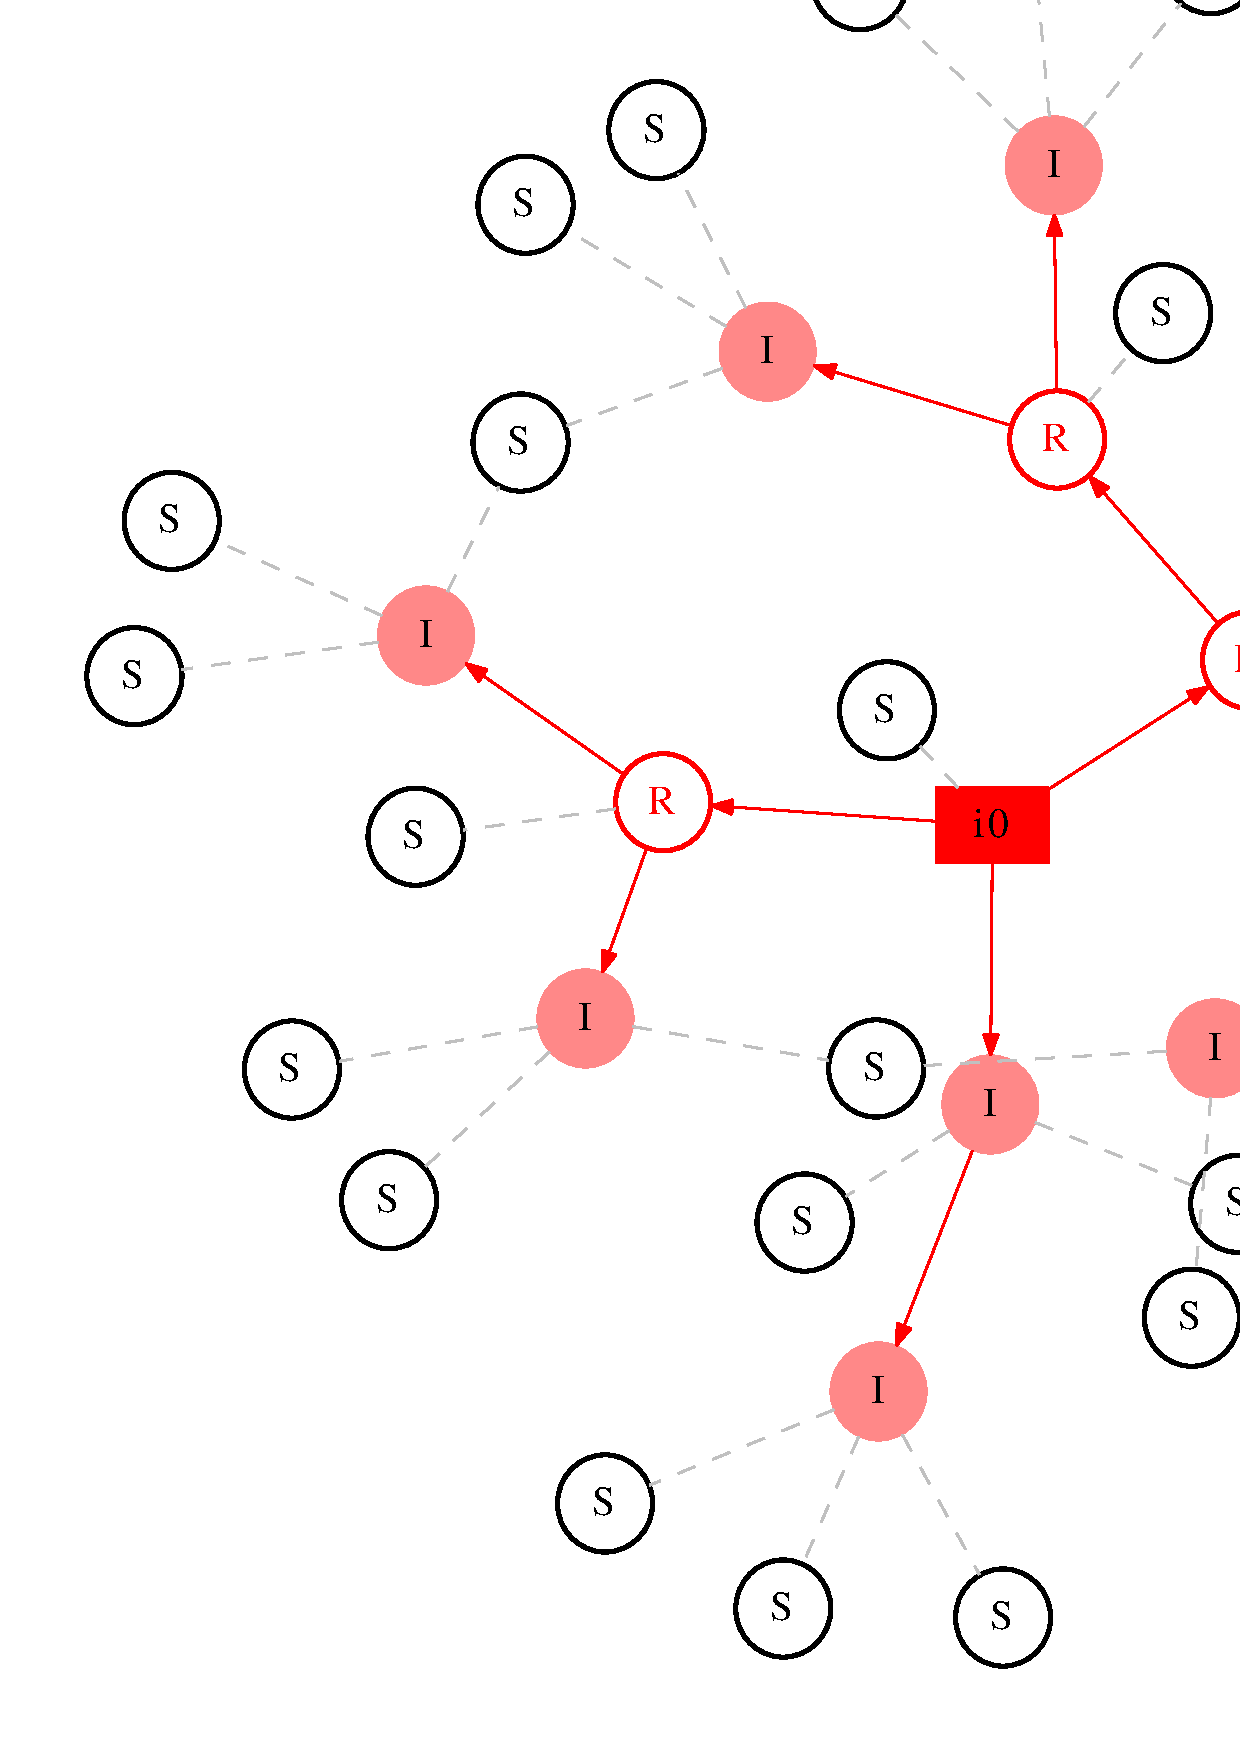
\includegraphics[width=0.65\columnwidth, angle=0]{zero_patient/epidemy}
%\caption{\label{fig:epidemy} Example of the snapshot of an epidemy after $T=3$ time
%steps. The zero patient corresponds to the square node.}
%\end{figure}


\paragraph*{Self-consistent equations for spread computation.}

Assume that a certain set of nodes starts the infection at time $t=0$,
i.e. with $x_{i}^{0}=I$. The SIR model can be re-stated as following: recovery times $g_{i}$ and {\em delay parameters} $s_{ij}$ are drawn
respectively from $\mathcal{G}_{i}\left(g_{i}\right)=r_{i}\left(1-r_{i}\right)^{g_{i}}$
and $\omega_{ij}\left(s_{ij}|g_{i}\right)=p_{ij}\left(1-p_{ij}\right)^{s_{ij}}$ for $s_{ij}\leq g_i$ and $\omega_{ij}\left(\infty|g_i\right)=\sum_{s>g_i}p_{ij}\left(1-p_{ij}\right)^{s}$;
i.e. the recovery time follows a geometric distribution and the delay
in transmission follows a geometric distribution truncated by $g_{i}$.
Afterwards, the infection times $t_{i}$ can be computed deterministically
as the ones satisfying $1=\phi_{i}=\delta\left(t_{i},\1\left[x_{i}^{0}\neq I\right]\left(\min_{j\in\partial i}\left\{ t_{j}+s_{ji}\right\} +1\right)\right)$
for every $i$. This representation makes it possible to write the
distribution of infection and recovery times $\mathbf{t},\mathbf{g}$
given the initial state $\mathcal{P}\left(\mathbf{t},\mathbf{g}|\mathbf{x}^{0}\right)=\sum_{\mathbf{s}}\mathcal{P}\left(\mathbf{s}|\mathbf{g}\right)\mathcal{P}\left(\mathbf{t}|\mathbf{x}^{0},\mathbf{g},\mathbf{s}\right)\mathcal{P\left(\mathbf{g}\right)}$
giving

\begin{eqnarray}
\mathcal{P}\left(\mathbf{t},\mathbf{g}|\mathbf{x}^{0}\right) & = & \sum_{\mathbf{s}}\prod_{i,j}\omega_{ij}\prod_{i}\phi_{i}\mathcal{G}_{i}
	\label{eq:direct}
\end{eqnarray}



\paragraph*{Bayesian inference in the SIR model}

Assume to know the sate of an epidemics at time $t=T$, i.e. the state
of every node $x_{i}^{T}\in\left\{ S,I,R\right\} $ but to possess
only probabilistic prior information about the set of initially infected
nodes; specifically, assume that nodes are initially infected with i.i.d. {\em a priori} probability $\mathcal{P}\left(\mathbf{x}^{0}\right)=\prod_{i}\gamma_{i}\left(x_{i}^{0}\right)$.
Starting with $\mathcal{P}\left(\mathbf{x}^{T}|\mathbf{t},\mathbf{g}\right)=\prod_{i}\xi_{i}\left(t_{i},g_{i},x_{i}^{T}\right)$
where $\mathcal{\xi}_{i}=\1\left[x_{i}^{T}=I,t_{i}\leq T<t_{i}+g_{i}\right]+\1\left[x_{i}^{T}=S,t_i < T\right]+\1\left[x_{i}^{T}=R,t_{i}+g_{i}\leq T\right]$,
the posterior distribution $\mathcal{P}\left(\mathbf{x}^{0}|\mathbf{x}^{T}\right)\propto\sum_{\mathbf{t,g}}\mathcal{P}\left(\mathbf{x}^{T}|\mathbf{t},\mathbf{g}\right)\mathcal{P}\left(\mathbf{t},\mathbf{g}|\mathbf{x}^{0}\right)\mathcal{P}\left(\mathbf{x}^{0}\right)$
can be expressed thanks to \eqref{eq:direct} as
\begin{equation}
\mathcal{P}\left(\mathbf{x}^{0}|\mathbf{x}^{T}\right)\propto\sum_{\mathbf{t},\mathbf{g},\mathbf{s}}\prod_{i,j}\omega_{ij}\prod_{i}\phi_{i}\mathcal{G}_{i}\gamma_{i}\xi_{i}\label{eq:Bayes}
\end{equation}



\paragraph*{Belief Propagation equations for the likelihood function}

For the derivation of the Belief Propagation (BP) equations we will rewrite \eqref{eq:Bayes} by introducing $t_{j}'=t_{j}+s_{ji}$.
Define $\phi_{ij}=\omega_{ij}\left(t'_{i}-t_{i}|g_{i}\right)\omega_{ji}\left(t'_{j}-t_{j}|g_{j}\right)$
and $\phi_{i}=\delta\left(t_{i};\1\left[x_{i}^{0}\neq I\right]\left(\min_{j\in\partial i}\left\{ t'_{j}\right\} +1\right)\right)$;
then
\[\mathcal{P}\left(\mathbf{x}^{0}|\mathbf{x}^{T}\right)\propto\sum_{\mathbf{t},\mathbf{t}',\mathbf{g}}\prod_{i<j}\phi_{ij}\prod_{i}\phi_{i}\mathcal{G}_{i}\gamma_{i}\xi_{i}.\]
In particular, one can recover a factor graph topology equivalent to the one of the original
graph of contacts (as in \cite{altarelli_optimizing_2012,*altarelli_large_2013})
by adding dynamical variables defined by triplets $(g_{i}^{(j)},t_{i}^{(j)},t'_{j})$
and regrouping terms $\psi_{i}=\phi_{i}(t_{i},\mathbf{t}'_{\partial i})\prod_{j\in\partial i}\delta(t_{i}^{(j)},t_{i})\delta(g_{i}^{(j)},g_{i})$ (See Figs.~\ref{fig:fg}c,\ref{fig:fg}d).
We obtain the effective model
\begin{equation}
\mathcal{Q}\propto\prod_{i<j}\phi_{ij}\prod_{i}\psi_{i}\mathcal{G}_{i}\gamma_{i}\xi_{i}
\label{eq:effective}
\end{equation}
in terms of which $\mathcal{P}\left(\mathbf{x}^{0}|\mathbf{x}^{T}\right)\propto\sum_{\mathbf{t},\mathbf{t}',\mathbf{g}}\mathcal{Q}\left(\mathbf{g},\mathbf{t},\mathbf{t}',\mathbf{x}^{0}\right)$.
\begin{figure}
\includegraphics[width=1.0\columnwidth]{zero_patient/fgsir}
\caption{Factor graph representations for irreversible dynamics\label{fig:fg}. (a) Original graph (b) Loopy, naive factor graph for an irreversible deterministic dynamics (c) Dual tree factor graph (d) Factor graph for the SIR model given in \eqref{eq:effective} with known epidemy age (e) Factor graph representation with unknown epidemy age.}
\end{figure}

Belief propagation equations can be written for the efficient approximate computation of marginals of \eqref{eq:effective} (See SM). The BP update of $\psi_{i}$ can be computed in time $O\left(G\cdot T\cdot\left|\partial i\right|\right)$, where $G$ is the maximum allowed recovery delay,
and the one of $\phi_{ij}$ in time $O\left(G^{2}\cdot T\right)$. In practice, $G$ can be taken constant for a geometric distribution $\mathcal G$.
A single BP iteration can be thus computed in time $O\left(T\cdot G^{2}\cdot\left|E\right|\right)$. We remark that the BP equations for the posterior distribution are exact (and have a unique solution) on tree factor graphs \cite{pearl_reverend_1982}. As the topology of the factor graph mirrors the one of the original graph, \eqref{eq:effective} allows the exact computation of posterior marginals for the SIR model on tree graphs (at difference with the DMP method).

\paragraph*{Unknown epidemy age}
The start time of the epidemy was assumed up to now to be known, but this may be unrealistic. Coping with the case of unknown initial time is easy; starting with an upper bound on the epidemic duration, it suffices to consider the dynamical process to start from the all-susceptible state but to allow nodes to be spontaneously infected at an arbitrary time with (small) uniform probability. This is equivalent to the addition of a fictitious virtual neighbor to every node with no constraint in its activation time besides the prior probability $\varepsilon_i(g''_i,t''_i,t_i)=\delta(t''_i,\infty)(1-2\gamma)+\gamma$ of spontaneous infection (See Fig.~\ref{fig:fg}e).%The case of known epidemy age, with a single epidemic origin, is recovered by considering the self-infection probability to be zero for times different from the initial one.

\paragraph*{Identification of a single source}
Through out the rest of the paper we restrict ourselves to random regular graphs of degree $k=4$ and $N=1000$ nodes with homogeneous propagation probability $p_{ij}\equiv p$ and recovery probability $r_i\equiv r$ in order to make comparison with other inference methods simpler. An example of inference for an epidemy with recovery and transmission probabilities $\lambda=\mu=0.5$ is depicted in Fig.~\ref{fig:infertimes}. For each node, an infection time distribution is computed as a BP marginal and the mean and standard deviation of this ditribution are plotted against the true time.
We compared the inference performance of BP with the one of DMP in the case of a single epidemic source. The DMP method iterates the forward probabilistic transmission equations of \cite{karrer_message_2010} to obtain single-site trajectory probability distributions. Afterwards, using a single-site factorization hypothesis for joint distribution at the observation time, it gives a simple factorized expression of the likelihood of the observed epidemy. DMP is shown \cite{lokhov_inferring_2013} to outperform other more classical estimations of the epidemy origin \cite{shah_detecting_2010,*shah_rumors_2011,comin_identifying_2011}.
%In figure \ref{fig:rank_vs_lambda_T6_mu1} and \ref{fig:rank_vs_lambda_T11_mu05} we show the average normalized ranking of BP, DMP and Jordan centrality \cite{shah_detecting_2010,shah_rumors_2011,comin_identifying_2011} estimations. For small observations times ($T=5$ in figure \ref{fig:rank_vs_lambda_T6_mu1}) BP is slightly more accurate than DMP. Note that for short times the epidemy structure is particularly simple on expander graphs. For bigger epidemies BP substantially outperforms DMP in terms of accuracy, in some cases outstandingly (see Fig.~\ref{fig:rank_vs_lambda_T11_mu05}).
\begin{figure}
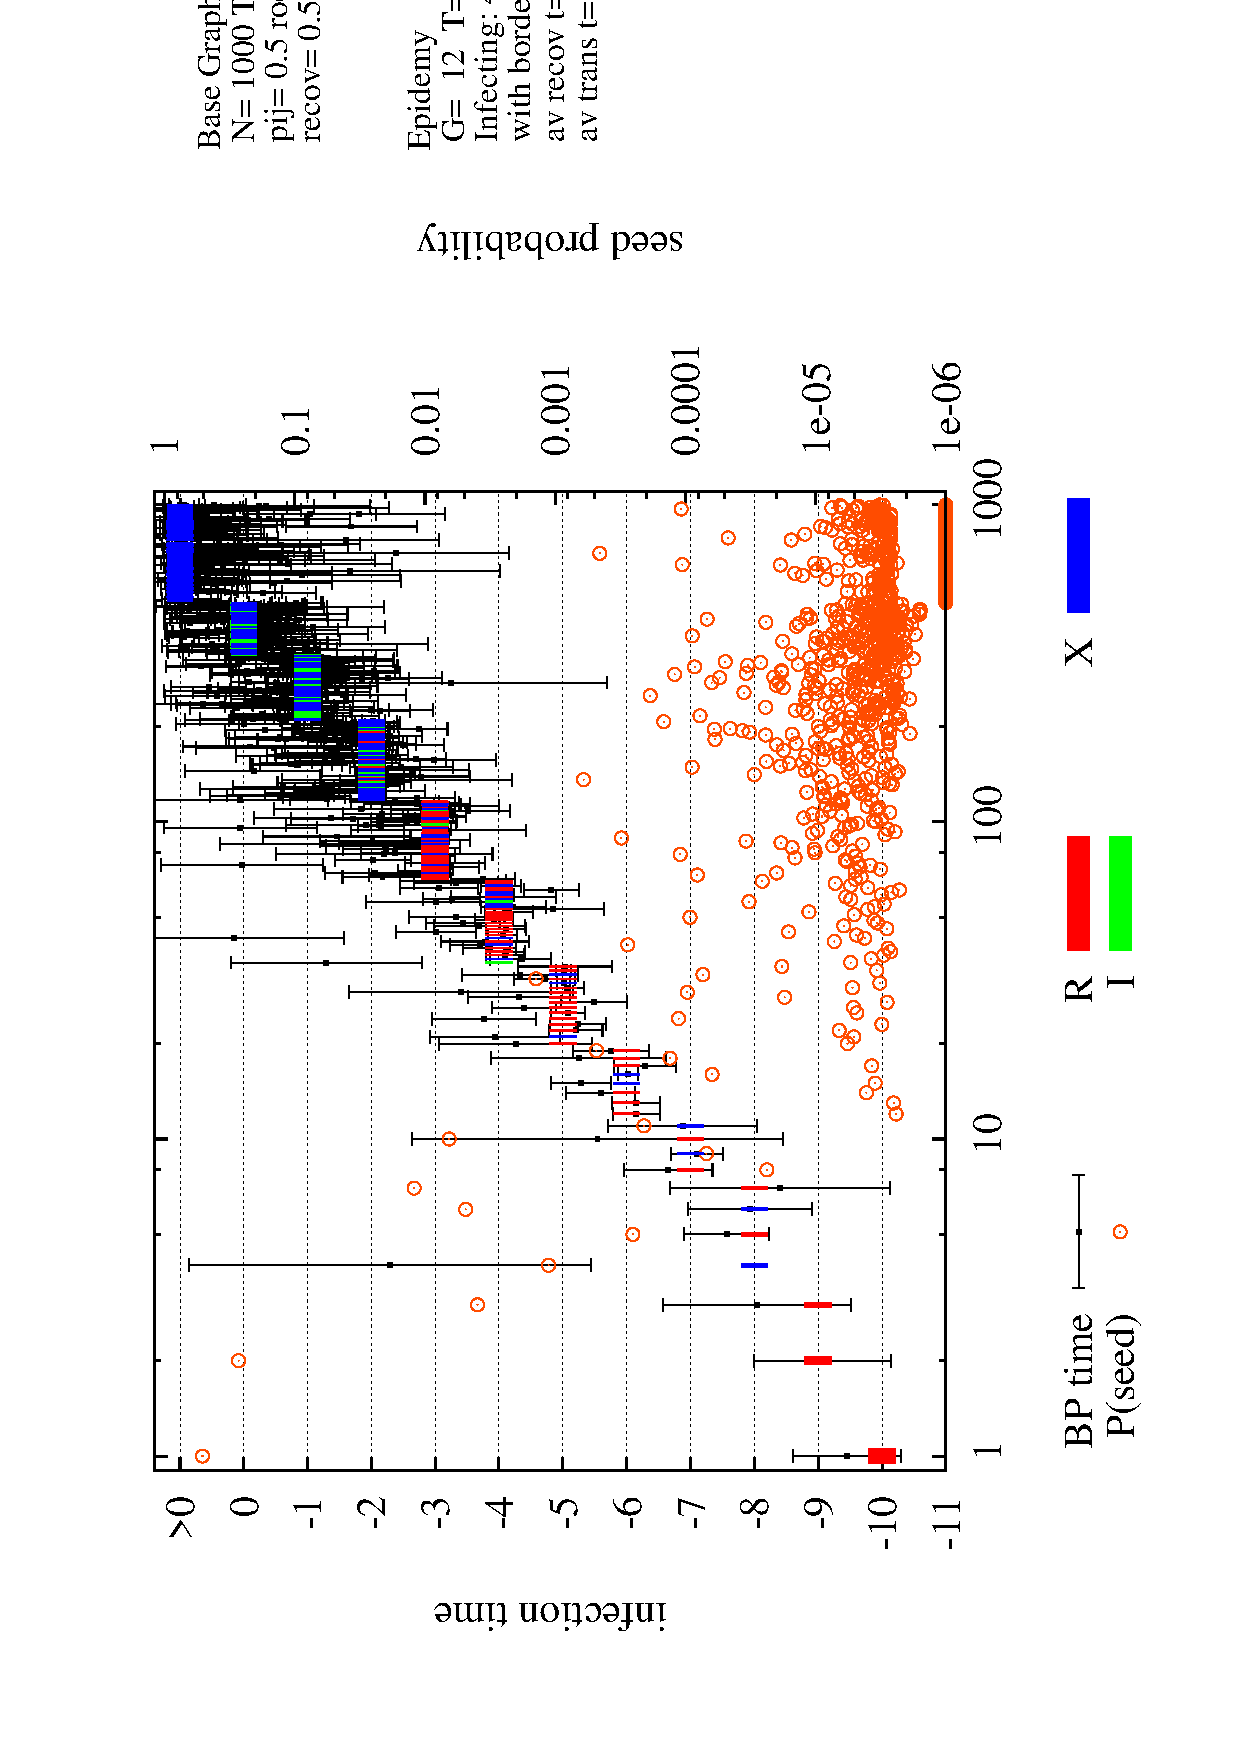
\includegraphics[height=1.0\columnwidth, angle=270]{zero_patient/infertimes}
\caption{(Color online) An example of inference on a RRG with $N=1000,k=4$, with $\lambda=\mu=0.5$ and prior seed probability $10^{-6}$, and observations at time $T=0$ on $\xi=0.7$ of the nodes on an epidemy with $t_0=-10$. Each point in the x axis corresponds to a vertex on the graph. Nodes are ordered by their real infection time (blocks, R=recovered, I=infected and X=unknown). The mean and standard deviation of their BP posterior marginal distribution of infection time is plotted (black dots and error bars) along with the marginal posterior probability of self-infection (orange, circles, right axis).\label{fig:infertimes} }
\end{figure}

Two methods are used as benchmarks: Jordan centrality \cite{shah_detecting_2010,shah_rumors_2011,comin_identifying_2011} and DMP. In figure \ref{fig:rank_vs_lambda_T11_mu05} we show the average normalized rank given to the true zero patient by BP, DMP and Jordan centrality over $10^3$ instances with observation time $T=10$ and recovery probability $\mu=0.5$. Since DMP requires a defined value of the observation time, we here assume that $T=10$ is known for both DMP and BP. It is seen how BP outperforms DMP by a large margin in the probability of finding the epidemy origin. The inset shows also a remarkable difference in the normalized ranking of the true origin given by all three algorithms, again BP outperforming the other two.
%For small observations times ($T=5$ in figure  \ref{fig:rank_vs_lambda_T6_mu1}) BP is slightly more accurate than DMP. Note that short times the epidemy structure is particularly simple on expander graphs. For bigger epidemies BP substantially outperforms DMP in terms of accuracy, in some cases outstandingly (see Fig. \ref{fig:rank_vs_lambda_T11_mu05}).


%DA RIVEDERE IN BASE AI RISULTATI: As in any belief propagation approach, we rely upon convergence to get an estimate of the desired quantities. When epidemy sizes grow (see purple dotted line) the message passing heuristic begin failing to converge within 300 iteration steps. After examining not convergent samples we decided to use the information from BP even when convergence is not reached. It can be seen in Fig. \ref{fig:rank_vs_lambda_T11_mu05} that in this regime the predictions obtained are worse than those obtained with DMP, but still better than Jordan centrality, and better than a random estimation.

%\begin{figure}
%\includegraphics[width=0.65\columnwidth, angle=270]{zero_patient/T6_rank_vs_lambda_mu1.eps}
%\caption{\label{fig:rank_vs_lambda_T6_mu1} }
%\end{figure}


\begin{figure}
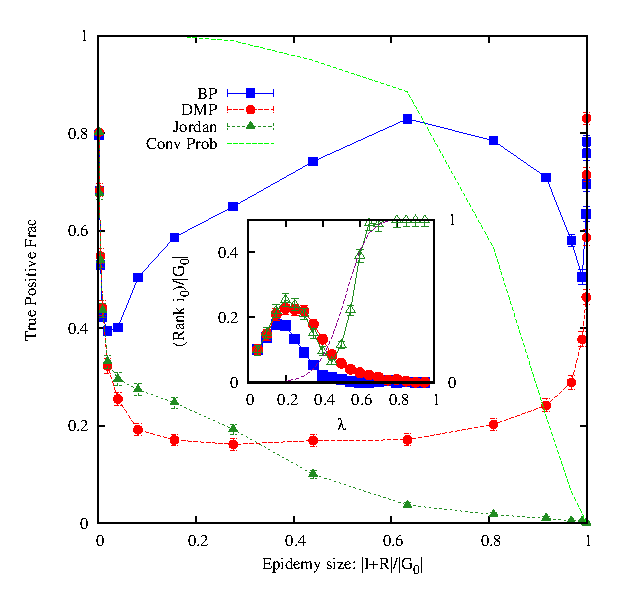
\includegraphics[width=1\columnwidth, angle=0]{zero_patient/T11_rank_vs_lambda_mu05}
\caption{\label{fig:rank_vs_lambda_T11_mu05} Normalized rank given to the true zero patient by Jordan, DMP and BP methods, as a function of the transmission probability $\lambda$, averaged over $10^3$ instances of $N=1000, k=4$ RRG with observation time $T=10$. Most relevant part is $0.2<\lambda<0.8$ where the epidemy size (purple, right axis) spans most of its range. For too large epidemies BP has convergence problems (green, right axis), nevertheless some relevant information is still present in the (unconverged) marginals. The inner plot shows the probability of finding the true origin of the epidemy using DMP and BP as a function of the average epidemy size for each value of $\lambda$.}
\end{figure}



\paragraph*{Incomplete information}

In a more realistic setup, the state of many nodes in the population is usually not known. Calling $\xi$ the fraction of unobserved sites (denoted in state $X$), we test the average ranking given to the real zero patient by BP, and compared it with other three methods in Fig.~\ref{fig:rank_vs_obs}. We found that DMP can be improved over its original presentation if the dyamics MP equations are not iterated over all the nodes of the graph, but only over the connected component of $I,R$ and $X$ nodes. We refer to this version as DMP-restricted or DMPr (see SM for details). Jordan centrality is also computed over this connected component as in \cite{lokhov_inferring_2013}. BP is quite efficient in this regime, finding the true zero patient in more than $75\%$ of instances up to $60\%$ of unobserved sites (inner plot), and outperforming all other methods for almost all $\xi$.% and \ref{fig:perfect_inf}.

\begin{figure}
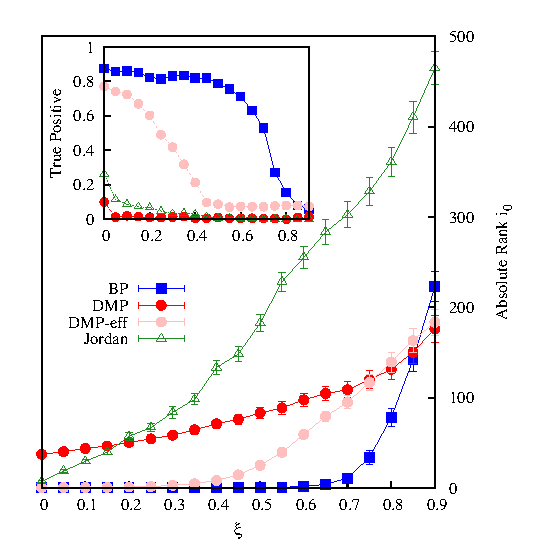
\includegraphics[width=1\columnwidth, angle=0]{zero_patient/T11_rank_vs_obs}
\caption{\label{fig:rank_vs_obs} }
\end{figure}

\begin{figure}
\includegraphics[width=1\columnwidth, angle=0]{zero_patient/multiseeds}
\caption{Inference of multiple seeds with $r=1,p_{ij}=0.5$, seed probability $0.002$ and variable $T-t_0$ (unknown to the inference algorithm). Inference was attempted for each of 1 000 instances for every $T-t_0$, and the the sum of the rankings of the true seeds in the outcome order is plotted vs. the true number of seeds. Inset: the average area of the ROC curve. Each ROC curve was computed restricted to the epidemic subgraph.\label{fig:multiseeds} }
\end{figure}
\paragraph*{Inference of multiple sources}
If the origin of the epidemics is not a single source, but a set of sources, methods based on the exhaustive exploration of initial states like DMP suffer a combinatorial explosion. This problem does not affect BP, as the trace over initial conditions is performed directly within the framework. We show in Fig.~\ref{fig:multiseeds} experiments with multiple seeds, showing that effective inference can also be achieved in this regime.

\paragraph*{Dynamically evolving networks}
We studied the case of dynamically evolving networks, in which the transmission probility $p_{ij}$ depends on time (representing the time-evolution of interactions between agents). For this purpose, we employed the interesting dataset \cite{isella_whats_2011}, corresponding to a large list of time-stamped face-to-face contacts between couples of visitors in a cultural event. We aggregate the 20 second resolution of the data into $T$ effective time steps, and simulate the progression of a virtual epidemy initiated by a random visitor. We employed the following set of parameters: probability $p^{20s}_{ij}=0.1$ of contagion in a 20 second interval, recovery probability $r=0.1$, and $T-t_0=30$. We employed the last four days of the event, in which the volume of visitors was larger, and simulated 2000 random propagations. We kept the 50 epidemies with larger number of infected individuals ($98\pm 14$). The correct origin was identified perfectly in 13 cases (26\%), and in general its normalized ranking was in average $0.07\pm0.11$. Finally, also infection times were recovered with good accuracy: the probability assigned to the correct infection time (for infected individuals) was in average $0.53\pm 0.06$, and the average absolute error in the infered infection time was $0.76\pm 0.23$.

%\paragraph*{Conclusions}

%A more general formulation that includes recovery probabilities $r_{i}$ that depend on the time after infection $s=t-t_{i}$ and/or the absolute time $t_{i}$, and can also be incorporated in the BP formalism in a straightforward way.
%We have shown how to use the Bethe approximation and the corresponding cavity equations in the context of zero patient inference in epidemics. The construction of a local tree-like graph is nontrivial, resulting in a set of BP equations for the SIR model that, when converged, approximate the marginals distributions of infection times for each node. Improvement over previous methods can be grouped in three aspects:
%\begin{enumerate}
%\item Formality of the approach and controllability of the approximation
%\item Accuracy of the predictions
%\item Generality, scalability and flexibility of the method.
%\end{enumerate}

%At variance with the uncontrolled factorization of probabilities done for the Dynamic Message Passing method, our approach is based on the Bethe approximation which is exact when the underlaying graph is a tree. Not surprisingly the results obtained this way outperforms the Jordan Centrality, the DMP and the improved version of DMP we presented in this paper, giving both better average ranking for the true zero patient, and higher true positive ratio.

%Bethe approximation seems to be the natural approach to zero patient inference since it sets a very general frame form which other tasks are attained in a straightforward manner. For instance, inferring two or more zero patients is not accessible with Jordan Centrality (at least in its standard way), and renders the computation time combinatorial in the number of seeds for DMP, while in BP it entails no particular upheaval. The  observation time also comes natural in the BP approach, while DMP requires an \textit{adhoc} method for it. Partial information, like unobserved nodes, or over information, like knowing the precise infection time of some nodes, can be directly included in the BP formalism. Finally, dynamics networks are also just a step away of our presentation, allowing a description of a more realistic situation.

\begin{subappendices}

\section{Functionals and Lagrange Multipliers}


\subsubsection*{Functionals}

A functional is a function that takes a function as its input and produces a scalar value as its output. More formally, let $X$ be a set of functions, and let $F$ be a function that maps $\mathcal C$ to the set of real numbers $\mathbb{R}$. Then, we say that $F$ is a functional, and we write:
$$F:\mathcal{C} \rightarrow\mathbb{R}$$
In this context, the elements of $\mathcal C$ are often called the "arguments" or "inputs" of the functional $F$.

Sure, I'd be happy to explain how derivatives with respect to functional arguments are done.

When we take the derivative of a functional with respect to one of its arguments, we're asking how much the value of the functional changes as we change the function at that argument.

Formally, let $F:\mathcal{C} \rightarrow \mathbb{R}$ be a functional that maps a set of functions $\mathcal{C}$ to the real numbers, and let $f \in \mathcal{C}$ be a function in the domain of $F$. Then, the derivative of $F$ with respect to $f$ is still a functional denoted by $D\:F[f]$ or $\frac{\delta F}{\delta f}[f,h]$, and is defined as follows:
$$D\:F[f, h] = \lim_{\epsilon\rightarrow 0} \frac{F[f+\epsilon h] - F[f]}{\epsilon}$$
where $h$ is a small perturbation to $f$. In other words, we're looking at how much the value of $F$ changes as we perturb $f$ in the direction of $h(x)$, and then divide by the size of the perturbation $\epsilon$.

Note that the derivative of a functional with respect to one of its arguments is itself a functional. The perturbation $h(x)$ is taken as a unit norm function. If we take $h(x) = \delta(x-x_0)$, the derivative is a function of $x_0$, and a functional of $f(x)$. In such case, the derivation is carried as if $f(x)$ was itself a number. Lets see an example:

One of the simplest functionals, is the intgral of a function, since it produces a real value:
\[ I[f] = \int_a^b f(x) \ud x\]
where $f(x)$ is a function defined on the interval $[a,b]$.

The derivative of $I[f]$ with respect to $f$ is given by:
$$\frac{\delta I[f]}{\delta f(x')} = \lim_{\epsilon\rightarrow 0} \frac{I[f+\epsilon \delta(x-x')] - I[f]}{\epsilon} = \lim_{\epsilon\rightarrow 0} \frac{1}{\epsilon}\int_a^b \delta(x-x')\epsilon dx = \delta(x-x')$$
where $\delta(x-x')$ is the Dirac delta function. This result tells us that the derivative of $I[f]$ with respect to $f$ at the point $x'$ is equal to the Dirac delta function evaluated at $x'$.


%In particular, if $F$ is a linear functional, then $DF(f)$ is also a linear functional.


Consider the functional $L[f]$ defined by:
$$L[f] = \int_a^b \sqrt{1+(f'(x))^2}dx$$
where $f$ is a function defined on the interval $[a,b]$. This functional takes a function $f$ as its argument, and returns the length of the curve defined by the graph of $f$ over the interval $[a,b]$.

To find the derivative of $L[f]$ with respect to $f$, we can use the calculus of variations. Specifically, we seek a function $h$ that minimizes the value of the functional:
$$J[h] = L[f+\epsilon h]$$
subject to the constraint that $h(a) = h(b) = 0$. Intuitively, we're looking for the function $h$ that produces the smallest change in the length of the curve as we perturb $f$ by a small amount $h$.
%
% Using the Euler-Lagrange equation, we can find the function $h$ that minimizes $J[h]$ and hence the derivative of $L[f]$ with respect to $f$. The Euler-Lagrange equation for $J[h]$ is given by:
%
% \[ \frac{d}{dx}\left(\frac{\partial}{\partial f'}\sqrt{1+(f'(x)+\epsilon h'(x))^2}\right) - \frac{\partial}{\partial f}\sqrt{1+(f'(x)+\epsilon h'(x))^2} = 0\]
% Expanding the square root and using a Taylor series expansion, we can simplify this equation to:
% \[\frac{d}{dx}\left(\frac{f'(x)+\epsilon h'(x)}{\sqrt{1+(f'(x))^2}}\right) - \frac{f''(x)\epsilon h'(x)}{\sqrt{1+(f'(x))^2}} = 0\]
%
% Dividing through by $\epsilon$ and taking the limit as $\epsilon \rightarrow 0$, we obtain:
% \[\frac{d}{dx}\left(\frac{f'(x)}{\sqrt{1+(f'(x))^2}}\right) - \frac{f''(x)}{\sqrt{1+(f'(x))^2}} = 0\]
% This is a second-order differential equation that can be solved to find the function $h$ that minimizes $J[h]$. Substituting this function into the expression for $J[h]$ and taking the derivative with respect to $\epsilon$ at $\epsilon = 0$, we obtain the derivative of $L[f]$ with respect to $f$:
%
% \[\frac{\delta L[f]}{\delta f(x')} = \frac{f''(x')}{\sqrt{1+(f'(x'))^2}}\]
% This tells us how much the length of the curve changes as we perturb $f$ by a small amount at the point $x'$.

Derivatives with respect to functional arguments are an important tool in many areas of mathematics, including calculus of variations, optimization, and partial differential equations.

\subsubsection*{Lagrange Multipliers}
The method of Lagrange multipliers is a technique used in optimization to find the maximum or minimum of a function subject to one or more constraints.
Suppose we want to find the maximum or minimum of a function $f(x_1, x_2, ..., x_n)$ subject to a set of constraints of the form:
\begin{equation}
    g_i(x_1, x_2, ..., x_n) = 0, \quad i = 1, 2, ..., m,
\end{equation}
where $m$ is the number of constraints. To solve this problem using the method of Lagrange multipliers, we introduce a set of Lagrange multipliers $\lambda_1, \lambda_2, ..., \lambda_m$, and construct the Lagrangian function:
\begin{equation}
    L(x_1, x_2, ..., x_n, \lambda_1, \lambda_2, ..., \lambda_m) = f(x_1, x_2, ..., x_n) - \sum_{i=1}^m \lambda_i g_i(x_1, x_2, ..., x_n).
\end{equation}
We then find the critical points of the Lagrangian function by setting its partial derivatives with respect to each variable to zero:
\begin{equation}
    \frac{\partial L}{\partial x_i} = 0, \quad i = 1, 2, ..., n,
\end{equation}
\begin{equation}
    \frac{\partial L}{\partial \lambda_i} = 0, \quad i = 1, 2, ..., m.
\end{equation}
The solutions to these equations give us the values of $x_1, x_2, ..., x_n$ and $\lambda_1, \lambda_2, ..., \lambda_m$ that satisfy both the constraints and the maximum or minimum conditions.

The Lagrange multipliers have the interpretation of being the rate of change of the function $f$ with respect to the constraints $g_i$. That is, if we move along the constraint surface in the direction of the $i$th constraint, then the rate of change of the function $f$ is given by the Lagrange multiplier $\lambda_i$.

%In summary, the method of Lagrange multipliers is a powerful technique for solving optimization problems with constraints. It involves introducing Lagrange multipliers and constructing a Lagrangian function, which is then optimized by finding the critical points of the function. The Lagrange multipliers have a physical interpretation as the rate of change of the function with respect to the constraints, and can be used to gain insight into the behavior of the system being optimized.
\end{subappendices}



\chapter{Cascade epidemics and contact tracing}

\section{Effects of contact tracing and quarantine}

\end{document}
